\documentclass{book}
%% Fix so sections are manually numbered
\setcounter{secnumdepth}{0}
%% Stop text from indenting
\setlength\parindent{0pt}

%% Graphics are stored in the graphics path
\usepackage{graphicx}
\graphicspath{ {./Latex} }

%% Making hyperlinks in the table of contents
\usepackage{hyperref}
\hypersetup{
    colorlinks,
    citecolor=black,
    filecolor=black,
    linkcolor=blue,
    urlcolor=black
}

\title{Jammertest Testplan}
\author{Jammertest Consortium}
\date{ }

\begin{document}
\maketitle

\includegraphics[scale=0.1]{graphics/NPRA.png}

\tableofcontents

\section{Introduction}
Jammertest is a government initiative to create a tasted for industry, academia and other authorities in ensure robust use of Global Navigation Satellite Systems (GNSS). A testbed is a controlled environment where activities that are not allowed under normal conditions can be carried out safely under control of the authorities. Jammertest is a specific type of testbed where five Norwegian authorities have come together and creates an environment where GNSS jamming, spoofing and meaconing is present under controlled conditions in a real world outdoor environment.

This test plan describes all planned test cases that can be executed at the Jammertest event at Bleik, Andøya.For Jammertest a selected number of tests from this plan will be included in a transmission plan. The transmission plan is available just before the Jammertest event starts. After the Jammertest event the organizers will publish a transmission log that contains all tests that where run and at what time they were run. The time schedule during the live event will be given in local time, UTC time + 2 (CEST).

A machine readable test plan is available in JSON format, and this document is built based on the machine readable test plan. The numbering of the tests are presistant and will, hence over the years the same number will indicate the same test and new varieties of the tests will be given new numbers.

Tests are stacked together in large test groups and test and varieties of tests are linked to the test group and tests via a numbering system.

TestGroup.Test.TestVariety

Some tests have 2 numbers, test group and the specific test. Others may have 3 numbers due to the fact that a specific variety has been added. For example is power is reduced a new test variety is created.


Naming of the jammers are linked to the jammers specification document that list all jammers with relevant information about the jammer.

This document is auto updated based on changes to the machine readable file, there is no version code apart from the time and date when the document is produced. In the Github repository all produced versions are stored in the history of this file.

\section{Spesifications of tests}
Tests are split into large test groups. Within a testgroup there is a logical connection between the tests that related to the usecase. Hence each test group has a \textit{Rationale} why this is test is created, this also gives a hint about what to expect when subjected to this test. As we are on the bleeding edge of GNSS disturbances this section may be updated between Jammertests based on new knowledge created. 

Technical details are stored in the \textit{Test setup} section of the document. The \textit{Areas} section of the document refer to where the test can be run. Here participants need to keep track of in which area they where and this also gives and indication of which areas where the organizers are capable of running the tests. There is also a location out at sea.

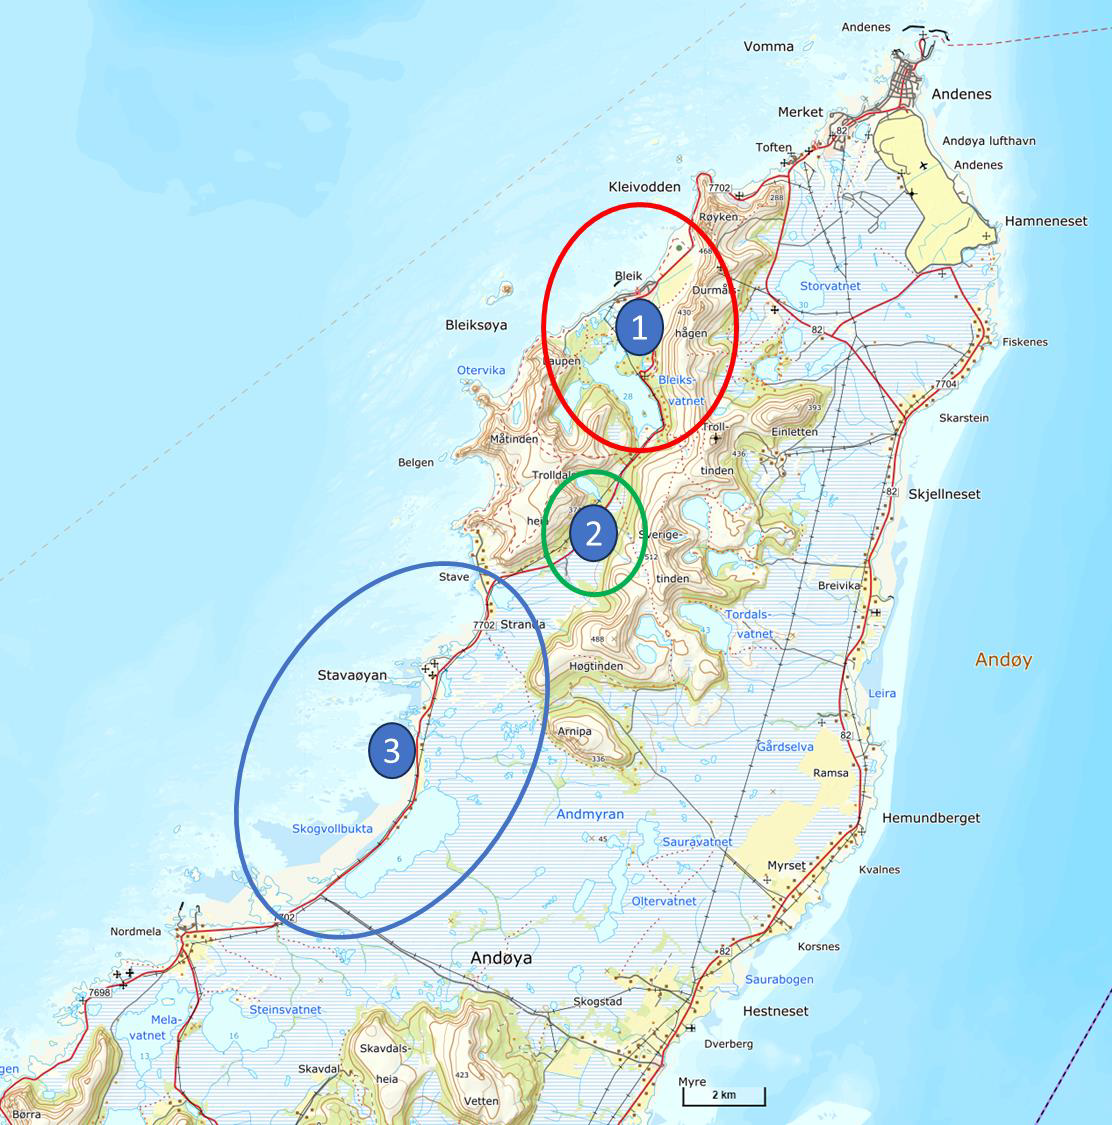
\includegraphics[scale=0.4]{graphics/locations.png}

For those wanting more information or have feedback about the test group a technical contact is provided. 

For each test group a set of tests and test varieties are listed with their unique identification number and and name, a text that describes the test. An approximate power number for the transmission. If the test is an automated ramp test then the power range is given. A time estimate of how long the test takes to conclude is given in minutes. Between tests there are also grace periods to allow systems to regain normal operation. These are not given as they are dependent on equipment and needs to be discussed with participants beforehand. The actual grace time will be calculated from the transmission log. The location of the transmitter equipment is also given in the test, this is a coarse human readable description of where the transmitting antenna is located. All participants are encouraged to make their own notes on the location of the transmitting antenna if detailed information is needed. There is also a comment field that can be used to document any other relevant information related to the specific test. 

\chapter{Description of tests}
% Content below is autogenerated 
\chapter{0 Supplemental periods}

\section{0.0: Mandatory briefings}

\subsection*{Rationale}

In order for everyone to have a good time and ensure a safe event, there will be mandatory briefings.

\subsection*{Test description}

These are the mandatory safety briefings. These briefings will also be used to go through the plan for the day and the afternoon brief will contain important observations from the day and a safety debrief.

\subsection*{Additional information}

Mandatory!

\section*{Tests within this test group}

\subsection{0.0.1  Mandatory morning briefing}

\textcolor{lightgray}{\noindent\rule[0.5ex]{\linewidth}{1pt} }
No RF interference expected.
\subsubsection*{Power or power range}
'N/A'\subsubsection*{Test bands/constellation}
'N/A'
\subsubsection*{Transmitter equipment}
'N/A'
\\\subsection{0.0.2  Mandatory afternoon (de)briefing}

\textcolor{lightgray}{\noindent\rule[0.5ex]{\linewidth}{1pt} }
No RF interference expected.
\subsubsection*{Power or power range}
'N/A'\subsubsection*{Test bands/constellation}
'N/A'
\subsubsection*{Transmitter equipment}
'N/A'
\\\section{0.1: Grace period}

\subsection*{Rationale}

In order for equipment to return to normal operation after interference, a grace period is provided between tests.

\subsection*{Test description}

This period can be used to make sure that equipment is ready for upcoming tests.

\section*{Tests within this test group}

\subsection{0.1.1  Grace period}

\textcolor{lightgray}{\noindent\rule[0.5ex]{\linewidth}{1pt} }
No RF interference expected in this test.
\subsubsection*{Power or power range}
'N/A'\subsubsection*{Test bands/constellation}
'N/A'
\subsubsection*{Transmitter equipment}
'N/A'
\\\section{0.2: Booking slots}

\subsection*{Rationale}

Some participants require more specialized ad-hoc tests. Tests in this test group will allow participants to book a time slot and equipment to perform their own tests.

\subsection*{Test description}

Tests in this group are available for booking.

\section*{Tests within this test group}

\subsection{0.2.1  Jamming booking slot}

\textcolor{lightgray}{\noindent\rule[0.5ex]{\linewidth}{1pt} }
This test require prebooking.
\subsubsection*{Power or power range}
'N/A'\subsubsection*{Test bands/constellation}
'N/A'
\subsubsection*{Transmitter equipment}
'N/A'
\\\section{0.3: Ad hoc tests}

\subsection*{Rationale}

Some tests can not be planned for in advance. These tests may include new scenarios or altered tests based on observations during the event.

\subsection*{Test description}

Tests in this group are created ad hoc during the event. Test comments will describe the setup.

\section*{Tests within this test group}

\subsection{0.3.1  Ad hoc test}

\textcolor{lightgray}{\noindent\rule[0.5ex]{\linewidth}{1pt} }
See log comment for description.
\subsubsection*{Power or power range}
'N/A'\subsubsection*{Test bands/constellation}
'N/A'
\subsubsection*{Transmitter equipment}
'N/A'
\\\chapter{1 Jamming}

\section{1.1: Continuous stationary low power jamming with commercially available jammers}

\subsection*{Rationale}

The main objective is to observe how the J/S signal affect the availability of PNT, and/or how it produces inaccurate PNT data, when the jamming signal (J) is generated by low-power jammers commercially available online. Additionally, as these types of jammers are the ones one is most likely to meet in the real world, capturing and storing the signals from these jammers for later use in labs could be useful.

\subsection*{Test description}

All tests will be performed with the jammers place 1 to 1.5 meters above ground (like on top of a vehicle) or on a stand. Unless otherwise stated, jammers will be in ``maximum'' posistion, meaning all relevant antennas are switched on and power is set to as high as possible. Runtime and pauses between tests is set in the transmission plan document.

\subsection*{Additional information}

Specification of jammers can be found in Appendix G. Jammer power levels are based on 2023/2024 measurements. ``Test bands/constellation'' refers to potentially afflicted signal types of the 4 GNSS constellations GPS, GLONASS, Galileo, and BeiDou, from the jammer in question. This information must be considered indicative only. The main principle for putting a signal type in the ``Test bands/constellation'' list for a given jammer or test, is that measurements done by NKOM indicate that the output signal of the jammer covers the center frequency of the given GNSS band(s).

\section*{Tests within this test group}

\subsection{1.1.1  Jammer S1.1}

\textcolor{lightgray}{\noindent\rule[0.5ex]{\linewidth}{1pt} }
Test with jammer S1.1
\subsubsection*{Power or power range}
Min: 0.01 W\\Max: 0.0316 W\subsubsection*{Test bands/constellation}
'L1', 'E1', 'B1C', 'B1I'
\subsubsection*{Transmitter equipment}
'S1.1'
\\\subsection{1.1.2  Jammer S1.2}

\textcolor{lightgray}{\noindent\rule[0.5ex]{\linewidth}{1pt} }
Test with jammer S1.2
\subsubsection*{Power or power range}
Min: 0.01 W\\Max: 0.0316 W\subsubsection*{Test bands/constellation}
'G1', 'L1', 'E1', 'B1C', 'B1I'
\subsubsection*{Transmitter equipment}
'S1.2'
\\\subsection{1.1.3  Jammer S1.3}

\textcolor{lightgray}{\noindent\rule[0.5ex]{\linewidth}{1pt} }
Test with jammer S1.3
\subsubsection*{Power or power range}
Min: 0.01 W\\Max: 0.0316 W\subsubsection*{Test bands/constellation}
'L1', 'E1', 'B1C', 'B1I'
\subsubsection*{Transmitter equipment}
'S1.3'
\\\subsection{1.1.4  Jammer S2.1}

\textcolor{lightgray}{\noindent\rule[0.5ex]{\linewidth}{1pt} }
Test with jammer S2.1
\subsubsection*{Power or power range}
Min: 0.0316 W\\Max: 0.1 W\subsubsection*{Test bands/constellation}
'G1', 'L1', 'E1', 'B1C', 'B1I', 'G2', 'L2', 'E5b', 'B2b', 'B2I', 'G3', 'L5', 'E5a', 'B2a'
\subsubsection*{Transmitter equipment}
'S2.1'
\\\subsection{1.1.5  Jammer S2.2}

\textcolor{lightgray}{\noindent\rule[0.5ex]{\linewidth}{1pt} }
Test with jammer S2.2
\subsubsection*{Power or power range}
Min: 0.0316 W\\Max: 0.1 W\subsubsection*{Test bands/constellation}
'G1', 'L1', 'E1', 'B1C', 'B1I', 'G2', 'L2', 'E5b', 'B2b', 'B2I', 'G3', 'L5', 'E5a', 'B2a'
\subsubsection*{Transmitter equipment}
'S2.2'
\\\subsection{1.1.6  Jammer S2.3}

\textcolor{lightgray}{\noindent\rule[0.5ex]{\linewidth}{1pt} }
Test with jammer S2.3
\subsubsection*{Power or power range}
Min: 0.0316 W\\Max: 0.1 W\subsubsection*{Test bands/constellation}
'G1', 'L1', 'E1', 'B1C', 'B1I', 'G2', 'L2', 'E5b', 'B2b', 'B2I', 'G3', 'L5', 'E5a', 'B2a'
\subsubsection*{Transmitter equipment}
'S2.3'
\\\subsection{1.1.7  Jammer S2.4}

\textcolor{lightgray}{\noindent\rule[0.5ex]{\linewidth}{1pt} }
Test with jammer S2.4
\subsubsection*{Power or power range}
Min: 0.0316 W\\Max: 0.1 W\subsubsection*{Test bands/constellation}
'G1', 'L1', 'E1', 'B1C', 'B1I', 'G2', 'L2', 'E5b', 'B2b', 'B2I', 'G3', 'L5', 'E5a', 'B2a'
\subsubsection*{Transmitter equipment}
'S2.4'
\\\subsection{1.1.8  Jammer U1.1}

\textcolor{lightgray}{\noindent\rule[0.5ex]{\linewidth}{1pt} }
Test with jammer U1.1
\subsubsection*{Power or power range}
'N/A'\subsubsection*{Test bands/constellation}
'G1', 'L1', 'E1', 'B1C', 'B1I'
\subsubsection*{Transmitter equipment}
'U1.1'
\\\subsection{1.1.9  Jammer U1.2}

\textcolor{lightgray}{\noindent\rule[0.5ex]{\linewidth}{1pt} }
Test with jammer U1.2
\subsubsection*{Power or power range}
'N/A'\subsubsection*{Test bands/constellation}
'G1', 'L1', 'E1', 'B1C', 'B1I'
\subsubsection*{Transmitter equipment}
'U1.2'
\\\subsection{1.1.10  Jammer U1.3}

\textcolor{lightgray}{\noindent\rule[0.5ex]{\linewidth}{1pt} }
Test with jammer U1.3
\subsubsection*{Power or power range}
'N/A'\subsubsection*{Test bands/constellation}
'G1', 'L1', 'E1', 'B1C', 'B1I'
\subsubsection*{Transmitter equipment}
'U1.3'
\\\subsection{1.1.11  Jammer U1.4}

\textcolor{lightgray}{\noindent\rule[0.5ex]{\linewidth}{1pt} }
Test with jammer U1.4
\subsubsection*{Power or power range}
'N/A'\subsubsection*{Test bands/constellation}
'G1', 'L1', 'E1', 'B1C', 'B1I'
\subsubsection*{Transmitter equipment}
'U1.4'
\\\subsection{1.1.12  Jammer H1.1}

\textcolor{lightgray}{\noindent\rule[0.5ex]{\linewidth}{1pt} }
Test with jammer H1.1 with function settings set at high power and GPS L1+L2 wideband modulation.
\subsubsection*{Power or power range}
Min: 0.0003 W\\Max: 0.1 W\subsubsection*{Test bands/constellation}
'L1', 'E1', 'B1C', 'L2'
\subsubsection*{Transmitter equipment}
'H1.1'
\\\subsection{1.1.13  Jammer H1.2}

\textcolor{lightgray}{\noindent\rule[0.5ex]{\linewidth}{1pt} }
Test with jammer H1.2
\subsubsection*{Power or power range}
Min: 0.0631 W\\Max: 0.0631 W\subsubsection*{Test bands/constellation}
'L1', 'E1', 'B1C'
\subsubsection*{Transmitter equipment}
'H1.2'
\\\subsection{1.1.14  Jammer H1.4}

\textcolor{lightgray}{\noindent\rule[0.5ex]{\linewidth}{1pt} }
Test with jammer H1.4 with function settings set at high power and GPS L1+L2 wideband modulation.
\subsubsection*{Power or power range}
Min: 0.0003 W\\Max: 0.1 W\subsubsection*{Test bands/constellation}
'L1', 'E1', 'B1C', 'B1I', 'L2'
\subsubsection*{Transmitter equipment}
'H1.4'
\\\subsection{1.1.15  Jammer H1.5}

\textcolor{lightgray}{\noindent\rule[0.5ex]{\linewidth}{1pt} }
Test with jammer H1.5 with function settings set at high power and GPS L1+L2 wideband modulation.
\subsubsection*{Power or power range}
Min: 0.0003 W\\Max: 0.1 W\subsubsection*{Test bands/constellation}
'L1', 'E1', 'B1C', 'B1I', 'L2'
\subsubsection*{Transmitter equipment}
'H1.5'
\\\subsection{1.1.16  Jammer H3.1}

\textcolor{lightgray}{\noindent\rule[0.5ex]{\linewidth}{1pt} }
Test with jammer H3.1
\subsubsection*{Power or power range}
Min: 0.1 W\\Max: 0.1 W\subsubsection*{Test bands/constellation}
'L1', 'E1', 'B1C'
\subsubsection*{Transmitter equipment}
'H3.1'
\\\subsection{1.1.17  Jammer H3.2}

\textcolor{lightgray}{\noindent\rule[0.5ex]{\linewidth}{1pt} }
Test with jammer H3.2
\subsubsection*{Power or power range}
Min: 0.1 W\\Max: 0.1 W\subsubsection*{Test bands/constellation}
'L1', 'E1', 'B1C'
\subsubsection*{Transmitter equipment}
'H3.2'
\\\subsection{1.1.18  Jammer H3.3}

\textcolor{lightgray}{\noindent\rule[0.5ex]{\linewidth}{1pt} }
Test with jammer H3.3
\subsubsection*{Power or power range}
Min: 1 W\\Max: 1 W\subsubsection*{Test bands/constellation}
'L1', 'E1', 'B1C', 'L2', 'L5', 'E5a', 'B2a'
\subsubsection*{Transmitter equipment}
'H3.3'
\\\subsection{1.1.19  Jammer H4.1}

\textcolor{lightgray}{\noindent\rule[0.5ex]{\linewidth}{1pt} }
Test with jammer H4.1
\subsubsection*{Power or power range}
Min: 0.3981 W\\Max: 0.631 W\subsubsection*{Test bands/constellation}
'G1', 'L1', 'E1', 'B1C', 'B1I', 'E6', 'B3I', 'G2', 'L2', 'E5b', 'B2b', 'B2I', 'G3', 'L5', 'E5a', 'B2a'
\subsubsection*{Transmitter equipment}
'H4.1'
\\\subsection{1.1.20  Jammer H6.1}

\textcolor{lightgray}{\noindent\rule[0.5ex]{\linewidth}{1pt} }
Test with jammer H6.1
\subsubsection*{Power or power range}
Min: 0.631 W\\Max: 0.631 W\subsubsection*{Test bands/constellation}
'G1', 'L1', 'E1', 'B1C'
\subsubsection*{Transmitter equipment}
'H6.1'
\\\subsection{1.1.21  Jammer H6.2}

\textcolor{lightgray}{\noindent\rule[0.5ex]{\linewidth}{1pt} }
TEst with jammer H6.2
\subsubsection*{Power or power range}
Min: 0.3981 W\\Max: 1 W\subsubsection*{Test bands/constellation}
'L1', 'E1', 'B1C', 'E6', 'B3I', 'G2', 'L2', 'E5b', 'B2b', 'B2I', 'G3', 'L5', 'E5a', 'B2a'
\subsubsection*{Transmitter equipment}
'H6.2'
\\\subsection{1.1.22  Jammer H6.3}

\textcolor{lightgray}{\noindent\rule[0.5ex]{\linewidth}{1pt} }
Test with jammer H6.3
\subsubsection*{Power or power range}
Min: 0.3981 W\\Max: 1 W\subsubsection*{Test bands/constellation}
'L1', 'E1', 'B1C', 'E6', 'B3I', 'G2', 'L2', 'E5b', 'B2b', 'B2I', 'G3', 'L5', 'E5a', 'B2a'
\subsubsection*{Transmitter equipment}
'H6.3'
\\\subsection{1.1.23  Jammer H6.4}

\textcolor{lightgray}{\noindent\rule[0.5ex]{\linewidth}{1pt} }
Test with jammer H6.4
\subsubsection*{Power or power range}
Min: 1 W\\Max: 1.58 W\subsubsection*{Test bands/constellation}
'G1', 'L1', 'E1', 'B1C', 'B1I', 'E6', 'B3I', 'G2', 'L2', 'E5b', 'B2b', 'B2I', 'L5', 'E5a', 'B2a'
\subsubsection*{Transmitter equipment}
'H6.4'
\\\subsection{1.1.24  Jammer H6.5}

\textcolor{lightgray}{\noindent\rule[0.5ex]{\linewidth}{1pt} }
Test with jammer H6.5
\subsubsection*{Power or power range}
Min: 1 W\\Max: 1.58 W\subsubsection*{Test bands/constellation}
'G1', 'L1', 'E1', 'B1C', 'B1I', 'E6', 'B3I', 'G2', 'L2', 'E5b', 'B2b', 'B2I', 'L5', 'E5a', 'B2a'
\subsubsection*{Transmitter equipment}
'H6.5'
\\\subsection{1.1.25  Jammer H6.6}

\textcolor{lightgray}{\noindent\rule[0.5ex]{\linewidth}{1pt} }
Test with jammer H6.6
\subsubsection*{Power or power range}
Min: 1 W\\Max: 1.58 W\subsubsection*{Test bands/constellation}
'G1', 'L1', 'E1', 'B1C', 'B1I', 'E6', 'B3I', 'G2', 'L2', 'E5b', 'B2b', 'B2I', 'L5', 'E5a', 'B2a'
\subsubsection*{Transmitter equipment}
'H6.6'
\\\subsection{1.1.26  Jammer H8.1}

\textcolor{lightgray}{\noindent\rule[0.5ex]{\linewidth}{1pt} }
Test with jammer H8.1
\subsubsection*{Power or power range}
Min: 0.631 W\\Max: 0.631 W\subsubsection*{Test bands/constellation}
'G1', 'L1', 'E1', 'B1C', 'B1I'
\subsubsection*{Transmitter equipment}
'H8.1'
\\\subsection{1.1.27  Jammer F6.1}

\textcolor{lightgray}{\noindent\rule[0.5ex]{\linewidth}{1pt} }
Test with jammer F6.1 (with function settings set at full power and antennas F2 to F6).
\subsubsection*{Power or power range}
Min: 0.5012 W\\Max: 6.31 W\subsubsection*{Test bands/constellation}
'G1', 'L1', 'E1', 'B1C', 'B1I', 'E6', 'B3I', 'G2', 'L2', 'E5b', 'B2b', 'B2I', 'L5', 'E5a', 'B2a'
\subsubsection*{Transmitter equipment}
'F6.1'
\\\subsection{1.1.28  Jammer H1.3}

\textcolor{lightgray}{\noindent\rule[0.5ex]{\linewidth}{1pt} }
Test with jammer H1.3
\subsubsection*{Power or power range}
'N/A'\subsubsection*{Test bands/constellation}
'L1', 'E1', 'B1C'
\subsubsection*{Transmitter equipment}
'H1.3'
\\\subsection{1.1.29  Jammer H2.1}

\textcolor{lightgray}{\noindent\rule[0.5ex]{\linewidth}{1pt} }
Test with jammer H2.1
\subsubsection*{Power or power range}
'N/A'\subsubsection*{Test bands/constellation}
'L1', 'E1', 'B1C', 'L2'
\subsubsection*{Transmitter equipment}
'H2.1'
\\\subsection{1.1.30  Jammer H2.2}

\textcolor{lightgray}{\noindent\rule[0.5ex]{\linewidth}{1pt} }
Test with jammer H2.2
\subsubsection*{Power or power range}
'N/A'\subsubsection*{Test bands/constellation}
'L1', 'E1', 'B1C', 'L2'
\subsubsection*{Transmitter equipment}
'H2.2'
\\\section{1.2: Continuous stationary high-power jamming with CW}

\subsection*{Rationale}

The main objective is to observe how the Jammer signal to GNSS signal (J/S) ratio affect the availability of PNT, and/or how it produces inaccurate PNT data. Phase transitions, going from not being jammed to being jammed and vice versa, are especially interesting. Tests have shown that errors can vastly increase in these phases (before availability disappears entirely).

\subsection*{Test description}

The use of continuous high-power jamming will block GNSS signals in a large area at the event. There will be transmitted with a continuous wave (CW) modulation (single frequency component) using Right Hand Circular Polarized (RHCP) antennas. The CW signals will be transmitted at the centre frequencies of the relevant test bands. Up to 50 W ERP jamming power will result in among the highest J/S ratios during the event. The attendees may vary their distance to the transmitter and observe the changes and try to identify the protection ratio for their GNSS receiving system.

\subsection*{Additional information}

The jammer employed will be F8.1 ``Porcus Major'', see Appendix G.

\section*{Tests within this test group}

\subsection{1.2.1  50 W CW: L1}

\textcolor{lightgray}{\noindent\rule[0.5ex]{\linewidth}{1pt} }
50 W CW: L1
\subsubsection*{Power or power range}
Min: 1 W\\Max: 50 W\subsubsection*{Test bands/constellation}
'L1', 'E1', 'B1C'
\subsubsection*{Transmitter equipment}
'F8.1'
\\\subsection{1.2.2  50 W CW: L1, G1}

\textcolor{lightgray}{\noindent\rule[0.5ex]{\linewidth}{1pt} }
50 W CW: L1, G1
\subsubsection*{Power or power range}
Min: 1 W\\Max: 50 W\subsubsection*{Test bands/constellation}
'L1', 'E1', 'B1C', 'G1'
\subsubsection*{Transmitter equipment}
'F8.1'
\\\subsection{1.2.3  50 W CW: L1, G1, L2}

\textcolor{lightgray}{\noindent\rule[0.5ex]{\linewidth}{1pt} }
50 W CW: L1, G1, L2
\subsubsection*{Power or power range}
Min: 1 W\\Max: 50 W\subsubsection*{Test bands/constellation}
'L1', 'E1', 'B1C', 'G1', 'L2'
\subsubsection*{Transmitter equipment}
'F8.1'
\\\subsection{1.2.4  50 W CW: L1, G1, L2, L5}

\textcolor{lightgray}{\noindent\rule[0.5ex]{\linewidth}{1pt} }
50 W CW: L1, G1, L2, L5
\subsubsection*{Power or power range}
Min: 1 W\\Max: 50 W\subsubsection*{Test bands/constellation}
'L1', 'E1', 'B1C', 'G1', 'L2', 'L5', 'E5a', 'B2a'
\subsubsection*{Transmitter equipment}
'F8.1'
\\\section{1.3: Continuous stationary high-power jamming with sweep}

\subsection*{Rationale}

The main objective is to observe how the Jammer signal to GNSS signal (J/S) ratio affect the availability of PNT, and/or how it produces inaccurate PNT data. Phase transitions, going from not being jammed to being jammed and vice versa, are especially interesting. Tests have shown that errors can vastly increase in these phases (before availability disappears entirely).

\subsection*{Test description}

Continuous high-power jamming will block GNSS signals in a large area at the event. There will be transmitted linear sawtooth modulated signals sweeping over the selected frequency bands using Right Hand Circular Polarized (RHCP) antennas. This means that the frequency component will sweep back and forth inside the specific frequency band with a given sweep rate. The sweeping signal will have a sweeping rate of up to 100 kHz at selected bandwidths, centred at the centre frequency of the relevant test band. The attendees may vary their distance to the transmitter and observe the changes and try to identify the thresholds of their GNSS equipment.

\subsection*{Additional information}

The jammer employed will be F8.1 ``Porcus Major'', see Appendix G.

\section*{Tests within this test group}

\subsection{1.3.1  50 W sweep: L1, 100 kHz}

\textcolor{lightgray}{\noindent\rule[0.5ex]{\linewidth}{1pt} }
50 W sweep: L1, sweep rate: 100 kHz
\subsubsection*{Power or power range}
Min: 1 W\\Max: 50 W\subsubsection*{Test bands/constellation}
'L1', 'E1', 'B1C'
\subsubsection*{Transmitter equipment}
'F8.1'
\\\subsection{1.3.2  50 W sweep: L1, G1, 100 kHz}

\textcolor{lightgray}{\noindent\rule[0.5ex]{\linewidth}{1pt} }
50 W sweep: L1, G1, sweep rate: 100 kHz
\subsubsection*{Power or power range}
Min: 1 W\\Max: 50 W\subsubsection*{Test bands/constellation}
'L1', 'E1', 'B1C', 'G1'
\subsubsection*{Transmitter equipment}
'F8.1'
\\\subsection{1.3.3  50 W sweep: L1, G1, L2, 100 kHz}

\textcolor{lightgray}{\noindent\rule[0.5ex]{\linewidth}{1pt} }
50 W sweep: L1, G1, L2, sweep rate: 100 kHz
\subsubsection*{Power or power range}
Min: 1 W\\Max: 50 W\subsubsection*{Test bands/constellation}
'L1', 'E1', 'B1C', 'G1', 'L2'
\subsubsection*{Transmitter equipment}
'F8.1'
\\\subsection{1.3.4  50 W sweep: L1, G1, L2, L5, 100 kHz}

\textcolor{lightgray}{\noindent\rule[0.5ex]{\linewidth}{1pt} }
50 W sweep: L1, G1, L2, L5, sweep rate: 100 kHz
\subsubsection*{Power or power range}
Min: 1 W\\Max: 50 W\subsubsection*{Test bands/constellation}
'L1', 'E1', 'B1C', 'G1', 'L2', 'L5', 'E5a', 'B2a'
\subsubsection*{Transmitter equipment}
'F8.1'
\\\subsection{1.3.5  50 W sweep: L1, 1 kHz}

\textcolor{lightgray}{\noindent\rule[0.5ex]{\linewidth}{1pt} }
50 W sweep: L1, sweep rate: 1 kHz
\subsubsection*{Power or power range}
Min: 1 W\\Max: 50 W\subsubsection*{Test bands/constellation}
'L1', 'E1', 'B1C'
\subsubsection*{Transmitter equipment}
'F8.1'
\\\subsection{1.3.6  50 W sweep: L1, G1, 1 kHz}

\textcolor{lightgray}{\noindent\rule[0.5ex]{\linewidth}{1pt} }
50 W sweep: L1, G1, sweep rate: 1 kHz
\subsubsection*{Power or power range}
Min: 1 W\\Max: 50 W\subsubsection*{Test bands/constellation}
'L1', 'E1', 'B1C', 'G1'
\subsubsection*{Transmitter equipment}
'F8.1'
\\\subsection{1.3.7  1 W sweep: L1, G1, L2, 1 kHz}

\textcolor{lightgray}{\noindent\rule[0.5ex]{\linewidth}{1pt} }
1 W sweep: L1, G1, L2, sweep rate: 1 kHz
\subsubsection*{Power or power range}
Min: 1 W\\Max: 1 W\subsubsection*{Test bands/constellation}
'L1', 'E1', 'B1C', 'G1', 'L2'
\subsubsection*{Transmitter equipment}
'F8.1'
\\\subsection{1.3.8  50 W sweep: L1, G1, L2, L5, 1 kHz}

\textcolor{lightgray}{\noindent\rule[0.5ex]{\linewidth}{1pt} }
50 W sweep: L1, G1, L2, L5, sweep rate: 1 kHz
\subsubsection*{Power or power range}
Min: 1 W\\Max: 50 W\subsubsection*{Test bands/constellation}
'L1', 'E1', 'B1C', 'G1', 'L2', 'L5', 'E5a', 'B2a'
\subsubsection*{Transmitter equipment}
'F8.1'
\\\section{1.4: Continuous stationary high-power jamming with PRN}

\subsection*{Rationale}

The main objective is to observe how the Jammer signal to GNSS signal (J/S) ratio affect the availability of PNT, and/or how it produces inaccurate PNT data. Phase transitions, going from not being jammed to being jammed and vice versa, are especially interesting. Tests have shown that errors can vastly increase in these phases (before availability disappears entirely).

\subsection*{Test description}

Continuous high-power jamming will block GNSS signals in a large area at the event. There will be transmitted signals with Pseudo Random Noise (PRN) modulation using Right Hand Circular Polarized (RHCP) antennas. PRN signals have the same spectral form as the true signals transmitted by the GNSS satellites but with different spreading codes. The spreading codes are Binary Phase Shift Keying (BPSK) modulated onto the centre frequency of the relevant test bands. The attendees may vary their distance to the transmitter and observe the behaviour of their GNSS equipment.

\subsection*{Additional information}

The jammer employed will be F8.1 ``Porcus Major'', see Appendix G.

\section*{Tests within this test group}

\subsection{1.4.1  50 W PRN: L1}

\textcolor{lightgray}{\noindent\rule[0.5ex]{\linewidth}{1pt} }
50 W PRN: L1
\subsubsection*{Power or power range}
Min: 1 W\\Max: 50 W\subsubsection*{Test bands/constellation}
'L1', 'E1', 'B1C'
\subsubsection*{Transmitter equipment}
'F8.1'
\\\subsection{1.4.2  50 W PRN: L1, G1}

\textcolor{lightgray}{\noindent\rule[0.5ex]{\linewidth}{1pt} }
50 W PRN: L1, G1
\subsubsection*{Power or power range}
Min: 1 W\\Max: 50 W\subsubsection*{Test bands/constellation}
'L1', 'E1', 'B1C', 'G1'
\subsubsection*{Transmitter equipment}
'F8.1'
\\\subsection{1.4.3  50 W PRN: L1, G1, L2}

\textcolor{lightgray}{\noindent\rule[0.5ex]{\linewidth}{1pt} }
50 W PRN: L1, G1, L2
\subsubsection*{Power or power range}
Min: 1 W\\Max: 50 W\subsubsection*{Test bands/constellation}
'L1', 'E1', 'B1C', 'G1', 'L2'
\subsubsection*{Transmitter equipment}
'F8.1'
\\\subsection{1.4.4  50 W PRN: L1, G1, L2, L5}

\textcolor{lightgray}{\noindent\rule[0.5ex]{\linewidth}{1pt} }
50 W PRN: L1, G1, L2, L5
\subsubsection*{Power or power range}
Min: 1 W\\Max: 50 W\subsubsection*{Test bands/constellation}
'L1', 'E1', 'B1C', 'G1', 'L2', 'L5', 'E5a', 'B2a'
\subsubsection*{Transmitter equipment}
'F8.1'
\\\section{1.5: Continuous stationary high-power jamming with ``real world'' PRN}

\subsection*{Rationale}

The type of jamming employed in this test is the same as real world signals observed in Europe, where the jammer parameters were found after demodulating a captured baseband stream.

\subsection*{Test description}

The tests will be performed with BPSK modulation with a pseudo random symbol rate of 3 Mbaud at GPS L1 and 10.23 Mbaud at GLONASS G1. The test cases refer to which centre frequency of the relevant test bands the signal will be centred at.

\subsection*{Additional information}

The jammer employed will be F8.1 ``Porcus Major'', see Appendix G.

\section*{Tests within this test group}

\subsection{1.5.1  50 W: L1 PRN (Mbaud of 3)}

\textcolor{lightgray}{\noindent\rule[0.5ex]{\linewidth}{1pt} }
50 W: L1 PRN (BPSK-modulated with Mbaud symbolrate of 3)
\subsubsection*{Power or power range}
Min: 1 W\\Max: 50 W\subsubsection*{Test bands/constellation}
'L1'
\subsubsection*{Transmitter equipment}
'F8.1'
\\\subsection{1.5.2  50 W: G1, PRN (Mbaud of 10.23)}

\textcolor{lightgray}{\noindent\rule[0.5ex]{\linewidth}{1pt} }
50 W: G1 PRN (BPSK-modulated with Mbaud symbolrate of 10.23)
\subsubsection*{Power or power range}
Min: 50 W\\Max: 50 W\subsubsection*{Test bands/constellation}
'G1'
\subsubsection*{Transmitter equipment}
'F8.1'
\\\section{1.6: Stationary high-power jamming, ramp power with PRN}

\subsection*{Rationale}

The main objective is to observe how the J/S signal affect the loss of PNT, and/or how it produces inaccurate PNT data, and at which power level. This will allow for evaluation of the sensitivity thresholds for various systems and algorithms.

\subsection*{Test description}

The transmitted power will be ramped up and down from a lower to a higher ERP for each test, with 10 seconds hold time for each power level, with ramping steps of 2 dB. The modulation will be PRN. The attendees should be at a stationary location with a known distance to the jammer, so they can observe how different levels will affect the PNT.

\subsection*{Additional information}

The jammer employed will be F8.1 ``Porcus Major'', see Appendix G.

\section*{Tests within this test group}

\subsection{1.6.1  0.2 µW (-37dBm) to 50 W (47dBm) at 2 dB increments PRN: L1}

\textcolor{lightgray}{\noindent\rule[0.5ex]{\linewidth}{1pt} }
PRN jamming with a power ramp from 0.2 µW (-37dBm) to a maximum of 50 W (47dBm) at 2 dB increments, at the test band L1.
\subsubsection*{Power or power range}
Min: 2e-07 W\\Max: 50 W\subsubsection*{Test bands/constellation}
'L1', 'E1', 'B1C'
\subsubsection*{Transmitter equipment}
'F8.1'
\\\subsection{1.6.2  0.2 µW (-37dBm) to 50 W (47dBm) at 2 dB increments PRN: L1, G1}

\textcolor{lightgray}{\noindent\rule[0.5ex]{\linewidth}{1pt} }
PRN jamming with a power ramp from 0.2 µW (-37dBm) to a maximum of 50 W (47dBm) at 2 dB increments, at the test bands L1, G1.
\subsubsection*{Power or power range}
Min: 2e-07 W\\Max: 50 W\subsubsection*{Test bands/constellation}
'L1', 'E1', 'B1C', 'G1'
\subsubsection*{Transmitter equipment}
'F8.1'
\\\subsection{1.6.3  0.2 µW (-37dBm) to 50 W (47dBm) at 2 dB increments PRN: L1, G1, L2}

\textcolor{lightgray}{\noindent\rule[0.5ex]{\linewidth}{1pt} }
PRN jamming with a power ramp from 0.2 µW (-37dBm) to a maximum of 50 W (47dBm) at 2 dB increments, at the test bands L1, G1, L2.
\subsubsection*{Power or power range}
Min: 2e-07 W\\Max: 50 W\subsubsection*{Test bands/constellation}
'L1', 'E1', 'B1C', 'G1', 'L2'
\subsubsection*{Transmitter equipment}
'F8.1'
\\\subsection{1.6.4  0.2 µW (-37dBm) to 50 W (47dBm) at 2 dB increments PRN: L1, G1, L2, L5}

\textcolor{lightgray}{\noindent\rule[0.5ex]{\linewidth}{1pt} }
PRN jamming with a power ramp from 0.2 µW (-37dBm) to a maximum of 50 W (47dBm) at 2 dB increments, at the test bands L1, G1, L2, L5.
\subsubsection*{Power or power range}
Min: 2e-07 W\\Max: 50 W\subsubsection*{Test bands/constellation}
'L1', 'E1', 'B1C', 'G1', 'L2', 'L5', 'E5a', 'B2a'
\subsubsection*{Transmitter equipment}
'F8.1'
\\\section{1.7: Stationary high-power jamming, ramp power with CW}

\subsection*{Rationale}

The main objective is to observe how the J/S signal affect the loss of PNT, and/or how it produces inaccurate PNT data, and at which power level. This will allow for evaluation of the sensitivity thresholds for various systems and algorithms.

\subsection*{Test description}

The transmitted power will be ramped up and down from a lower to a higher ERP for each test, with 10 seconds hold time for each power level, with ramping steps 2 dB. The modulation will be CW. The attendees should be at a stationary location with a known distance to the jammer, so they can observe how different levels will affect the PNT.

\subsection*{Additional information}

The jammer employed will be F8.1 ``Porcus Major'', see Appendix G.

\section*{Tests within this test group}

\subsection{1.7.1  0.2 µW (-37dBm) to 50 W (47dBm) at 2 dB increments CW: L1}

\textcolor{lightgray}{\noindent\rule[0.5ex]{\linewidth}{1pt} }
CW jamming with a power ramp from 0.2 µW (-37dBm) to a maximum of 50 W (47dBm) at 2 dB increments, at the test bands L1.
\subsubsection*{Power or power range}
Min: 2e-07 W\\Max: 50 W\subsubsection*{Test bands/constellation}
'L1', 'E1', 'B1C'
\subsubsection*{Transmitter equipment}
'F8.1'
\\\subsection{1.7.2  0.2 µW (-37dBm) to 50 W (47dBm) at 2 dB increments CW: L1, G1}

\textcolor{lightgray}{\noindent\rule[0.5ex]{\linewidth}{1pt} }
CW jamming with a power ramp from 0.2 µW (-37dBm) to a maximum of 50 W (47dBm) at 2 dB increments, at the test bands L1, G1.
\subsubsection*{Power or power range}
Min: 2e-07 W\\Max: 50 W\subsubsection*{Test bands/constellation}
'L1', 'E1', 'B1C', 'G1'
\subsubsection*{Transmitter equipment}
'F8.1'
\\\subsection{1.7.3  0.2 µW (-37dBm) to 50 W (47dBm) at 2 dB increments CW: L1, G1, L2}

\textcolor{lightgray}{\noindent\rule[0.5ex]{\linewidth}{1pt} }
CW jamming with a power ramp from 0.2 µW (-37dBm) to a maximum of 50 W (47dBm) at 2 dB increments, at the test bands L1, G1, L2.
\subsubsection*{Power or power range}
Min: 2e-07 W\\Max: 50 W\subsubsection*{Test bands/constellation}
'L1', 'E1', 'B1C', 'G1', 'L2'
\subsubsection*{Transmitter equipment}
'F8.1'
\\\subsection{1.7.4  0.2 µW (-37dBm) to 50 W (47dBm) at 2 dB increments CW: L1, G1, L2, L5}

\textcolor{lightgray}{\noindent\rule[0.5ex]{\linewidth}{1pt} }
CW jamming with a power ramp from 0.2 µW (-37dBm) to a maximum of 50 W (47dBm) at 2 dB increments, at the test bands L1, G1, L2, L5.
\subsubsection*{Power or power range}
Min: 2e-07 W\\Max: 50 W\subsubsection*{Test bands/constellation}
'L1', 'E1', 'B1C', 'G1', 'L2', 'L5', 'E5a', 'B2a'
\subsubsection*{Transmitter equipment}
'F8.1'
\\\section{1.8: Stationary pyramid jamming with PRN for all GNSS bands sequentially}

\subsection*{Rationale}

This ``pyramid'' is intended to test the potential fallback behaviour of modern multi-constellation, multi-frequency receivers.

\subsection*{Test description}

A jamming pyramid test of GNSS bands. The jamming is performed with PRN modulation and a constant power level. Each pyramid step will lastfor 5 minutes, with first 3 minutes active jamming, and then two minutes off. The test will jam most GNSS bands, incrementally adding bands (``pyramid steps'') to the list of jammed signals, then removing them in the reverse order.

\subsection*{Additional information}

The jammer employed will be F8.1 ``Porcus Major'', see Appendix G.

\section*{Tests within this test group}

\subsection{1.8.1  50 W PRN pyramid: E6, E5b, L5, G2, L2, B1I, G1, L1}

\textcolor{lightgray}{\noindent\rule[0.5ex]{\linewidth}{1pt} }
50 W PRN pyramid jamming, starting with only E6 and adding bands all the way up to E6, E5b, L5, G2, L2, B1I, G1, L1. The test then continues by removing bands one by one in reverse order, until ending up with only E6. In total, it will look this: 

E6 

E6, E5b 

E6, E5b, L5 

E6, E5b, L5, G2 

E6, E5b, L5, G2, L2 

E6, E5b, L5, G2, L2, B1I 

E6, E5b, L5, G2, L2, B1I, G1 

E6, E5b, L5, G2, L2, B1I, G1, L1 

E6, E5b, L5, G2, L2, B1I, G1 

E6, E5b, L5, G2, L2, B1I 

E6, E5b, L5, G2, L2 

E6, E5b, L5, G2 

E6, E5b, L5 

E6, E5b 

E6
\subsubsection*{Power or power range}
Min: 50 W\\Max: 50 W\subsubsection*{Test bands/constellation}
'E6', 'E5b', 'B2b', 'B2I', 'L5', 'E5a', 'B2a', 'G2', 'L2', 'B1I', 'G1', 'L1', 'E1', 'B1C'
\subsubsection*{Transmitter equipment}
'F8.1'
\\\section{1.9: Stationary inverted pyramid jamming with PRN for all GNSS bands sequentially}

\subsection*{Rationale}

This ‘inverted pyramid’ is intended to test the potential fallback behaviour of modern multi-constellation, multi-frequency receivers, in an opposite way than a normal pyramid test.

\subsection*{Test description}

An inverted jamming pyramid test of GNSS bands. The jamming is performed with PRN modulation and a constant power level. Each pyramid step will lastfor 5 minutes, with first 3 minutes active jamming, and then two minutes off. The tests will jam most GNSS bands, incrementally removing bands (``pyramid steps'') from the list of jammed signals, then adding them in the reverse order.

\subsection*{Additional information}

The jammer employed will be F8.1 ``Porcus Major'', see Appendix G.

\section*{Tests within this test group}

\subsection{1.9.1  50 W PRN inverted pyramid: E6, E5b, L5, G2, L2, B1I, G1, L1}

\textcolor{lightgray}{\noindent\rule[0.5ex]{\linewidth}{1pt} }
50 W PRN inverted pyramid jamming, starting with E6, E5b, L5, G2, L2, B1I, G1, L1 and removing bands all the way down to only E6. The test then continues by adding bands one by one in reverse order, until ending back at the starting frequency bands. In total, it will look like this: 

E6, E5b, L5, G2, L2, B1I, G1, L1 

E6, E5b, L5, G2, L2, B1I, G1 

E6, E5b, L5, G2, L2, B1I 

E6, E5b, L5, G2, L2 

E6, E5b, L5, G2 

E6, E5b, L5 

E6, E5b 

E6 

E6, E5b 

E6, E5b, L5 

E6, E5b, L5, G2 

E6, E5b, L5, G2, L2 

E6, E5b, L5, G2, L2, B1I 

E6, E5b, L5, G2, L2, B1I, G1 

E6, E5b, L5, G2, L2, B1I, G1, L1
\subsubsection*{Power or power range}
Min: 50 W\\Max: 50 W\subsubsection*{Test bands/constellation}
'E6', 'E5b', 'B2b', 'B2I', 'L5', 'E5a', 'B2a', 'G2', 'L2', 'B1I', 'G1', 'L1', 'E1', 'B1C'
\subsubsection*{Transmitter equipment}
'F8.1'
\\\section{1.10: Motorcade with low-power commercially available jammers (placed on stationary vehicle)}

\subsection*{Rationale}

These tests explore the impact on systems in DUT vehicles caused by a jammer placed on a parked car.

\subsection*{Test description}

Jammers used in these tests are commercially available jammers. The jammers are to be placed on the roof of a vehicle, and DUT vehicles can then do driving tests based around this stationary jammer.

\subsection*{Additional information}

Specification of jammers can be found in Appendix G. Jammer power levels are based on 2023/2024 measurements. ``Test bands/constellation'' refers to potentially afflicted signal types of the 4 GNSS constellations GPS, GLONASS, Galileo, and BeiDou, from the jammer in question. This information must be considered indicative only. The main principle for putting a signal type in the ``Test bands/constellation'' list for a given jammer or test, is that measurements done by NKOM indicate that the output signal of the jammer covers the center frequency of the given GNSS band(s).

\section*{Tests within this test group}

\subsection{1.10.1  Driving while passing a parked car with dual-band jammer}

\textcolor{lightgray}{\noindent\rule[0.5ex]{\linewidth}{1pt} }
Test performed with jammer S2.1. DUT vehicles will start at driving from a point where they are only marginally or not at all affected by the jammer.
\subsubsection*{Power or power range}
Min: 0.0316 W\\Max: 0.1 W\subsubsection*{Test bands/constellation}
'G1', 'L1', 'E1', 'B1C', 'B1I', 'G2', 'L2', 'E5b', 'B2b', 'B2I', 'G3', 'L5', 'E5a', 'B2a'
\subsubsection*{Transmitter equipment}
'S2.1'
\\\subsection{1.10.2  Driving while passing a parked car with multi-band jammer}

\textcolor{lightgray}{\noindent\rule[0.5ex]{\linewidth}{1pt} }
Test performed with jammer H6.4.  DUT vehicles will start at driving from a point where they are only marginally or not at all affected by the jammer.
\subsubsection*{Power or power range}
Min: 1 W\\Max: 1.58 W\subsubsection*{Test bands/constellation}
'G1', 'L1', 'E1', 'B1C', 'B1I', 'E6', 'B3I', 'G2', 'L2', 'E5b', 'B2b', 'B2I', 'L5', 'E5a', 'B2a'
\subsubsection*{Transmitter equipment}
'H6.4'
\\\subsection{1.10.3  Vehicle starting in dual-band denied environment}

\textcolor{lightgray}{\noindent\rule[0.5ex]{\linewidth}{1pt} }
Test perfomred with jammer S2.1. DUT vehicles will start up close to the parked car with the jammer, and then drive away.
\subsubsection*{Power or power range}
Min: 0.0316 W\\Max: 0.1 W\subsubsection*{Test bands/constellation}
'G1', 'L1', 'E1', 'B1C', 'B1I', 'G2', 'L2', 'E5b', 'B2b', 'B2I', 'G3', 'L5', 'E5a', 'B2a'
\subsubsection*{Transmitter equipment}
'S2.1'
\\\subsection{1.10.4  Vehicle starting in multi-band denied environment}

\textcolor{lightgray}{\noindent\rule[0.5ex]{\linewidth}{1pt} }
Test performed jammer H6.4. DUT vehicles will start up close to the parked car with the jammer, and then drive away.
\subsubsection*{Power or power range}
Min: 1 W\\Max: 1.58 W\subsubsection*{Test bands/constellation}
'G1', 'L1', 'E1', 'B1C', 'B1I', 'E6', 'B3I', 'G2', 'L2', 'E5b', 'B2b', 'B2I', 'L5', 'E5a', 'B2a'
\subsubsection*{Transmitter equipment}
'H6.4'
\\\section{1.11: Motorcade with low-power commercially available jammers (placed inside mobile vehicle)}

\subsection*{Rationale}

These tests simulate meeting a vehicle on the road with a jammer inside of it, to explore the impact on systems in DUT vehicles.

\subsection*{Test description}

Jammers used in these tests are commercially available jammers and will be placed inside the jammer-carrying vehicle. DUT vehicles will act in motorcades during the tests and move as one unit relative to the jammer-carrying vehicle. In some specific tests, the jammer can be placed inside of a DUT vehicle, testing that one specific vehicle.

\subsection*{Additional information}

Specification of jammers can be found in Appendix G. Jammer power levels are based on 2023/2024 measurements. ``Test bands/constellation'' refers to potentially afflicted signal types of the 4 GNSS constellations GPS, GLONASS, Galileo, and BeiDou, from the jammer in question. This information must be considered indicative only. The main principle for putting a signal type in the ``Test bands/constellation'' list for a given jammer or test, is that measurements done by NKOM indicate that the output signal of the jammer covers the center frequency of the given GNSS band(s).

\section*{Tests within this test group}

\subsection{1.11.1  (Deprecated - Not available) Driving with dual-band jammer in test vehicle}

\textcolor{lightgray}{\noindent\rule[0.5ex]{\linewidth}{1pt} }
Test performed with jammer S2.1, where the jammer is placed inside the mobile DUT vehicle.
\subsubsection*{Power or power range}
Min: 0.0316 W\\Max: 0.1 W\subsubsection*{Test bands/constellation}
'G1', 'L1', 'E1', 'B1C', 'B1I', 'G2', 'L2', 'E5b', 'B2b', 'B2I', 'G3', 'L5', 'E5a', 'B2a'
\subsubsection*{Transmitter equipment}
'S2.1'
\\\subsection{1.11.2  Driving with dual-band jammer in vehicle in front of the test vehicle}

\textcolor{lightgray}{\noindent\rule[0.5ex]{\linewidth}{1pt} }
Test performed with jammer S2.1
\subsubsection*{Power or power range}
Min: 0.0316 W\\Max: 0.1 W\subsubsection*{Test bands/constellation}
'G1', 'L1', 'E1', 'B1C', 'B1I', 'G2', 'L2', 'E5b', 'B2b', 'B2I', 'G3', 'L5', 'E5a', 'B2a'
\subsubsection*{Transmitter equipment}
'S2.1'
\\\subsection{1.11.3  Driving with dual-band jammer in vehicle behind the test vehicle}

\textcolor{lightgray}{\noindent\rule[0.5ex]{\linewidth}{1pt} }
Test performed with jammer S2.1
\subsubsection*{Power or power range}
Min: 0.0316 W\\Max: 0.1 W\subsubsection*{Test bands/constellation}
'G1', 'L1', 'E1', 'B1C', 'B1I', 'G2', 'L2', 'E5b', 'B2b', 'B2I', 'G3', 'L5', 'E5a', 'B2a'
\subsubsection*{Transmitter equipment}
'S2.1'
\\\subsection{1.11.4  (Deprecated - Not available due to safety) Driving with dual-band jammer in vehicle overtaking the test vehicle}

\textcolor{lightgray}{\noindent\rule[0.5ex]{\linewidth}{1pt} }
Test performed with jammer S2.1
\subsubsection*{Power or power range}
Min: 0.0316 W\\Max: 0.1 W\subsubsection*{Test bands/constellation}
'G1', 'L1', 'E1', 'B1C', 'B1I', 'G2', 'L2', 'E5b', 'B2b', 'B2I', 'G3', 'L5', 'E5a', 'B2a'
\subsubsection*{Transmitter equipment}
'S2.1'
\\\subsection{1.11.5  (Deprecated - Not available due to safety) Driving with dual-band jammer in vehicle being overtaken by the test vehicle}

\textcolor{lightgray}{\noindent\rule[0.5ex]{\linewidth}{1pt} }
Test performed with jammer S2.1
\subsubsection*{Power or power range}
Min: 0.0316 W\\Max: 0.1 W\subsubsection*{Test bands/constellation}
'G1', 'L1', 'E1', 'B1C', 'B1I', 'G2', 'L2', 'E5b', 'B2b', 'B2I', 'G3', 'L5', 'E5a', 'B2a'
\subsubsection*{Transmitter equipment}
'S2.1'
\\\subsection{1.11.6  (Deprecated - Not available) Driving with multi-band jammer in test vehicle}

\textcolor{lightgray}{\noindent\rule[0.5ex]{\linewidth}{1pt} }
Test performed with jammer H6.4, where the jammer is placed inside the mobile DUT vehicle.
\subsubsection*{Power or power range}
Min: 1 W\\Max: 1.58 W\subsubsection*{Test bands/constellation}
'G1', 'L1', 'E1', 'B1C', 'B1I', 'E6', 'B3I', 'G2', 'L2', 'E5b', 'B2b', 'B2I', 'L5', 'E5a', 'B2a'
\subsubsection*{Transmitter equipment}
'H6.4'
\\\subsection{1.11.7  Driving with multi-band jammer in vehicle in front of the test vehicle}

\textcolor{lightgray}{\noindent\rule[0.5ex]{\linewidth}{1pt} }
Test performed with jammer H6.4
\subsubsection*{Power or power range}
Min: 1 W\\Max: 1.58 W\subsubsection*{Test bands/constellation}
'G1', 'L1', 'E1', 'B1C', 'B1I', 'E6', 'B3I', 'G2', 'L2', 'E5b', 'B2b', 'B2I', 'L5', 'E5a', 'B2a'
\subsubsection*{Transmitter equipment}
'H6.4'
\\\subsection{1.11.8  Driving with multi-band jammer in vehicle behind the test vehicle}

\textcolor{lightgray}{\noindent\rule[0.5ex]{\linewidth}{1pt} }
Test performed with jammer H6.4
\subsubsection*{Power or power range}
Min: 1 W\\Max: 1.58 W\subsubsection*{Test bands/constellation}
'G1', 'L1', 'E1', 'B1C', 'B1I', 'E6', 'B3I', 'G2', 'L2', 'E5b', 'B2b', 'B2I', 'L5', 'E5a', 'B2a'
\subsubsection*{Transmitter equipment}
'H6.4'
\\\subsection{1.11.9  (Deprecated - Not available due to safety) Driving with multi-band jammer in vehicle overtaking the test vehicle}

\textcolor{lightgray}{\noindent\rule[0.5ex]{\linewidth}{1pt} }
Test performed with jammer H6.4
\subsubsection*{Power or power range}
Min: 1 W\\Max: 1.58 W\subsubsection*{Test bands/constellation}
'G1', 'L1', 'E1', 'B1C', 'B1I', 'E6', 'B3I', 'G2', 'L2', 'E5b', 'B2b', 'B2I', 'L5', 'E5a', 'B2a'
\subsubsection*{Transmitter equipment}
'H6.4'
\\\subsection{1.11.10  (Deprecated - Not available due to safety) Driving with multi-band jammer in vehicle being overtaken by the test vehicle}

\textcolor{lightgray}{\noindent\rule[0.5ex]{\linewidth}{1pt} }
Test performed with jammer H6.4
\subsubsection*{Power or power range}
Min: 1 W\\Max: 1.58 W\subsubsection*{Test bands/constellation}
'G1', 'L1', 'E1', 'B1C', 'B1I', 'E6', 'B3I', 'G2', 'L2', 'E5b', 'B2b', 'B2I', 'L5', 'E5a', 'B2a'
\subsubsection*{Transmitter equipment}
'H6.4'
\\\subsection{1.11.11  Driving while passing three consecutive parked cars with dual-band jammer}

\textcolor{lightgray}{\noindent\rule[0.5ex]{\linewidth}{1pt} }
All tests will be performed with the jammers placed at predetermined sites (map and coordinates in appendix XXX). Over 1 km between locations.
\subsubsection*{Power or power range}
Min: 0.0316 W\\Max: 0.1 W\subsubsection*{Test bands/constellation}
'G1', 'L1', 'E1', 'B1C', 'B1I', 'G2', 'L2', 'E5b', 'B2b', 'B2I', 'G3', 'L5', 'E5a', 'B2a'
\subsubsection*{Transmitter equipment}
'S2.1', 'S2.2', 'S2.3'
\\\subsection{1.11.12  Driving while passing three consecutive parked cars with multi-band jammer}

\textcolor{lightgray}{\noindent\rule[0.5ex]{\linewidth}{1pt} }
All tests will be performed with the jammers placed at predetermined sites (map and coordinates in appendix XXX). Over 1 km between locations.
\subsubsection*{Power or power range}
Min: 0.3981 W\\Max: 1 W\subsubsection*{Test bands/constellation}
'G1', 'L1', 'E1', 'B1C', 'B1I', 'G2', 'L2', 'E5b', 'B2b', 'B2I', 'G3', 'L5', 'E5a', 'B2a'
\subsubsection*{Transmitter equipment}
'H6.1', 'H6.2', 'H6.3'
\\\subsection{1.11.13  Driving while passing three consecutive parked cars with both dual- and multi-band jammers (in order of number of bands)}

\textcolor{lightgray}{\noindent\rule[0.5ex]{\linewidth}{1pt} }
All tests will be performed with the jammers placed at predetermined sites (map and coordinates in appendix XXX). Over 1 km between locations.
\subsubsection*{Power or power range}
Min: 0.0316 W\\Max: 0.631 W\subsubsection*{Test bands/constellation}
'G1', 'L1', 'E1', 'B1C', 'B1I', 'G2', 'L2', 'E5b', 'B2b', 'B2I', 'G3', 'L5', 'E5a', 'B2a'
\subsubsection*{Transmitter equipment}
'S2.1', 'H6.1', 'H8.1'
\\\section{1.12: Low power jamming with three commercially available multi-band jammers in different placements in the terrain}

\subsection*{Rationale}

The main objective is to simulate meeting several ``more dangerous'' jammers, multi-band jammers.

\subsection*{Test description}

The test will use three multiband jammers, spaced out in the terrain in different places (configurations A and B). Attendees can move around or station themselves so that they can experience the different constellation and observe how their equipment and systems behave in a complicated GNSS RFI environment.

\subsection*{Additional information}

The precise positions for each jammer will have to be decided in field, to best accommodate participants wishes and practical concerns (like terrain). The coordinates for each position, X, Y and Z, will have to be written down in field to help later analysis of the test results.
Specification of jammers can be found in Appendix G. Jammer power levels are based on 2023/2024 measurements. ``Test bands/constellation'' refers to potentially afflicted signal types of the 4 GNSS constellations GPS, GLONASS, Galileo, and BeiDou, from the jammer in question. This information must be considered indicative only. The main principle for putting a signal type in the ``Test bands/constellation'' list for a given jammer or test, is that measurements done by NKOM indicate that the output signal of the jammer covers the center frequency of the given GNSS band(s).

\section*{Tests within this test group}

\subsection{1.12.1  All jammers stationary in placement-configuration A, activate sequentially}

\textcolor{lightgray}{\noindent\rule[0.5ex]{\linewidth}{1pt} }
Sequential activation of the three jammers, from first to last as listed in 'Transmitter equipment'. Max/min power does not account for multiple jammers being active at once.
\subsubsection*{Power or power range}
Min: 0.5012 W\\Max: 6.31 W\subsubsection*{Test bands/constellation}
'G1', 'L1', 'E1', 'B1C', 'B1I', 'E6', 'B3I', 'G2', 'L2', 'E5b', 'B2b', 'B2I', 'L5', 'E5a', 'B2a'
\subsubsection*{Transmitter equipment}
'F6.1', 'H6.5', 'H3.3'
\\\subsection{1.12.2  All jammers stationary in placement-configuration B; activate sequentially}

\textcolor{lightgray}{\noindent\rule[0.5ex]{\linewidth}{1pt} }
Sequential activation of the three jammers, from first to last as listed in 'Transmitter equipment'. Max/min power does not account for multiple jammers being active at once.
\subsubsection*{Power or power range}
Min: 0.5012 W\\Max: 6.31 W\subsubsection*{Test bands/constellation}
'G1', 'L1', 'E1', 'B1C', 'B1I', 'E6', 'B3I', 'G2', 'L2', 'E5b', 'B2b', 'B2I', 'L5', 'E5a', 'B2a'
\subsubsection*{Transmitter equipment}
'F6.1', 'H6.5', 'H3.3'
\\\subsection{1.12.3  Two jammers stationary in placement-confinguration A, last jammer, activated simultaneously}

\textcolor{lightgray}{\noindent\rule[0.5ex]{\linewidth}{1pt} }
First two jammers are stationary, last one is mobile (as counted from first to last as listed in 'Transmitter equipment'). All jammers are activated simultaneously. Max/min power does not account for multiple jammers being active at once.
\subsubsection*{Power or power range}
Min: 0.5012 W\\Max: 6.31 W\subsubsection*{Test bands/constellation}
'G1', 'L1', 'E1', 'B1C', 'B1I', 'E6', 'B3I', 'G2', 'L2', 'E5b', 'B2b', 'B2I', 'L5', 'E5a', 'B2a'
\subsubsection*{Transmitter equipment}
'F6.1', 'H6.5', 'H3.3'
\\\section{1.13: Jamming attacks with jammers on board a ship}

\subsection*{Rationale}

The objective is to simulate the conditions of which a jammer can appear on ships like ferries, to explore the impact on the ship's systems when the jammer is on board.

\subsection*{Test description}

In general, some tests will be done with jammers on top of the car and some with the jammers inside the car, with variations of single-, dual-, or multi-band commercially available jammers. Other tests are with jammers held by people on other parts of the ship. More specific locations and test setups will have to be chosen on site according to layout of ship and available time schedule.

\subsection*{Additional information}

Specification of jammers can be found in Appendix G. Jammer power levels are based on 2023/2024 measurements. ``Test bands/constellation'' refers to potentially afflicted signal types of the 4 GNSS constellations GPS, GLONASS, Galileo, and BeiDou, from the jammer in question. This information must be considered indicative only. The main principle for putting a signal type in the ``Test bands/constellation'' list for a given jammer or test, is that measurements done by NKOM indicate that the output signal of the jammer covers the center frequency of the given GNSS band(s).

\section*{Tests within this test group}

\subsection{1.13.1  Single-band jammer on the car deck outside car}

\textcolor{lightgray}{\noindent\rule[0.5ex]{\linewidth}{1pt} }
Test performed with jammer H8.1
\subsubsection*{Power or power range}
Min: 0.631 W\\Max: 0.631 W\subsubsection*{Test bands/constellation}
'G1', 'L1', 'E1', 'B1C', 'B1I'
\subsubsection*{Transmitter equipment}
'H8.1'
\\\subsection{1.13.2  Single-band jammer on the car deck inside car}

\textcolor{lightgray}{\noindent\rule[0.5ex]{\linewidth}{1pt} }
Test performed with jammer H8.1
\subsubsection*{Power or power range}
Min: 0.631 W\\Max: 0.631 W\subsubsection*{Test bands/constellation}
'G1', 'L1', 'E1', 'B1C', 'B1I'
\subsubsection*{Transmitter equipment}
'H8.1'
\\\subsection{1.13.3  Dual-band jammer on the car deck outside car}

\textcolor{lightgray}{\noindent\rule[0.5ex]{\linewidth}{1pt} }
Test performed with jammer H6.6 (antennas 3 and 5 activated).
\subsubsection*{Power or power range}
Min: 1 W\\Max: 1.58 W\subsubsection*{Test bands/constellation}
'G1', 'L1', 'E1', 'B1C', 'B1I', 'E6', 'B3I', 'G2', 'L2', 'E5b', 'B2b', 'B2I'
\subsubsection*{Transmitter equipment}
'H6.6'
\\\subsection{1.13.4  Dual-band jammer on the car deck inside car}

\textcolor{lightgray}{\noindent\rule[0.5ex]{\linewidth}{1pt} }
Test performed with jammer H6.6 (antennas 3 and 5 activated).
\subsubsection*{Power or power range}
Min: 1 W\\Max: 1.58 W\subsubsection*{Test bands/constellation}
'G1', 'L1', 'E1', 'B1C', 'B1I', 'E6', 'B3I', 'G2', 'L2', 'E5b', 'B2b', 'B2I'
\subsubsection*{Transmitter equipment}
'H6.6'
\\\subsection{1.13.5  Multi-band jammer on the car deck outside car}

\textcolor{lightgray}{\noindent\rule[0.5ex]{\linewidth}{1pt} }
Test performed with jammer H6.6 (all relevant antennas activated).
\subsubsection*{Power or power range}
Min: 1 W\\Max: 1.58 W\subsubsection*{Test bands/constellation}
'G1', 'L1', 'E1', 'B1C', 'B1I', 'E6', 'B3I', 'G2', 'L2', 'E5b', 'B2b', 'B2I', 'L5', 'E5a', 'B2a'
\subsubsection*{Transmitter equipment}
'H6.6'
\\\subsection{1.13.6  Multi-band jammer on the car deck inside car}

\textcolor{lightgray}{\noindent\rule[0.5ex]{\linewidth}{1pt} }
Test performed with jammer H6.6 (all relevant antennas activated).
\subsubsection*{Power or power range}
Min: 1 W\\Max: 1.58 W\subsubsection*{Test bands/constellation}
'G1', 'L1', 'E1', 'B1C', 'B1I', 'E6', 'B3I', 'G2', 'L2', 'E5b', 'B2b', 'B2I', 'L5', 'E5a', 'B2a'
\subsubsection*{Transmitter equipment}
'H6.6'
\\\subsection{1.13.7  Multi-band jammer on deck close to the ship’s antennas (by the bridge)}

\textcolor{lightgray}{\noindent\rule[0.5ex]{\linewidth}{1pt} }
Test performed with jammer H6.6 (all relevant antennas activated).
\subsubsection*{Power or power range}
Min: 1 W\\Max: 1.58 W\subsubsection*{Test bands/constellation}
'G1', 'L1', 'E1', 'B1C', 'B1I', 'E6', 'B3I', 'G2', 'L2', 'E5b', 'B2b', 'B2I', 'L5', 'E5a', 'B2a'
\subsubsection*{Transmitter equipment}
'H6.6'
\\\subsection{1.13.8  Multi-band jammer inside public areas of boat (under the bridge)}

\textcolor{lightgray}{\noindent\rule[0.5ex]{\linewidth}{1pt} }
Test performed with jammer H6.6 (all relevant antennas activated).
\subsubsection*{Power or power range}
Min: 1 W\\Max: 1.58 W\subsubsection*{Test bands/constellation}
'G1', 'L1', 'E1', 'B1C', 'B1I', 'E6', 'B3I', 'G2', 'L2', 'E5b', 'B2b', 'B2I', 'L5', 'E5a', 'B2a'
\subsubsection*{Transmitter equipment}
'H6.6'
\\\section{1.14: Stationary very high-power jamming, ramp power with PRN}

\subsection*{Rationale}

The main objective is to observe how the J/S signal affect the loss of PNT, and/or how it produces inaccurate PNT data, and at which power level up to a very high power. This will allow for evaluation of the sensitivity thresholds for various systems and algorithms.

\subsection*{Test description}

The transmitted power will be ramped up and down from a lower to a higher ERP for each test, where the max power is the highest power that will be experience during the Jammertest event. Each power level holds for 10 seconds, with ramping steps of a certain amount of dB. If the last step doesn't add up to a whole dB step (e.g. from [...] 48, 50, 52 dBm to 53.0103 dBm (200 W)), it will be the exact amount of dB to realise the max power (e.g. a 1.0103 dB increment, not a 2 dB increment). The modulation will be PRN. The attendees should be at a stationary location with a known distance to the jammer, so they can observe how different levels will affect the PNT.

\subsection*{Additional information}

The jammer employed will be ``Porcus Major'' F8.1, see Appendix G.

\section*{Tests within this test group}

\subsection{1.14.1  0.1 µW to 200 W, 2 dB increments PRN: L1}

\textcolor{lightgray}{\noindent\rule[0.5ex]{\linewidth}{1pt} }
PRN jamming with a power ramp from 0.1 µW to a maximum of 200 W at 2 dB increments, at the test band L1.
\subsubsection*{Power or power range}
Min: 1e-07 W\\Max: 200 W\subsubsection*{Test bands/constellation}
'L1', 'E1', 'B1C'
\subsubsection*{Transmitter equipment}
'F8.1'
\\\subsection{1.14.2  0.1 µW to 200 W, 2 dB increments PRN: L1, G1}

\textcolor{lightgray}{\noindent\rule[0.5ex]{\linewidth}{1pt} }
PRN jamming with a power ramp from 0.1 µW to a maximum of 200 W at 2 dB increments, at the test bands L1, G1.
\subsubsection*{Power or power range}
Min: 1e-07 W\\Max: 200 W\subsubsection*{Test bands/constellation}
'G1', 'L1', 'E1', 'B1C'
\subsubsection*{Transmitter equipment}
'F8.1'
\\\subsection{1.14.3  0.1 µW to 200 W, 2 dB increments PRN: L1, G1, L2}

\textcolor{lightgray}{\noindent\rule[0.5ex]{\linewidth}{1pt} }
PRN jamming with a power ramp from 0.1 µW to a maximum of 200 W at 2 dB increments, at the test bands L1, G1, L2.
\subsubsection*{Power or power range}
Min: 1e-07 W\\Max: 200 W\subsubsection*{Test bands/constellation}
'G1', 'L1', 'E1', 'B1C', 'L2'
\subsubsection*{Transmitter equipment}
'F8.1'
\\\subsection{1.14.4  0.1 µW to 200 W, 2 dB increments PRN: L1, G1, L2, L5}

\textcolor{lightgray}{\noindent\rule[0.5ex]{\linewidth}{1pt} }
PRN jamming with a power ramp from 0.1 µW to a maximum of 200 W at 2 dB increments, at the test bands L1, G1, L5.
\subsubsection*{Power or power range}
Min: 1e-07 W\\Max: 200 W\subsubsection*{Test bands/constellation}
'G1', 'L1', 'E1', 'B1C', 'L2', 'L5', 'E5a', 'B2a'
\subsubsection*{Transmitter equipment}
'F8.1'
\\\section{1.15: Stationary WB power ramp jamming of L1 and G1}

\subsection*{Rationale}

The main objective is to test receivers’ ability to change between using GPS and GLONASS when one or the other is denied.

\subsection*{Test description}

A 20 MHz wideband (WB) white noise signal will be active on either L1 or G1. Signal power will be ramped up (in 10 dB steps) during the first test, and then kept at the achieved maximum power for the reminder of the tests.

\subsection*{Additional information}

Each test will have a short break after it is completed. When L1-only and G1-only is combined in a test, the transmission will change from the first to the second instantly.

\section*{Tests within this test group}

\subsection{1.15.1  WB jamming: L1}

\textcolor{lightgray}{\noindent\rule[0.5ex]{\linewidth}{1pt} }
Low-power WB jamming on only the L1 band,
\subsubsection*{Power or power range}
Min: 0.1 W\\Max: 1 W\subsubsection*{Test bands/constellation}
'L1', 'E1', 'B1C', 'B1I'
\subsubsection*{Transmitter equipment}
'N/A'
\\\subsection{1.15.2  WB jamming: G1}

\textcolor{lightgray}{\noindent\rule[0.5ex]{\linewidth}{1pt} }
Low-power WB jamming on only the G1 band,
\subsubsection*{Power or power range}
Min: 1 W\\Max: 1 W\subsubsection*{Test bands/constellation}
'G1'
\subsubsection*{Transmitter equipment}
'N/A'
\\\subsection{1.15.3  WB jamming: G1 then L1}

\textcolor{lightgray}{\noindent\rule[0.5ex]{\linewidth}{1pt} }
Low-power jamming of first only the G1 band and after half of the test duration, the signal is without a break switched to L1-only.
\subsubsection*{Power or power range}
Min: 1 W\\Max: 1 W\subsubsection*{Test bands/constellation}
'G1', 'L1', 'E1', 'B1C', 'B1I'
\subsubsection*{Transmitter equipment}
'N/A'
\\\subsection{1.15.4  WB jamming: L1 then G1}

\textcolor{lightgray}{\noindent\rule[0.5ex]{\linewidth}{1pt} }
Low-power jamming of first only the L1 band and after half of the test duration, the signal is without a break switched to G1-only.
\subsubsection*{Power or power range}
Min: 1 W\\Max: 1 W\subsubsection*{Test bands/constellation}
'G1', 'L1', 'E1', 'B1C', 'B1I'
\subsubsection*{Transmitter equipment}
'N/A'
\\\section{1.16: Continuous stationary very high-power jamming with PRN}

\subsection*{Rationale}

The main objective is to observe how the J/S signal affect the loss of PNT, and/or how it produces inaccurate PNT data, at very high power levels or at very long ranges. This will allow for evaluation of both system under extreme duress and allow for the use of a very large testing area, ecspecially suited for ships and airplanes.

\subsection*{Test description}

The use of continuous very high-power jamming will block out a very large area at the event. There will be transmitted with a PseudoRandom Noise (PRN) modulation using Right Hand Circular Polarized (RHCP) antennas. PRN signals have the same spectral form as the true signals sent from the GNSS satellites but with different spreading codes. The spreading codes are Binary Phase Shift Keying (BPSK) modulated onto the centre frequency of the relevant test bands. For Mbaud rates, see Appendix G . 

These tests will have the highest transmission power experienced during the Jammertest event.

\subsection*{Additional information}

The jammer employed will be ``Porcus Major'' F8.1, see Appendix G.

\section*{Tests within this test group}

\subsection{1.16.1  High Power PRN jamming: L1}

\textcolor{lightgray}{\noindent\rule[0.5ex]{\linewidth}{1pt} }
High Power PRN jamming: L1
\subsubsection*{Power or power range}
Min: 50 W\\Max: 100 W\subsubsection*{Test bands/constellation}
'L1', 'E1', 'B1C'
\subsubsection*{Transmitter equipment}
'F8.1'
\\\subsection{1.16.2  High Power PRN jamming:: L1, G1}

\textcolor{lightgray}{\noindent\rule[0.5ex]{\linewidth}{1pt} }
High Power PRN jamming: L1, G1
\subsubsection*{Power or power range}
Min: 50 W\\Max: 100 W\subsubsection*{Test bands/constellation}
'L1', 'E1', 'B1C', 'G1'
\subsubsection*{Transmitter equipment}
'F8.1'
\\\subsection{1.16.3  High Power PRN jamming: L1, G1, L2}

\textcolor{lightgray}{\noindent\rule[0.5ex]{\linewidth}{1pt} }
High Power PRN jamming: L1, G1, L2
\subsubsection*{Power or power range}
Min: 50 W\\Max: 100 W\subsubsection*{Test bands/constellation}
'L1', 'E1', 'B1C', 'G1', 'L2'
\subsubsection*{Transmitter equipment}
'F8.1'
\\\subsection{1.16.4  High Power PRN jamming: L1, G1, L2, L5}

\textcolor{lightgray}{\noindent\rule[0.5ex]{\linewidth}{1pt} }
High Power PRN jamming: L1, G1, L2, L5
\subsubsection*{Power or power range}
Min: 50 W\\Max: 100 W\subsubsection*{Test bands/constellation}
'L1', 'E1', 'B1C', 'G1', 'L2', 'L5', 'E5a', 'B2a'
\subsubsection*{Transmitter equipment}
'F8.1'
\\\section{1.17: Continuous stationary jamming with PRN at airport}

\subsection*{Rationale}

For airplanes, it is often hard to test reactions to GNSS jamming in controlled environment, and especially hard to do so at during approach and departure at an airport. The main objective of these tests is to facilitate just that, so that airplanes can test their systems in full approach and departure modes, at with procedures for a real airport activated.

\subsection*{Test description}

The transmissions will be done at aviation relevant frequencies with varying degrees of transmission power and jamming modulations. The jammer will be placed and directed (with a RHCP directional antenna) along the runway of the airport. There will be transmitted with a Pseudo Random Noise (PRN) modulation using a BPSK spreading codes modulated onto the centre frequency of the relevant test bands. For Mbaud rates, see Appendix G.

\subsection*{Additional information}

The jammer employed will be ``Porcus Major'' F8.1, see Appendix G.

\section*{Tests within this test group}

\subsection{1.17.1  10 W PRN: L1}

\textcolor{lightgray}{\noindent\rule[0.5ex]{\linewidth}{1pt} }
10 W PRN: L1
\subsubsection*{Power or power range}
Min: 1 W\\Max: 10 W\subsubsection*{Test bands/constellation}
'L1', 'E1', 'B1C'
\subsubsection*{Transmitter equipment}
'APJ'
\\\subsection{1.17.2  10 W PRN: L5}

\textcolor{lightgray}{\noindent\rule[0.5ex]{\linewidth}{1pt} }
10 W PRN: L5
\subsubsection*{Power or power range}
Min: 1 W\\Max: 10 W\subsubsection*{Test bands/constellation}
'L5', 'E5a', 'B2a'
\subsubsection*{Transmitter equipment}
'APJ'
\\\subsection{1.17.3  10 W CW: L1, L5}

\textcolor{lightgray}{\noindent\rule[0.5ex]{\linewidth}{1pt} }
10 W CW: L1, L5
\subsubsection*{Power or power range}
Min: 1 W\\Max: 10 W\subsubsection*{Test bands/constellation}
'L1', 'E1', 'B1C', 'L5', 'E5a', 'B2a'
\subsubsection*{Transmitter equipment}
'APJ'
\\\subsection{1.17.4  10 W sweep: L1, L5}

\textcolor{lightgray}{\noindent\rule[0.5ex]{\linewidth}{1pt} }
10 W sweep: L1, L5
\subsubsection*{Power or power range}
Min: 1 W\\Max: 10 W\subsubsection*{Test bands/constellation}
'L1', 'E1', 'B1C', 'L5', 'E5a', 'B2a'
\subsubsection*{Transmitter equipment}
'APJ'
\\\subsection{1.17.5  10 W PRN: L1, L5}

\textcolor{lightgray}{\noindent\rule[0.5ex]{\linewidth}{1pt} }
10 W PRN: L1, L5
\subsubsection*{Power or power range}
Min: 1 W\\Max: 10 W\subsubsection*{Test bands/constellation}
'L1', 'E1', 'B1C', 'L5', 'E5a', 'B2a'
\subsubsection*{Transmitter equipment}
'APJ'
\\\subsection{1.17.6  1 W PRN: L1, L5}

\textcolor{lightgray}{\noindent\rule[0.5ex]{\linewidth}{1pt} }
1 W PRN: L1, L5
\subsubsection*{Power or power range}
Min: 1 W\\Max: 1 W\subsubsection*{Test bands/constellation}
'L1', 'E1', 'B1C', 'L5', 'E5a', 'B2a'
\subsubsection*{Transmitter equipment}
'APJ'
\\\subsection{1.17.7  0.1 W PRN: L1, L5}

\textcolor{lightgray}{\noindent\rule[0.5ex]{\linewidth}{1pt} }
0.1 W PRN: L1, L5
\subsubsection*{Power or power range}
Min: 0.1 W\\Max: 0.1 W\subsubsection*{Test bands/constellation}
'L1', 'E1', 'B1C', 'L5', 'E5a', 'B2a'
\subsubsection*{Transmitter equipment}
'APJ'
\\\section{1.18: Stationary unintentional RFI}

\subsection*{Rationale}

Although intentional GNSS interference (jamming, spoofing and meaconing) is the most known and mentioned type of GNSS interference, it is not the only one. Unintentional interference (casued either by faulty equipment or by other frequency usage) is much more common. These tests try to simulate such interference (specifically continous wave signals (CWs), self-oscillation events and frequency drifts), to provide participants the ability to see how it affects their eqipment and systems, as well as to compare to different types of intentional interference in other tests during the week.

\subsection*{Test description}

The tests will simulate different very common types of unintentional GNSS interference. The transmission power might be higher than what is common, but this can be mitigated by adjusting your distance to the interference source. Some of the interference frequencies will be outside of the GNSS bands, this is to create out-of-band interference.

\subsection*{Additional information}

The jammer employed will be ``Porcus Major'' F8.1, see Appendix G.

\section*{Tests within this test group}

\subsection{1.18.1  50 W CW: L1}

\textcolor{lightgray}{\noindent\rule[0.5ex]{\linewidth}{1pt} }
50 W CW: L1
\subsubsection*{Power or power range}
Min: 50 W\\Max: 50 W\subsubsection*{Test bands/constellation}
'L1', 'E1', 'B1C'
\subsubsection*{Transmitter equipment}
'F8.1'
\\\subsection{1.18.2  50 W CW: L2}

\textcolor{lightgray}{\noindent\rule[0.5ex]{\linewidth}{1pt} }
50 W CW: L2
\subsubsection*{Power or power range}
Min: 50 W\\Max: 50 W\subsubsection*{Test bands/constellation}
'L2'
\subsubsection*{Transmitter equipment}
'F8.1'
\\\subsection{1.18.3  50 W CW: L5}

\textcolor{lightgray}{\noindent\rule[0.5ex]{\linewidth}{1pt} }
50 W CW: L5
\subsubsection*{Power or power range}
Min: 50 W\\Max: 50 W\subsubsection*{Test bands/constellation}
'L5', 'E5a', 'B2a'
\subsubsection*{Transmitter equipment}
'F8.1'
\\\subsection{1.18.4  50 W drift: 1545 to 1620 MHz, with CW and sweep time of 1 minute}

\textcolor{lightgray}{\noindent\rule[0.5ex]{\linewidth}{1pt} }
50 W frequency drift from 1545 to 1620 MHz, with a CW signal and a sweep duration of 1 minute.
\subsubsection*{Power or power range}
Min: 50 W\\Max: 50 W\subsubsection*{Test bands/constellation}
'G1', 'L1', 'E1', 'B1C', 'B1I'
\subsubsection*{Transmitter equipment}
'F8.1'
\\\subsection{1.18.5  50 W drift: 1545 to 1620 MHz, with CW and sweep time of 15 minutes}

\textcolor{lightgray}{\noindent\rule[0.5ex]{\linewidth}{1pt} }
50 W frequency drift from 1545 to 1620 MHz, with a CW signal and a sweep duration of 15 minutes.
\subsubsection*{Power or power range}
Min: 50 W\\Max: 50 W\subsubsection*{Test bands/constellation}
'G1', 'L1', 'E1', 'B1C', 'B1I'
\subsubsection*{Transmitter equipment}
'F8.1'
\\\subsection{1.18.6  50 W drift: 1620 to 1545  MHz, with CW and sweep time of 1 minute}

\textcolor{lightgray}{\noindent\rule[0.5ex]{\linewidth}{1pt} }
50 W frequency drift from 1620 to 1545 MHz, with a CW signal and a sweep duration of 1 minute.
\subsubsection*{Power or power range}
Min: 50 W\\Max: 50 W\subsubsection*{Test bands/constellation}
'G1', 'L1', 'E1', 'B1C', 'B1I'
\subsubsection*{Transmitter equipment}
'F8.1'
\\\subsection{1.18.7  50 W drift: 1620 to 1545 MHz, with CW and sweep time of 15 minutes}

\textcolor{lightgray}{\noindent\rule[0.5ex]{\linewidth}{1pt} }
50 W frequency drift from 1620 to 1545  MHz, with a CW signal and a sweep duration of 15 minutes.
\subsubsection*{Power or power range}
Min: 50 W\\Max: 50 W\subsubsection*{Test bands/constellation}
'G1', 'L1', 'E1', 'B1C', 'B1I'
\subsubsection*{Transmitter equipment}
'F8.1'
\\\subsection{1.18.8  50 W drift: 1545 to 1620 MHz, with BW of 500 kHz and sweep time of 1 minute}

\textcolor{lightgray}{\noindent\rule[0.5ex]{\linewidth}{1pt} }
50 W frequency drift from 1545 to 1620 MHz, with a signal bandwidth (BW) of 500 kHz and a sweep duration of 1 minute.
\subsubsection*{Power or power range}
Min: 50 W\\Max: 50 W\subsubsection*{Test bands/constellation}
'G1', 'L1', 'E1', 'B1C', 'B1I'
\subsubsection*{Transmitter equipment}
'F8.1'
\\\subsection{1.18.9  50 W drift: 1545 to 1620 MHz, with BW of 500 kHz and sweep time of 15 minutes}

\textcolor{lightgray}{\noindent\rule[0.5ex]{\linewidth}{1pt} }
50 W frequency drift from 1545 to 1620 MHz, with a signal bandwidth (BW) of 500 kHz and a sweep duration of 15 minutes.
\subsubsection*{Power or power range}
Min: 50 W\\Max: 50 W\subsubsection*{Test bands/constellation}
'G1', 'L1', 'E1', 'B1C', 'B1I'
\subsubsection*{Transmitter equipment}
'F8.1'
\\\subsection{1.18.10  50 W drift: 1620 to 1545 MHz, with BW of 500 kHz and sweep time of 1 minute}

\textcolor{lightgray}{\noindent\rule[0.5ex]{\linewidth}{1pt} }
50 W frequency drift from 1620 to 1545 MHz, with a signal bandwidth (BW) of 500 kHz and a sweep duration of 1 minute.
\subsubsection*{Power or power range}
Min: 50 W\\Max: 50 W\subsubsection*{Test bands/constellation}
'G1', 'L1', 'E1', 'B1C', 'B1I'
\subsubsection*{Transmitter equipment}
'F8.1'
\\\subsection{1.18.11  50 W drift: 1620 to 1545 MHz, with BW of 500 kHz and sweep time of 15 minutes}

\textcolor{lightgray}{\noindent\rule[0.5ex]{\linewidth}{1pt} }
50 W frequency drift from 1620 to 1545 MHz, with a signal bandwidth (BW) of 500 kHz and a sweep duration of 15 minutes.
\subsubsection*{Power or power range}
Min: 50 W\\Max: 50 W\subsubsection*{Test bands/constellation}
'G1', 'L1', 'E1', 'B1C', 'B1I'
\subsubsection*{Transmitter equipment}
'F8.1'
\\\subsection{1.18.12  50 W drift: 1150 to 1300 MHz, with CW and sweep time of 1 minute}

\textcolor{lightgray}{\noindent\rule[0.5ex]{\linewidth}{1pt} }
50 W frequency drift from 1150 to 1300 MHz, with a CW signal and a sweep duration of 1 minute.
\subsubsection*{Power or power range}
Min: 50 W\\Max: 50 W\subsubsection*{Test bands/constellation}
'E6', 'B3I', 'G2', 'L2', 'E5b', 'B2b', 'B2I', 'G3', 'L5', 'E5a', 'B2a'
\subsubsection*{Transmitter equipment}
'F8.1'
\\\subsection{1.18.13  50 W drift: 1150 to 1300 MHz, with CW and sweep time of 15 minutes}

\textcolor{lightgray}{\noindent\rule[0.5ex]{\linewidth}{1pt} }
50 W frequency drift from 1150 to 1300 MHz, with a CW signal and a sweep duration of 15 minutes.
\subsubsection*{Power or power range}
Min: 50 W\\Max: 50 W\subsubsection*{Test bands/constellation}
'E6', 'B3I', 'G2', 'L2', 'E5b', 'B2b', 'B2I', 'G3', 'L5', 'E5a', 'B2a'
\subsubsection*{Transmitter equipment}
'F8.1'
\\\subsection{1.18.14  50 W drift: 1300 to 1150  MHz, with CW and sweep time of 1 minute}

\textcolor{lightgray}{\noindent\rule[0.5ex]{\linewidth}{1pt} }
50 W frequency drift from 1300 to 1150 MHz, with a CW signal and a sweep duration of 1 minute.
\subsubsection*{Power or power range}
Min: 50 W\\Max: 50 W\subsubsection*{Test bands/constellation}
'E6', 'B3I', 'G2', 'L2', 'E5b', 'B2b', 'B2I', 'G3', 'L5', 'E5a', 'B2a'
\subsubsection*{Transmitter equipment}
'F8.1'
\\\subsection{1.18.15  50 W drift: 1300 to 1150 MHz, with CW and sweep time of 15 minutes}

\textcolor{lightgray}{\noindent\rule[0.5ex]{\linewidth}{1pt} }
50 W frequency drift from 1300 to 1150  MHz, with a CW signal and a sweep duration of 15 minutes.
\subsubsection*{Power or power range}
Min: 50 W\\Max: 50 W\subsubsection*{Test bands/constellation}
'E6', 'B3I', 'G2', 'L2', 'E5b', 'B2b', 'B2I', 'G3', 'L5', 'E5a', 'B2a'
\subsubsection*{Transmitter equipment}
'F8.1'
\\\subsection{1.18.16  50 W drift: 1150 to 1300 MHz, with BW of 500 kHz and sweep time of 1 minute}

\textcolor{lightgray}{\noindent\rule[0.5ex]{\linewidth}{1pt} }
50 W frequency drift from 1150 to 1300 MHz, with a signal bandwidth (BW) of 500 kHz and a sweep duration of 1 minute.
\subsubsection*{Power or power range}
Min: 50 W\\Max: 50 W\subsubsection*{Test bands/constellation}
'E6', 'B3I', 'G2', 'L2', 'E5b', 'B2b', 'B2I', 'G3', 'L5', 'E5a', 'B2a'
\subsubsection*{Transmitter equipment}
'F8.1'
\\\subsection{1.18.17  50 W drift: 1150 to 1300 MHz, with BW of 500 kHz and sweep time of 15 minutes}

\textcolor{lightgray}{\noindent\rule[0.5ex]{\linewidth}{1pt} }
50 W frequency drift from 1150 to 1300 MHz, with a signal bandwidth (BW) of 500 kHz and a sweep duration of 15 minutes.
\subsubsection*{Power or power range}
Min: 50 W\\Max: 50 W\subsubsection*{Test bands/constellation}
'E6', 'B3I', 'G2', 'L2', 'E5b', 'B2b', 'B2I', 'G3', 'L5', 'E5a', 'B2a'
\subsubsection*{Transmitter equipment}
'F8.1'
\\\subsection{1.18.18  50 W drift: 1300 to 1150 MHz, with BW of 500 kHz and sweep time of 1 minute}

\textcolor{lightgray}{\noindent\rule[0.5ex]{\linewidth}{1pt} }
50 W frequency drift from 1300 to 1150 MHz, with a signal bandwidth (BW) of 500 kHz and a sweep duration of 1 minute.
\subsubsection*{Power or power range}
Min: 50 W\\Max: 50 W\subsubsection*{Test bands/constellation}
'E6', 'B3I', 'G2', 'L2', 'E5b', 'B2b', 'B2I', 'G3', 'L5', 'E5a', 'B2a'
\subsubsection*{Transmitter equipment}
'F8.1'
\\\subsection{1.18.19  50 W drift: 1300 to 1150 MHz, with BW of 500 kHz and sweep time of 15 minutes}

\textcolor{lightgray}{\noindent\rule[0.5ex]{\linewidth}{1pt} }
50 W frequency drift from 1300 to 1150 MHz, with a signal bandwidth (BW) of 500 kHz and a sweep duration of 15 minutes.
\subsubsection*{Power or power range}
Min: 50 W\\Max: 50 W\subsubsection*{Test bands/constellation}
'E6', 'B3I', 'G2', 'L2', 'E5b', 'B2b', 'B2I', 'G3', 'L5', 'E5a', 'B2a'
\subsubsection*{Transmitter equipment}
'F8.1'
\\\section{1.19: Circular testing with 3 jammers}

\subsection*{Rationale}

The main objective is to observe how the J/S signal affect the availability of PNT, and/or how it produces inaccurate PNT data, when the jamming signal (J) is generated by low-power jammers. 3 jammers of the same type is placed in a cirle 120 degrees a part. Distance from center i alteterd between 50, 100 and 150 meters. This testgroup is relevant for CRPA antenna testing and TDOA detection equipment.

\subsection*{Test description}

All tests will be performed with the jammers placed 1 to 1.5 meters above ground on a pole and will be turned on and kept active (for example for 12 minutes) before being turned off. A break (of for example 4 minutes) between tests.

\subsection*{Additional information}

Specification of jammers can be found in Appendix G. Jammer power levels are based on 2023/2024 measurements. ``Test bands/constellation'' refers to potentially afflicted signal types of the 4 GNSS constellations GPS, GLONASS, Galileo, and BeiDou, from the jammer in question. This information must be considered indicative only. The main principle for putting a signal type in the ``Test bands/constellation'' list for a given jammer or test, is that measurements done by NKOM indicate that the output signal of the jammer covers the center frequency of the given GNSS band(s).

\section*{Tests within this test group}

\subsection{1.19.1  3 jammers at 50 meters from center S1.1, S1.2 and S1.3}

\textcolor{lightgray}{\noindent\rule[0.5ex]{\linewidth}{1pt} }
3 jammers, S1.1, S1.2 and S1.3
\subsubsection*{Power or power range}
Min: 0.01 W\\Max: 0.171 W\subsubsection*{Test bands/constellation}
'G1', 'L1', 'E1', 'B1C', 'B1I'
\subsubsection*{Transmitter equipment}
'S1.1', 'S1.2', 'S1.3'
\\\subsection{1.19.2  3 jammers at 100 meters from center S1.1, S1.2 and S1.3}

\textcolor{lightgray}{\noindent\rule[0.5ex]{\linewidth}{1pt} }
3 jammers, S1.1, S1.2 and S1.3
\subsubsection*{Power or power range}
Min: 0.01 W\\Max: 0.171 W\subsubsection*{Test bands/constellation}
'G1', 'L1', 'E1', 'B1C', 'B1I'
\subsubsection*{Transmitter equipment}
'S1.1', 'S1.2', 'S1.3'
\\\subsection{1.19.3  3 jammers at 150 meters from center S1.1, S1.2 and S1.3}

\textcolor{lightgray}{\noindent\rule[0.5ex]{\linewidth}{1pt} }
3 jammers, S1.1, S1.2 and S1.3
\subsubsection*{Power or power range}
Min: 0.01 W\\Max: 0.171 W\subsubsection*{Test bands/constellation}
'G1', 'L1', 'E1', 'B1C', 'B1I'
\subsubsection*{Transmitter equipment}
'S1.1', 'S1.2', 'S1.3'
\\\subsection{1.19.4  3 jammers at 50 meters from center S2.1, S2.2 and S2.3}

\textcolor{lightgray}{\noindent\rule[0.5ex]{\linewidth}{1pt} }
3 jammers, S2.1, S2.2 and S2.3
\subsubsection*{Power or power range}
Min: 0.01 W\\Max: 1.26 W\subsubsection*{Test bands/constellation}
'G1', 'L1', 'E1', 'B1C', 'B1I'
\subsubsection*{Transmitter equipment}
'S2.1', 'S2.2', 'S2.3'
\\\subsection{1.19.5  3 jammers at 100 meters from center S2.1, S2.2 and S2.3}

\textcolor{lightgray}{\noindent\rule[0.5ex]{\linewidth}{1pt} }
3 jammers, S2.1, S2.2 and S2.3
\subsubsection*{Power or power range}
Min: 0.01 W\\Max: 1.26 W\subsubsection*{Test bands/constellation}
'G1', 'L1', 'E1', 'B1C', 'B1I'
\subsubsection*{Transmitter equipment}
'S2.1', 'S2.2', 'S2.3'
\\\subsection{1.19.6  3 jammers at 150 meters from center S2.1, S2.2 and S2.3}

\textcolor{lightgray}{\noindent\rule[0.5ex]{\linewidth}{1pt} }
3 jammers, S2.1, S2.2 and S2.3
\subsubsection*{Power or power range}
Min: 0.01 W\\Max: 1.26 W\subsubsection*{Test bands/constellation}
'G1', 'L1', 'E1', 'B1C', 'B1I'
\subsubsection*{Transmitter equipment}
'S2.1', 'S2.2', 'S2.3'
\\\subsection{1.19.7  3 jammers at 50 meters from center U1.1, U1.2 and U1.3}

\textcolor{lightgray}{\noindent\rule[0.5ex]{\linewidth}{1pt} }
3 jammers, U1.1, U1.2 and U1.3
\subsubsection*{Power or power range}
'N/A'\subsubsection*{Test bands/constellation}
'G1', 'L1', 'E1', 'B1C', 'B1I'
\subsubsection*{Transmitter equipment}
'U1.1', 'U1.2', 'U1.3'
\\\subsection{1.19.8  3 jammers at 100 meters from center U1.1, U1.2 and U1.3}

\textcolor{lightgray}{\noindent\rule[0.5ex]{\linewidth}{1pt} }
3 jammers, U1.1, U1.2 and U1.3
\subsubsection*{Power or power range}
'N/A'\subsubsection*{Test bands/constellation}
'G1', 'L1', 'E1', 'B1C', 'B1I'
\subsubsection*{Transmitter equipment}
'U1.1', 'U1.2', 'U1.3'
\\\subsection{1.19.9  3 jammers at 150 meters from center U1.1, U1.2 and U1.3}

\textcolor{lightgray}{\noindent\rule[0.5ex]{\linewidth}{1pt} }
3 jammers, U1.1, U1.2 and U1.3
\subsubsection*{Power or power range}
'N/A'\subsubsection*{Test bands/constellation}
'G1', 'L1', 'E1', 'B1C', 'B1I'
\subsubsection*{Transmitter equipment}
'U1.1', 'U1.2', 'U1.3'
\\\subsection{1.19.10  3 jammers at 50 meters from center H6.4, H6.5 and H6.6}

\textcolor{lightgray}{\noindent\rule[0.5ex]{\linewidth}{1pt} }
3 jammers, H6.4, H6.5 and H6.6
\subsubsection*{Power or power range}
Min: 1 W\\Max: 1.58 W\subsubsection*{Test bands/constellation}
'G1', 'L1', 'E1', 'B1C', 'B1I'
\subsubsection*{Transmitter equipment}
'H6.4', 'H6.5', 'H6.6'
\\\subsection{1.19.11  3 jammers at 100 meters from center H6.4, H6.5 and H6.6}

\textcolor{lightgray}{\noindent\rule[0.5ex]{\linewidth}{1pt} }
3 jammers, H6.4, H6.5 and H6.6
\subsubsection*{Power or power range}
Min: 1 W\\Max: 1.58 W\subsubsection*{Test bands/constellation}
'G1', 'L1', 'E1', 'B1C', 'B1I'
\subsubsection*{Transmitter equipment}
'H6.4', 'H6.5', 'H6.6'
\\\subsection{1.19.12  3 jammers at 150 meters from center H6.4, H6.5 and H6.6}

\textcolor{lightgray}{\noindent\rule[0.5ex]{\linewidth}{1pt} }
3 jammers, H6.4, H6.5 and H6.6
\subsubsection*{Power or power range}
Min: 1 W\\Max: 1.58 W\subsubsection*{Test bands/constellation}
'G1', 'L1', 'E1', 'B1C', 'B1I'
\subsubsection*{Transmitter equipment}
'H6.4', 'H6.5', 'H6.6'
\\\subsection{1.19.13  3 jammers, H1.1, H1.4 and H1.5 LOW PWR, L1 sweep, L2 L1 sweep}

\textcolor{lightgray}{\noindent\rule[0.5ex]{\linewidth}{1pt} }
3 jammers, H1.1, H1.4 and H1.5
\subsubsection*{Power or power range}
Min: 1 W\\Max: 0.1 W\subsubsection*{Test bands/constellation}
'L1', 'E1', 'B1C', 'L2'
\subsubsection*{Transmitter equipment}
'H1.1', 'H1.4', 'H1.5'
\\\subsection{1.19.14  3 jammers at 100 meters from center H1.1, H1.4 and H1.5}

\textcolor{lightgray}{\noindent\rule[0.5ex]{\linewidth}{1pt} }
3 jammers, H1.1, H1.4 and H1.5 LOW PWR, L1 sweep, L2 L1 sweep
\subsubsection*{Power or power range}
Min: 1 W\\Max: 0.1 W\subsubsection*{Test bands/constellation}
'L1', 'E1', 'B1C', 'L2'
\subsubsection*{Transmitter equipment}
'H1.1', 'H1.4', 'H1.5'
\\\subsection{1.19.15  3 jammers at 150 meters from center H1.1, H1.4 and H1.5}

\textcolor{lightgray}{\noindent\rule[0.5ex]{\linewidth}{1pt} }
3 jammers, H1.1, H1.4 and H1.5 LOW PWR, L1 sweep, L2 L1 sweep
\subsubsection*{Power or power range}
Min: 1 W\\Max: 0.1 W\subsubsection*{Test bands/constellation}
'L1', 'E1', 'B1C', 'L2'
\subsubsection*{Transmitter equipment}
'H1.1', 'H1.4', 'H1.5'
\\\section{1.20: Drone testing, landing and take off in a circle of 3 Jammers}

\subsection*{Rationale}

The main objective is to observe how the J/S signal affect the availability of PNT, and/or how it produces inaccurate PNT data, when the jamming signal (J) is generated by the NEAT military jammers from Novatel. 3 jammers of the same type is placed in a cirle 120 degrees a part. Distance from center i alteterd between 50, 100 and 150 meters. The test is repeated with different modulation and power levels. The intent is to allow each drone land and do take off in the center.  This testgroup is also relevant for CRPA antenna testing and TDOA detection equipment.

\subsection*{Test description}

All tests will be performed with the NEAT military jammers from Novatel placed 1 to 1.5 meters above ground on a pole and be turned on and kept active for a given period (for example for 15 minutes) before being turned off. A break (of for example 6 minutes) is included between tests. The test will then be repeated with different modulation and power levels. For test 1 - 12 the jammers will be turned on simultaneous. For test 13 to 16 the jammers will be turned on sequentially (Example jammer A for 15 minutes, then Jammer A+B for 15 minutes, and then Jammer A+B+C for 15minutes). Overview of location 2 can be found in the Appendix H 

\subsection*{Additional information}

Specification of jammers can be found in Appendix G. Jammer power levels are based on 2023/2024 measurements. ``Test bands/constellation'' refers to potentially afflicted signal types of the 4 GNSS constellations GPS, GLONASS, Galileo, and BeiDou, from the jammer in question. This information must be considered indicative only. The main principle for putting a signal type in the ``Test bands/constellation'' list for a given jammer or test, is that measurements done by NKOM indicate that the output signal of the jammer covers the center frequency of the given GNSS band(s).

\section*{Tests within this test group}

\subsection{1.20.1  3 jammers at 50 meters from center H1.1, H1.4 and H1.5}

\textcolor{lightgray}{\noindent\rule[0.5ex]{\linewidth}{1pt} }
HIGH PWR, L1 NB, L2 NB
\subsubsection*{Power or power range}
Min: 0.1 W\\Max: 0.116 W\subsubsection*{Test bands/constellation}
'L1', 'E1', 'B1C', 'L2'
\subsubsection*{Transmitter equipment}
'H1.1', 'H1.4', 'H1.5'
\\\subsection{1.20.2  3 jammers at 100 meters from center H1.1, H1.4 and H1.5}

\textcolor{lightgray}{\noindent\rule[0.5ex]{\linewidth}{1pt} }
HIGH PWR, L1 NB, L2 NB
\subsubsection*{Power or power range}
Min: 0.1 W\\Max: 0.116 W\subsubsection*{Test bands/constellation}
'L1', 'E1', 'B1C', 'L2'
\subsubsection*{Transmitter equipment}
'H1.1', 'H1.4', 'H1.5'
\\\subsection{1.20.3  3 jammers at 150 meters from center H1.1, H1.4 and H1.5}

\textcolor{lightgray}{\noindent\rule[0.5ex]{\linewidth}{1pt} }
HIGH PWR, L1 NB, L2 NB
\subsubsection*{Power or power range}
Min: 0.1 W\\Max: 0.116 W\subsubsection*{Test bands/constellation}
'L1', 'E1', 'B1C', 'L2'
\subsubsection*{Transmitter equipment}
'H1.1', 'H1.4', 'H1.5'
\\\subsection{1.20.4  3 jammers at 50 meters from center H1.1, H1.4 and H1.5}

\textcolor{lightgray}{\noindent\rule[0.5ex]{\linewidth}{1pt} }
HIGH PWR, L1 WB, L2 WB
\subsubsection*{Power or power range}
Min: 0.1 W\\Max: 0.133 W\subsubsection*{Test bands/constellation}
'L1', 'E1', 'B1C', 'L2'
\subsubsection*{Transmitter equipment}
'H1.1', 'H1.4', 'H1.5'
\\\subsection{1.20.5  3 jammers at 100 meters from center H1.1, H1.4 and H1.5}

\textcolor{lightgray}{\noindent\rule[0.5ex]{\linewidth}{1pt} }
HIGH PWR, L1 WB, L2 WB
\subsubsection*{Power or power range}
Min: 0.1 W\\Max: 0.133 W\subsubsection*{Test bands/constellation}
'L1', 'E1', 'B1C', 'L2'
\subsubsection*{Transmitter equipment}
'H1.1', 'H1.4', 'H1.5'
\\\subsection{1.20.6  3 jammers at 150 meters from center H1.1, H1.4 and H1.5}

\textcolor{lightgray}{\noindent\rule[0.5ex]{\linewidth}{1pt} }
HIGH PWR, L1 WB, L2 WB
\subsubsection*{Power or power range}
Min: 0.1 W\\Max: 0.133 W\subsubsection*{Test bands/constellation}
'L1', 'E1', 'B1C', 'L2'
\subsubsection*{Transmitter equipment}
'H1.1', 'H1.4', 'H1.5'
\\\subsection{1.20.7  3 jammers at 50 meters from center H1.1, H1.4 and H1.5}

\textcolor{lightgray}{\noindent\rule[0.5ex]{\linewidth}{1pt} }
HIGH PWR, L1 CW, L2 CW
\subsubsection*{Power or power range}
Min: 0.1 W\\Max: 0.249 W\subsubsection*{Test bands/constellation}
'L1', 'E1', 'B1C', 'L2'
\subsubsection*{Transmitter equipment}
'H1.1', 'H1.4', 'H1.5'
\\\subsection{1.20.8  3 jammers at 100 meters from center H1.1, H1.4 and H1.5}

\textcolor{lightgray}{\noindent\rule[0.5ex]{\linewidth}{1pt} }
HIGH PWR, L1 CW, L2 CW
\subsubsection*{Power or power range}
Min: 0.1 W\\Max: 0.249 W\subsubsection*{Test bands/constellation}
'L1', 'E1', 'B1C', 'L2'
\subsubsection*{Transmitter equipment}
'H1.1', 'H1.4', 'H1.5'
\\\subsection{1.20.9  3 jammers at 150 meters from center H1.1, H1.4 and H1.5}

\textcolor{lightgray}{\noindent\rule[0.5ex]{\linewidth}{1pt} }
HIGH PWR, L1 CW, L2 CW
\subsubsection*{Power or power range}
Min: 0.1 W\\Max: 0.249 W\subsubsection*{Test bands/constellation}
'L1', 'E1', 'B1C', 'L2'
\subsubsection*{Transmitter equipment}
'H1.1', 'H1.4', 'H1.5'
\\\subsection{1.20.10  3 jammers at 50 meters from center H1.1, H1.4 and H1.5}

\textcolor{lightgray}{\noindent\rule[0.5ex]{\linewidth}{1pt} }
HIGH PWR, L1 sweep, L2 sweep
\subsubsection*{Power or power range}
Min: 0.0501 W\\Max: 0.0592 W\subsubsection*{Test bands/constellation}
'L1', 'E1', 'B1C', 'L2'
\subsubsection*{Transmitter equipment}
'H1.1', 'H1.4', 'H1.5'
\\\subsection{1.20.11  3 jammers at 100 meters from center H1.1, H1.4 and H1.5}

\textcolor{lightgray}{\noindent\rule[0.5ex]{\linewidth}{1pt} }
HIGH PWR, L1 sweep, L2 sweep
\subsubsection*{Power or power range}
Min: 0.0501 W\\Max: 0.0592 W\subsubsection*{Test bands/constellation}
'L1', 'E1', 'B1C', 'L2'
\subsubsection*{Transmitter equipment}
'H1.1', 'H1.4', 'H1.5'
\\\subsection{1.20.12  3 jammers at 150 meters from center H1.1, H1.4 and H1.5}

\textcolor{lightgray}{\noindent\rule[0.5ex]{\linewidth}{1pt} }
HIGH PWR, L1 sweep, L2 sweep
\subsubsection*{Power or power range}
Min: 0.0501 W\\Max: 0.0592 W\subsubsection*{Test bands/constellation}
'L1', 'E1', 'B1C', 'L2'
\subsubsection*{Transmitter equipment}
'H1.1', 'H1.4', 'H1.5'
\\\subsection{1.20.13  3 jammers at 150 meters from center H1.1, H1.4 and H1.5 turned on sequentially}

\textcolor{lightgray}{\noindent\rule[0.5ex]{\linewidth}{1pt} }
HIGH PWR, L1 NB, L2 NB, JAMMER A, B C are turned on sequentially
\subsubsection*{Power or power range}
Min: 0.0501 W\\Max: 0.0592 W\subsubsection*{Test bands/constellation}
'L1', 'E1', 'B1C', 'L2'
\subsubsection*{Transmitter equipment}
'H1.1', 'H1.4', 'H1.5'
\\\subsection{1.20.14  3 jammers at 150 meters from center H1.1, H1.4 and H1.5 turned on sequentially}

\textcolor{lightgray}{\noindent\rule[0.5ex]{\linewidth}{1pt} }
HIGH PWR, L1 WB, L2 WB, JAMMER A, B C are turned on sequentially
\subsubsection*{Power or power range}
Min: 0.0501 W\\Max: 0.0592 W\subsubsection*{Test bands/constellation}
'L1', 'E1', 'B1C', 'L2'
\subsubsection*{Transmitter equipment}
'H1.1', 'H1.4', 'H1.5'
\\\subsection{1.20.15  3 jammers at 150 meters from center H1.1, H1.4 and H1.5 turned on sequentially}

\textcolor{lightgray}{\noindent\rule[0.5ex]{\linewidth}{1pt} }
HIGH PWR, L1 CW, L2 CW, JAMMER A, B C are turned on sequentially
\subsubsection*{Power or power range}
Min: 0.0501 W\\Max: 0.0592 W\subsubsection*{Test bands/constellation}
'L1', 'E1', 'B1C', 'L2'
\subsubsection*{Transmitter equipment}
'H1.1', 'H1.4', 'H1.5'
\\\subsection{1.20.16  3 jammers at 150 meters from center H1.1, H1.4 and H1.5 turned on sequentially}

\textcolor{lightgray}{\noindent\rule[0.5ex]{\linewidth}{1pt} }
HIGH PWR, L1 sweep , L2 sweep, JAMMER A, B C are turned on sequentially
\subsubsection*{Power or power range}
Min: 0.0501 W\\Max: 0.0592 W\subsubsection*{Test bands/constellation}
'L1', 'E1', 'B1C', 'L2'
\subsubsection*{Transmitter equipment}
'H1.1', 'H1.4', 'H1.5'
\\\section{1.21: LEO jamming}

\subsection*{Rationale}

Exclusive high-power jamming tests for low earth orbit (LEO) satellites.

\subsection*{Test description}

Exclusive high-power jamming tests for low earth orbit (LEO) satellites.

\section*{Tests within this test group}

\subsection{1.21.1  NB sweep jamming with periodic power ramp}

\textcolor{lightgray}{\noindent\rule[0.5ex]{\linewidth}{1pt} }
Sweeping jamming signal with saw tooth modulation with sweep rate of 1 ms. Signal is narrow band (NB), with a bandwidth of 40 kHz. Power is ramp up in four steps; 10 \%, 20 \%, 50 \% and 100 \% of total power, each 250 ms. Meaning that the power is ramped through the power range each second and then repeated periodically.
\subsubsection*{Power or power range}
Min: 200 W\\Max: 200 W\subsubsection*{Test bands/constellation}
'L1', 'E1', 'B1C'
\subsubsection*{Transmitter equipment}
'F8.1'
\\\subsection{1.21.2  NB sweep jamming with constant power}

\textcolor{lightgray}{\noindent\rule[0.5ex]{\linewidth}{1pt} }
Sweeping jamming signal with saw tooth modulation with sweep rate of 1 ms. Singal is narrow band (NB), with a bandwidth of 40 kHz. Power is kept constant at 100 \% of total power.
\subsubsection*{Power or power range}
Min: 200 W\\Max: 200 W\subsubsection*{Test bands/constellation}
'L1', 'E1', 'B1C'
\subsubsection*{Transmitter equipment}
'F8.1'
\\\subsection{1.21.3  WB sweep jamming with periodic power ramp}

\textcolor{lightgray}{\noindent\rule[0.5ex]{\linewidth}{1pt} }
Sweeping jamming signal with saw tooth modulation with sweep rate of 1 ms. Singal is narrow band (NB), with a bandwidth of 1.4 MHz. Power is ramp up in four steps; 10 \%, 20 \%, 50 \% and 100 \% of total power, each 250 ms. Meaning that the power is ramped through the power range each second and then repeated periodically.
\subsubsection*{Power or power range}
Min: 200 W\\Max: 200 W\subsubsection*{Test bands/constellation}
'L1', 'E1', 'B1C'
\subsubsection*{Transmitter equipment}
'F8.1'
\\\subsection{1.21.4  WB sweep jamming with constant power}

\textcolor{lightgray}{\noindent\rule[0.5ex]{\linewidth}{1pt} }
Sweeping jamming signal with saw tooth modulation with sweep rate of 1 ms. Singal is narrow band (NB), with a bandwidth of 1.4 MHz. Power is kept constant at 100 \% of total power.
\subsubsection*{Power or power range}
Min: 200 W\\Max: 200 W\subsubsection*{Test bands/constellation}
'L1', 'E1', 'B1C'
\subsubsection*{Transmitter equipment}
'F8.1'
\\\subsection{1.21.5  OFDM jamming with periodic power ramp}

\textcolor{lightgray}{\noindent\rule[0.5ex]{\linewidth}{1pt} }
Jamming signal simulating a LTE TDD waveform with a bandwidth of 1.4 MHz. Power is ramp up in four steps; 10 \%, 20 \%, 50 \% and 100 \% of total power, each 250 ms. Meaning that the power is ramped through the power range each second and then repeated periodically.
\subsubsection*{Power or power range}
Min: 200 W\\Max: 200 W\subsubsection*{Test bands/constellation}
'L1', 'E1', 'B1C'
\subsubsection*{Transmitter equipment}
'F8.1'
\\\subsection{1.21.6  OFDM jamming with constant power}

\textcolor{lightgray}{\noindent\rule[0.5ex]{\linewidth}{1pt} }
Jamming signal simulating a LTE TDD waveform with a bandwidth of 1.4 MHz. Power is kept constant at 100 \% of total power.
\subsubsection*{Power or power range}
Min: 200 W\\Max: 200 W\subsubsection*{Test bands/constellation}
'L1', 'E1', 'B1C'
\subsubsection*{Transmitter equipment}
'F8.1'
\\\chapter{2 Spoofing}

\section{2.1: Incoherent position spoofing from stationary spoofer using synthetic ephemerides}

\subsection*{Rationale}

The idea is to test equipment and systems when exposed to false and misleading GNSS-PNT information, with a focus on position. These are very basic attacks that can be performed with easily available software and hardware. These attacks can give an indication to the receivers’ resiliency to spoofing attacks. Most receivers will probably see these attacks as noise initially, effectively working as a jamming signal.

\subsection*{Test description}

Simulated signals will be transmitted from a stationary antenna. Generated spoofing scenarios will use satellite ephemerides different from live sky satellites. Simulated signals may use one or more constellations and one or more signal bands.

Initial positions are either False (e.g. 70 N, 10 E) or True (target location, normally close to the at transmitter antenna location). Initial time is either False (e.g. a jump in time) or True (less than 100 ns timing error for a receiver at target location). Some test scenarios may be started with jamming (lasting for 5 min, one or several test bands, before the spoofing transmission is activated). Some spoofing scenarios may be accompanied by continuous jamming (one or several test bands).

Static scenarios are a fixed position, while dynamic scenarios are a drive around the area. For each dynamic test, the motion is first spoofed to a fixed start position for 5 minutes before the dynamic motion starts. 

There will be a break between each test to allow receivers to reacquire fix onto real satellite signals. 

When max and min powers are indicated, this refers to spoofing power.

\subsection*{Additional information}

Expected (least) range/power of spoofing signals: A radius of approximately 1.5 kilometre from the transmitter, depending on terrain and building signal shielding.

\section*{Tests within this test group}

\subsection{2.1.1  Large position and time jump, with power ramp}

\textcolor{lightgray}{\noindent\rule[0.5ex]{\linewidth}{1pt} }
Signals: GPS L1 C/A, L2C, L5. Galileo E1, E5 

No jamming. 

Simulated position: 70 N, 10 E. Simulated start time: 01.10.2024 12:00. 

Power will be ramp up from -35 dBm to 25 dBm in 5 dB steps, with each step lasting 3 minutes.
\subsubsection*{Power or power range}
Min: 3.16e-07 W\\Max: 0.316 W\subsubsection*{Test bands/constellation}
'L1', 'L2', 'L5', 'E1', 'E5a', 'E5b'
\subsubsection*{Transmitter equipment}
'S'
\\\subsection{2.1.2  Large position and time jump. GPS L1 C/A only}

\textcolor{lightgray}{\noindent\rule[0.5ex]{\linewidth}{1pt} }
Signals: GPS L1 C/A 

No jamming. 

Simulated position: 70 N, 10 E. Simulated start time: 01.10.2024 12:00.
\subsubsection*{Power or power range}
Min: 0.316 W\\Max: 0.316 W\subsubsection*{Test bands/constellation}
'L1'
\subsubsection*{Transmitter equipment}
'S'
\\\subsection{2.1.3  Large position and time jump. Galileo E1 only}

\textcolor{lightgray}{\noindent\rule[0.5ex]{\linewidth}{1pt} }
Signals: Galileo E1. 

No jamming. 

Simulated position: 70 N, 10 E. Simulated start time: 01.10.2024 12:00.
\subsubsection*{Power or power range}
Min: 0.316 W\\Max: 0.316 W\subsubsection*{Test bands/constellation}
'E1'
\subsubsection*{Transmitter equipment}
'S'
\\\subsection{2.1.4  Large position and time jump. GPS L1 and Galileo E1 only}

\textcolor{lightgray}{\noindent\rule[0.5ex]{\linewidth}{1pt} }
Signals: GPS L1 C/A. Galileo E1. 

No jamming. 

Simulated position: 70 N, 10 E. Simulated start time: 01.10.2024 12:00.
\subsubsection*{Power or power range}
Min: 0.316 W\\Max: 0.316 W\subsubsection*{Test bands/constellation}
'L1', 'E1'
\subsubsection*{Transmitter equipment}
'S'
\\\subsection{2.1.5  Large position and time jump. GPS and Galileo.}

\textcolor{lightgray}{\noindent\rule[0.5ex]{\linewidth}{1pt} }
Signals: GPS L1 C/A, L2C, L5. Galileo E1, E5a, E5b. 

No jamming. 

Simulated position: 70 N, 10 E. Simulated start time: 01.10.2024 12:00.
\subsubsection*{Power or power range}
Min: 0.316 W\\Max: 0.316 W\subsubsection*{Test bands/constellation}
'L1', 'L2', 'L5', 'E1', 'E5a', 'E5b'
\subsubsection*{Transmitter equipment}
'S'
\\\subsection{2.1.6  Large position and time jump. GPS L1 only, with initial and continuous jamming}

\textcolor{lightgray}{\noindent\rule[0.5ex]{\linewidth}{1pt} }
Signals: GPS L1 C/A.  

5 minutes of initial jamming (L1, G1, B1I, E6, L2, E5b, L5 with 2 W) prior to spoofing transmission, then continuous on other bands than the ones spoofed. 

Simulated position: 70 N, 10 E. Simulated start time: 01.10.2024 12:00.
\subsubsection*{Power or power range}
Min: 0.316 W\\Max: 0.316 W\subsubsection*{Test bands/constellation}
'L1'
\subsubsection*{Transmitter equipment}
'S'
\\\subsection{2.1.7  Large position and time jump. Galileo E1 only, with initial and continuous jamming}

\textcolor{lightgray}{\noindent\rule[0.5ex]{\linewidth}{1pt} }
Signals: Galileo E1. 

5 minutes of initial jamming (L1, G1, B1I, E6, L2, E5b, L5 with 2 W) prior to spoofing transmission, then continuous on other bands than the ones spoofed. 

Simulated position: 70 N, 10 E. Simulated start time: 01.10.2024 12:00.
\subsubsection*{Power or power range}
Min: 0.316 W\\Max: 0.316 W\subsubsection*{Test bands/constellation}
'E1'
\subsubsection*{Transmitter equipment}
'S'
\\\subsection{2.1.8  Large position and time jump. GPS and Galileo , with initial and continuous jamming}

\textcolor{lightgray}{\noindent\rule[0.5ex]{\linewidth}{1pt} }
Signals: GPS L1 C/A, L2C, L5. Galileo E1, E5a, E5b. 

5 minutes of initial jamming (L1, G1, B1I, E6, L2, E5b, L5 with 2 W) prior to spoofing transmission, then continuous on other bands than the ones spoofed. 

Simulated position: 70 N, 10 E. Simulated start time: 01.10.2024 12:00.
\subsubsection*{Power or power range}
Min: 0.316 W\\Max: 0.316 W\subsubsection*{Test bands/constellation}
'L1', 'L2', 'L5', 'E1', 'E5a', 'E5b'
\subsubsection*{Transmitter equipment}
'S'
\\\subsection{2.1.9  Simulated driving (route 1). GPS L1 C/A and Galileo E1, with initial jamming}

\textcolor{lightgray}{\noindent\rule[0.5ex]{\linewidth}{1pt} }
Signals: GPS L1 C/A. Galileo E1. 

5 minutes of initial jamming (L1, G1, B1I, E6, L2, E5b, L5 with 2 W) prior to spoofing transmission. 

Simulated start position: Bleik community house parking lot. Simulated start time: 01.10.2024 12:00.
\subsubsection*{Power or power range}
Min: 0.316 W\\Max: 0.316 W\subsubsection*{Test bands/constellation}
'L1', 'E1'
\subsubsection*{Transmitter equipment}
'S'
\\\subsection{2.1.10  Simulated driving (route 1), with initial jamming}

\textcolor{lightgray}{\noindent\rule[0.5ex]{\linewidth}{1pt} }
Signals: GPS L1 C/A, L2C, L5. Galileo E1, E5. 

5 minutes of initial jamming (L1, G1, B1I, E6, L2, E5b, L5 with 2 W) prior to spoofing transmission. 

Simulated start position: Bleik community house parking lot. Simulated start time: 01.10.2024 12:00.
\subsubsection*{Power or power range}
Min: 0.316 W\\Max: 0.316 W\subsubsection*{Test bands/constellation}
'L1', 'L2', 'L5', 'E1', 'E5a', 'E5b'
\subsubsection*{Transmitter equipment}
'S'
\\\subsection{2.1.11  Simulated driving, true reference time (route 1), with initial jamming}

\textcolor{lightgray}{\noindent\rule[0.5ex]{\linewidth}{1pt} }
Signals: GPS L1 C/A, L2C, L5. Galileo E1, E5. 

5 minutes of initial jamming (L1, G1, B1I, E6, L2, E5b, L5 with 2 W) prior to spoofing transmission. 

Simulated start position: Bleik community house parking lot. Simulated start time: Referenced to live GPS-signals.
\subsubsection*{Power or power range}
Min: 0.316 W\\Max: 0.316 W\subsubsection*{Test bands/constellation}
'L1', 'L2', 'L5', 'E1', 'E5a', 'E5b'
\subsubsection*{Transmitter equipment}
'S'
\\\section{2.2: Incoherent position spoofing from stationary spoofer using broadcast(true) ephemerides}

\subsection*{Rationale}

The idea is to test equipment and systems when exposed to false and misleading GNSS-PNT information, with a focus on position. These spoofing tests use ephemerides (navigation data) identical to those broadcasted by the actual satellites, but the transmitted spoofing signals do not align with those received from actual satellites (incoherent). Receivers using the spoofed signals will (most likely) generate jumps in the navigation solution, either in position, time and/or velocity.

\subsection*{Test description}

Simulated signals will be transmitted from a stationary antenna. Generated spoofing scenarios will use broadcast satellite ephemeris data. Simulated signals may use one or more constellations and one or more test bands.

Initial positions are either False (e.g. 70 N, 10 E) or True (target location, normally close to the transmitter antenna location). Initial time is either False (e.g. a jump in time/date) or True (less than 100 ns timing error for a receiver at target location). Some test scenarios may be started with jamming (lasting for 5 min, one or several test bands, before the spoofing transmission is activated). Some spoofing scenarios may be accompanied by continuous jamming (one or several test bands). The indicated ``Test bands / constellation'' refers to which signals are spoofed. 

Static scenarios are a fixed position, while dynamic scenarios are a simulated drive around the area. For each dynamic test, the motion is first spoofed to a fixed start position for 5 minutes before the dynamic motion starts. 

There will be a break between each test to allow receivers to reacquire fix onto real satellite signals. 

When max and min powers are indicated, this refers to spoofing power.

\subsection*{Additional information}

Expected (least) range/power of spoofing signals: A radius of approximately 1.5 kilometre from the transmitter, depending on terrain and building signal shielding.

\section*{Tests within this test group}

\subsection{2.2.1  Large position jump, with power ramp}

\textcolor{lightgray}{\noindent\rule[0.5ex]{\linewidth}{1pt} }
Signals: GPS L1 C/A, L2C, L5. Galileo E1, E5. 

No jamming. 

Simulated position: 70 N, 10 E. Simulated start time: Referenced to live GPS-signals. 

Power will be ramp up from -35 dBm to 25 dBm in 5 dB steps, with each step lasting 3 minutes.
\subsubsection*{Power or power range}
Min: 0.316 W\\Max: 0.316 W\subsubsection*{Test bands/constellation}
'L1', 'L2', 'L5', 'E1', 'E5a', 'E5b'
\subsubsection*{Transmitter equipment}
'S'
\\\subsection{2.2.2  Small position jump, with initial and continuous jamming}

\textcolor{lightgray}{\noindent\rule[0.5ex]{\linewidth}{1pt} }
Signals: GPS L1 C/A, L2C, L5. Galileo E1, E5. 

5 minutes of initial jamming (L1, G1, B1I, E6, L2, E5b, L5 with 2 W) prior to spoofing transmission, then continuous on other bands than the ones spoofed. 

Simulated position: North end of the football field - 69.27701401, 15.969328354, 45 m hae (Height Above Ellipsoid). Simulated start time: Referenced to live GPS-signals.
\subsubsection*{Power or power range}
Min: 0.316 W\\Max: 0.316 W\subsubsection*{Test bands/constellation}
'L1', 'L2', 'L5', 'E1', 'E5a', 'E5b'
\subsubsection*{Transmitter equipment}
'S'
\\\subsection{2.2.3  Position jump}

\textcolor{lightgray}{\noindent\rule[0.5ex]{\linewidth}{1pt} }
Signals: GPS L1 C/A, L2C, L5. Galileo E1, E5. 

No jamming. 

Simulated position: Cemetery - 69.2824699, 15.9906568, 48 m hae. Simulated start time: Referenced to live GPS-signals.
\subsubsection*{Power or power range}
Min: 0.316 W\\Max: 0.316 W\subsubsection*{Test bands/constellation}
'L1', 'L2', 'L5', 'E1', 'E5a', 'E5b'
\subsubsection*{Transmitter equipment}
'S'
\\\subsection{2.2.4  Large position jump \#2}

\textcolor{lightgray}{\noindent\rule[0.5ex]{\linewidth}{1pt} }
Signals: GPS L1 C/A, L2C, L5. Galileo E1, E5. 

No jamming. 

Simulated position: 69.25 N, 14,9 E. Simulated start time: Referenced to live GPS-signals.
\subsubsection*{Power or power range}
Min: 0.316 W\\Max: 0.316 W\subsubsection*{Test bands/constellation}
'L1', 'L2', 'L5', 'E1', 'E5a', 'E5b'
\subsubsection*{Transmitter equipment}
'S'
\\\section{2.3: Coherent position spoofing from stationary spoofer using broadcast(true) ephemerides}

\subsection*{Rationale}

The idea is to test equipment and systems when exposed to false and misleading GNSS-PNT information, with a focus on position. These spoofing tests use ephemerides (navigation data) identical to those broadcasted by the actual satellites. The transmitted spoofing signals are intended to align (to within a few 100 ns) with those received from actual satellites at the target location (coherent). Receivers using the spoofed signals at rest at the target location will initially generate no major changes in the navigation solution, either in position, time and/or velocity, compared to the solution estimated from actual satellite signals.

\subsection*{Test description}

Simulated signals will be transmitted from a stationary antenna. Generated spoofing scenarios will use broadcast satellite ephemeris data. Simulated signals may use one or more constellations and one or more signal bands.

Initial positions are True (target location, normally close to the transmitter antenna location). Initial time is True (less than 100 ns timing error for a receiver at target location). Some test scenarios may be started with jamming (lasting for 5 min, one or several test bands, before the spoofing transmission is activated). Some spoofing scenarios may be 
accompanied by continuous jamming (one or several test bands). The indicated ``Test bands / constellation'' refers to which signals are spoofed. 

Static scenarios are a fixed position, while dynamic scenarios are a simulated drive around the area. For each dynamic test, the motion is first spoofed to a fixed start position for 5 minutes before the dynamic motion starts. 

There will be a break between each test to allow receivers to reacquire fix onto real satellite signals. 

For all tests in this group, spoofing transmission will be corrected for signal delay to simulated start position. 

When max and min powers are indicated, this refers to spoofing power.

\subsection*{Additional information}

Expected (least) range/power of spoofing signals: A radius of approximately 1.5 kilometre from the transmitter, depending on terrain and building signal shielding.

\section*{Tests within this test group}

\subsection{2.3.1  Coherent power ramp}

\textcolor{lightgray}{\noindent\rule[0.5ex]{\linewidth}{1pt} }
Signals: GPS L1 C/A, L2C, L5. Galileo E1, E5a and E5b. 

No jamming. 

Simulated position: Bleik community house parking lot. Simulated start time: Referenced to live GPS-signals. 

Power will be ramped up from -35 dBm to 25 dBm in 5 dB steps, with each step lasting 3 minutes.
\subsubsection*{Power or power range}
Min: 0.316 W\\Max: 0.316 W\subsubsection*{Test bands/constellation}
'L1', 'L2', 'L5', 'E1', 'E5a', 'E5b'
\subsubsection*{Transmitter equipment}
'S'
\\\subsection{2.3.2  Small position jump with initial and continuous jamming}

\textcolor{lightgray}{\noindent\rule[0.5ex]{\linewidth}{1pt} }
Signals: GPS L1 C/A, L2C, L5. Galileo E1, E5. 

5 minutes of initial jamming (L1, G1, B1I, E6, L2, E5b, L5 with 2 W) prior to spoofing transmission, then continuous on other bands than the ones spoofed. 

Simulated position: North end of the football field - 69.27701401, 15.969328354, 45 m hae (Height Above Ellipsoid). Simulated start time: Referenced to live GPS-signals.
\subsubsection*{Power or power range}
Min: 0.316 W\\Max: 0.316 W\subsubsection*{Test bands/constellation}
'L1', 'L2', 'L5', 'E1', 'E5a', 'E5b'
\subsubsection*{Transmitter equipment}
'S'
\\\subsection{2.3.3  Small position jump}

\textcolor{lightgray}{\noindent\rule[0.5ex]{\linewidth}{1pt} }
Signals: GPS L1 C/A, L2C, L5. Galileo E1, E5. 

No jamming. 

Simulated position: North end of the football field - 69.27701401, 15.96932835, 45 m hae. Simulated start time: Referenced to live GPS-signals.
\subsubsection*{Power or power range}
Min: 0.316 W\\Max: 0.316 W\subsubsection*{Test bands/constellation}
'L1', 'L2', 'L5', 'E1', 'E5a', 'E5b'
\subsubsection*{Transmitter equipment}
'S'
\\\subsection{2.3.4  Simulated driving (route 1). GPS L1 C/A only}

\textcolor{lightgray}{\noindent\rule[0.5ex]{\linewidth}{1pt} }
Signals: GPS L1 C/A. 

No jamming. 

Simulated start position: Bleik community house parking lot. Simulated start time: Referenced to live GPS-signals.
\subsubsection*{Power or power range}
Min: 0.316 W\\Max: 0.316 W\subsubsection*{Test bands/constellation}
'L1'
\subsubsection*{Transmitter equipment}
'S'
\\\subsection{2.3.5  Simulated driving (route 1). GPS only}

\textcolor{lightgray}{\noindent\rule[0.5ex]{\linewidth}{1pt} }
Signals: GPS L1 C/A, L2C, L5. 

No jamming. 

Simulated start position: Bleik community house parking lot. Simulated start time: Referenced to live GPS-signals.
\subsubsection*{Power or power range}
Min: 0.316 W\\Max: 0.316 W\subsubsection*{Test bands/constellation}
'L1', 'L2', 'L5'
\subsubsection*{Transmitter equipment}
'S'
\\\subsection{2.3.6  Simulated driving (route 1). GPS L1 C/A only, with initial and continuous jamming.}

\textcolor{lightgray}{\noindent\rule[0.5ex]{\linewidth}{1pt} }
Signals: GPS L1 C/A. 

5 minutes of initial jamming (L1, G1, B1I, E6, L2, E5b, L5 with 2 W) prior to spoofing transmission, then continuous on other bands than the ones spoofed. 

Simulated start position: Bleik community house parking lot. Simulated start time: Referenced to live GPS-signals.
\subsubsection*{Power or power range}
Min: 0.316 W\\Max: 0.316 W\subsubsection*{Test bands/constellation}
'L1'
\subsubsection*{Transmitter equipment}
'S'
\\\subsection{2.3.7  Simulated driving (route 1). GPS only, with initial and continuous jamming.}

\textcolor{lightgray}{\noindent\rule[0.5ex]{\linewidth}{1pt} }
Signals: GPS L1 C/A, L2C, L5. 

5 minutes of initial jamming (L1, G1, B1I, E6, L2, E5b, L5 with 2 W) prior to spoofing transmission, then continuous on other bands than the ones spoofed. 

Simulated start position: Bleik community house parking lot. Simulated start time: Referenced to live GPS-signals.
\subsubsection*{Power or power range}
Min: 0.316 W\\Max: 0.316 W\subsubsection*{Test bands/constellation}
'L1', 'L2', 'L5'
\subsubsection*{Transmitter equipment}
'S'
\\\subsection{2.3.8  Simulated driving (route 1). Galileo only}

\textcolor{lightgray}{\noindent\rule[0.5ex]{\linewidth}{1pt} }
Signals: Galileo E1, E5. 

No jamming. 

Simulated start position: Bleik community house parking lot. Simulated start time: Referenced to live GPS-signals.
\subsubsection*{Power or power range}
Min: 0.316 W\\Max: 0.316 W\subsubsection*{Test bands/constellation}
'E1', 'E5a', 'E5b'
\subsubsection*{Transmitter equipment}
'S'
\\\subsection{2.3.9  Simulated driving (route 1). Galileo only, with initial and continuous jamming.}

\textcolor{lightgray}{\noindent\rule[0.5ex]{\linewidth}{1pt} }
Signals: Galileo E1, E5 

5 minutes of initial jamming (L1, G1, B1I, E6, L2, E5b, L5 with 2 W) prior to spoofing transmission, then continuous on other bands than the ones spoofed. 

Simulated start position: Bleik community house parking lot. Simulated start time: Referenced to live GPS-signals.
\subsubsection*{Power or power range}
Min: 0.316 W\\Max: 0.316 W\subsubsection*{Test bands/constellation}
'E1', 'E5a', 'E5b'
\subsubsection*{Transmitter equipment}
'S'
\\\subsection{2.3.10  Simulated driving (route 1)}

\textcolor{lightgray}{\noindent\rule[0.5ex]{\linewidth}{1pt} }
Signals: GPS L1 C/A, L2C, L5. Galileo E1, E5. 

No jamming. 

Simulated start position: Bleik community house parking lot. Simulated start time: Referenced to live GPS-signals.
\subsubsection*{Power or power range}
Min: 0.316 W\\Max: 0.316 W\subsubsection*{Test bands/constellation}
'L1', 'L2', 'L5', 'E1', 'E5a', 'E5b'
\subsubsection*{Transmitter equipment}
'S'
\\\subsection{2.3.11  Simulated driving (route 1) with initial and continuous jamming.}

\textcolor{lightgray}{\noindent\rule[0.5ex]{\linewidth}{1pt} }
Signals: GPS L1 C/A, L2C, L5. Galileo E1, E5. 

5 minutes of initial jamming (L1, G1, B1I, E6, L2, E5b, L5 with 2 W) prior to spoofing transmission, then continuous on other bands than the ones spoofed. 

Simulated start position: Bleik community house parking lot. Simulated start time: Referenced to live GPS-signals.
\subsubsection*{Power or power range}
Min: 0.316 W\\Max: 0.316 W\subsubsection*{Test bands/constellation}
'L1', 'L2', 'L5', 'E1', 'E5a', 'E5b'
\subsubsection*{Transmitter equipment}
'S'
\\\subsection{2.3.12  Flying (route 4) - ``drone scenario'' GPS L1 C/A only}

\textcolor{lightgray}{\noindent\rule[0.5ex]{\linewidth}{1pt} }
Signals: GPS L1 C/A. 

No jamming. 

Simulated start position: 69.277014014, 15.969328354, 40 m hae. Simulated start time: Referenced to live GPS-signals.

Spoofing transmission will be corrected for signal delay to simulated start position. Drones at start position (victim position) should see coherent signals.
\subsubsection*{Power or power range}
Min: 0.316 W\\Max: 0.316 W\subsubsection*{Test bands/constellation}
'L1'
\subsubsection*{Transmitter equipment}
'S'
\\\subsection{2.3.13  Flying (route 4) - ``drone scenario''}

\textcolor{lightgray}{\noindent\rule[0.5ex]{\linewidth}{1pt} }
Signals: GPS L1 C/A, L2C, L5. Galileo E1, E5. 

No jamming. 

Simulated start position: 69.277014014, 15.969328354, 40 m hae. Simulated start time: Referenced to live GPS-signals.

Spoofing transmission will be corrected for signal delay to simulated start position. Drones at start position (victim position) should see coherent signals.
\subsubsection*{Power or power range}
Min: 0.316 W\\Max: 0.316 W\subsubsection*{Test bands/constellation}
'L1', 'L2', 'L5', 'E1', 'E5a', 'E5b'
\subsubsection*{Transmitter equipment}
'S'
\\\subsection{2.3.14  Sailing (route 5) - ``ship scenario''}

\textcolor{lightgray}{\noindent\rule[0.5ex]{\linewidth}{1pt} }
Signals: GPS L1 C/A, L2C, L5. Galileo E1, E5. 

No jamming. 

Simulated start position: Bleik harbour. Simulated start time: Referenced to live GPS-signals. 

Spoofing transmission will be corrected for signal delay to simulated start position. Ships at start position (victim position) should see coherent signals.
\subsubsection*{Power or power range}
Min: 0.316 W\\Max: 0.316 W\subsubsection*{Test bands/constellation}
'L1', 'L2', 'L5', 'E1', 'E5a', 'E5b'
\subsubsection*{Transmitter equipment}
'S'
\\\subsection{2.3.15  Flying (route 2) - ``helicopter scenario''}

\textcolor{lightgray}{\noindent\rule[0.5ex]{\linewidth}{1pt} }
Signals: GPS L1 C/A, L2C, L5. Galileo E1, E5. 

No jamming. 

Simulated start position: Over the sea 1 km N (Midnattskjæran) at 200 m hae. Simulated start time: Referenced to live GPS-signals. 

Spoofing transmission will be corrected for signal delay to simulated start position. Helicopter at start position (victim position) should see coherent signals.
\subsubsection*{Power or power range}
Min: 0.316 W\\Max: 0.316 W\subsubsection*{Test bands/constellation}
'L1', 'L2', 'L5', 'E1', 'E5a', 'E5b'
\subsubsection*{Transmitter equipment}
'S'
\\\section{2.4: Incoherent time spoofing from stationary spoofer using synthetic ephemerides}

\subsection*{Rationale}

The idea is to test equipment and systems when exposed to false and misleading GNSS-PNT information, with a focus on timing. These are synchronized spoofing scenarios in the sense that the navigation solution (position, velocity and clock bias) should not initially change significantly for a receiver at the target location. The scenarios are incoherent in the sense that spoofing signals are different from (not aligned with) those received from the actual satellites.

\subsection*{Test description}

Simulated signals will be transmitted from a stationary antenna. Generated spoofing scenarios will use satellite ephemerides different from live sky satellites. Simulated signals may use one or more constellations and one or more signal bands. 

Initial positions are True (target location, normally close to the transmitter antenna location). Some test scenarios may be started with jamming (lasting for 5 min, one or several test bands). Some spoofing scenarios may be accompanied by continuous jamming (one or several test bands). The indicated ``Test bands / constellation'' refers to which signals are spoofed. 

There will be a small break between each test and a larger break after the test group is over to allow receivers to reacquire fix onto real satellite signals. 

When max and min powers are indicated, this refers to spoofing power.

\subsection*{Additional information}

Expected (least) range/power of spoofing signals: A radius of approximately a few hundred metres from the transmitter, depending on terrain and building signal shielding.

\section*{Tests within this test group}

\subsection{2.4.1  Time offset 15 minutes from real time. GPS L1 and Galileo E1 only, with power ramp}

\textcolor{lightgray}{\noindent\rule[0.5ex]{\linewidth}{1pt} }
Signals: GPS L1 C/A. Galileo E1. 

No jamming. 

Fixed spoofed position: 69.27547832, 15.96832496, 35 m hae. Time offset is + 15 minutes (900 seconds), so ``into the future''.

The spoofing power will be ramped from -35 dBm to +15 dBm in steps of 5 dB every two minutes.
\subsubsection*{Power or power range}
Min: 3.16e-07 W\\Max: 0.0316 W\subsubsection*{Test bands/constellation}
'L1', 'E1'
\subsubsection*{Transmitter equipment}
'S'
\\\subsection{2.4.2  Time offset 15 minutes from real time, with power ramp}

\textcolor{lightgray}{\noindent\rule[0.5ex]{\linewidth}{1pt} }
Signals: GPS L1 C/A, L2C, L5. Galileo E1, E5. 

No jamming. 

Fixed spoofed position: 69.27547832, 15.96832496, 35 m hae. Time offset is + 15 minutes (900 seconds), so ``into the future''. 

Spoofing power ramp -35 dBm to +15 dBm in steps of 5 dB every two minutes.
\subsubsection*{Power or power range}
Min: 3.16e-07 W\\Max: 0.0316 W\subsubsection*{Test bands/constellation}
'L1', 'L2', 'L5', 'E1', 'E5a', 'E5b'
\subsubsection*{Transmitter equipment}
'S'
\\\subsection{2.4.3  Time offset -3 minutes from real time, with power jump}

\textcolor{lightgray}{\noindent\rule[0.5ex]{\linewidth}{1pt} }
Signals: GPS L1 C/A, L2C, L5. Galileo E1, E5. 

No jamming. 

Fixed spoofed position: 69.27547832, 15.96832496, 35 m hae. Time offset is - 3 minutes (180 seconds), so ``back into the past''.

Spoofing power will start at -20 dBm and be stepped up to 15 dBm in one step after 10 minutes.
\subsubsection*{Power or power range}
Min: 1e-05 W\\Max: 0.0316 W\subsubsection*{Test bands/constellation}
'L1', 'L2', 'L5', 'E1', 'E5a', 'E5b'
\subsubsection*{Transmitter equipment}
'S'
\\\subsection{2.4.4  Static + Frequency step. GPS L1 only}

\textcolor{lightgray}{\noindent\rule[0.5ex]{\linewidth}{1pt} }
Signals: GPS L1 C/A. 

No jamming. 

Fixed spoofed position: 69.27547832, 15.96832496, 35 m hae. 

Frequency steps means here spoofing signal transmission rate change. Frequency steps are added (10 ns/s) and starts five minutes after the spoofing starts.
\subsubsection*{Power or power range}
Min: 0.001 W\\Max: 0.001 W\subsubsection*{Test bands/constellation}
'L1'
\subsubsection*{Transmitter equipment}
'S'
\\\subsection{2.4.5  Static + Frequency step. GPS L1 and Galileo E1 only}

\textcolor{lightgray}{\noindent\rule[0.5ex]{\linewidth}{1pt} }
Signals: GPS L1 C/A. Galileo E1. 

No jamming. 

Fixed spoofed position: 69.27547832, 15.96832496, 35 m hae. 

Frequency steps means here spoofing signal transmission rate change. Frequency steps are added (10 ns/s) and starts five minutes after the spoofing starts.
\subsubsection*{Power or power range}
Min: 0.001 W\\Max: 0.001 W\subsubsection*{Test bands/constellation}
'L1', 'E1'
\subsubsection*{Transmitter equipment}
'S'
\\\subsection{2.4.6  Static + Frequency step. GPS L1 and Galileo E1 only, with initial and continuous jamming}

\textcolor{lightgray}{\noindent\rule[0.5ex]{\linewidth}{1pt} }
Signals: GPS L1 C/A. Galileo E1. 

5 minutes of initial jamming (L1, G1, B1I, L2, E5b, L5 with 2 W) prior to spoofing transmission, then continuous on other bands than the ones spoofed. 

Fixed spoofed position: 69.27547832, 15.96832496, 35 m hae. 

Frequency steps means here spoofing signal transmission rate change. Frequency steps are added (10 ns/s) and starts five minutes after the spoofing starts.
\subsubsection*{Power or power range}
Min: 0.001 W\\Max: 0.001 W\subsubsection*{Test bands/constellation}
'L1', 'E1'
\subsubsection*{Transmitter equipment}
'S'
\\\subsection{2.4.7  Static + Frequency step}

\textcolor{lightgray}{\noindent\rule[0.5ex]{\linewidth}{1pt} }
Signals: GPS L1 C/A, L2C, L5. Galileo E1, E5. 

No jamming. 

Fixed spoofed position: 69.27547832, 15.96832496, 35 m hae. 

Frequency steps means here spoofing signal transmission rate change. Frequency steps are added (10 ns/s) and starts five minutes after the spoofing starts.
\subsubsection*{Power or power range}
Min: 0.001 W\\Max: 0.001 W\subsubsection*{Test bands/constellation}
'L1', 'L2', 'L5', 'E1', 'E5a', 'E5b'
\subsubsection*{Transmitter equipment}
'S'
\\\subsection{2.4.8  Static + Frequency step, with initial and continous jamming}

\textcolor{lightgray}{\noindent\rule[0.5ex]{\linewidth}{1pt} }
Signals: GPS L1 C/A, L2C, L5. Galileo E1, E5. 

5 minutes of initial jamming (L1, G1, B1I, L2, E5b, L5 with 2 W) prior to spoofing transmission, then continuous on other bands than the ones spoofed. 

Fixed spoofed position: 69.27547832, 15.96832496, 35 m hae. 

Frequency steps means here spoofing signal transmission rate change. Frequency steps are added (10 ns/s) and starts five minutes after the spoofing starts.
\subsubsection*{Power or power range}
Min: 0.001 W\\Max: 0.001 W\subsubsection*{Test bands/constellation}
'L1', 'L2', 'L5', 'E1', 'E5a', 'E5b'
\subsubsection*{Transmitter equipment}
'S'
\\\subsection{2.4.9  Static + Pseudorange error. GPS L1 only}

\textcolor{lightgray}{\noindent\rule[0.5ex]{\linewidth}{1pt} }
Signals: GPS L1 C/A. 

No jamming. 

Fixed spoofed position: 69.27547832, 15.96832496, 35 m hae. 

The pseudorange error is applied to all satellites, starting five minutes after the spoofing starts. The applied pseudorange error should equal a drift of x ns/s.
\subsubsection*{Power or power range}
Min: 0.001 W\\Max: 0.001 W\subsubsection*{Test bands/constellation}
'L1'
\subsubsection*{Transmitter equipment}
'S'
\\\subsection{2.4.10  Static + Pseudorange error. GPS L1 and Galileo E1 only}

\textcolor{lightgray}{\noindent\rule[0.5ex]{\linewidth}{1pt} }
Signals: GPS L1 C/A. Galileo E1. 

No jamming. 

Fixed spoofed position: 69.27547832, 15.96832496, 35 m hae. 

The pseudorange error is applied to all satellites, starting five minutes after the spoofing starts. The applied error should equal a drift of x ns/s.
\subsubsection*{Power or power range}
Min: 0.001 W\\Max: 0.001 W\subsubsection*{Test bands/constellation}
'L1', 'E1'
\subsubsection*{Transmitter equipment}
'S'
\\\subsection{2.4.11  Static + Pseudorange error. GPS L1 and Galileo E1 only, with initial and continuous jamming}

\textcolor{lightgray}{\noindent\rule[0.5ex]{\linewidth}{1pt} }
Signals: GPS L1 C/A. Galileo E1. 

5 minutes of initial jamming (L1, G1, B1I, L2, E5b, L5 with 2 W) prior to spoofing transmission, then continuous on other bands than the ones spoofed. 

Fixed spoofed position: 69.27547832, 15.96832496, 35 m hae. 

The pseudorange error is applied to all satellites, starting five minutes after the spoofing starts. The applied error should equal a drift of x ns/s.
\subsubsection*{Power or power range}
Min: 0.001 W\\Max: 0.001 W\subsubsection*{Test bands/constellation}
'L1', 'E1'
\subsubsection*{Transmitter equipment}
'S'
\\\subsection{2.4.12  Static + Pseudorange error}

\textcolor{lightgray}{\noindent\rule[0.5ex]{\linewidth}{1pt} }
Signals: GPS L1 C/A, L2C, L5. Galileo E1, E5. 

No jamming. 

Fixed spoofed position: 69.27547832, 15.96832496, 35 m hae. 

The pseudorange error is applied to all satellites, starting five minutes after the spoofing starts. The applied error should equal a drift of x ns/s.
\subsubsection*{Power or power range}
Min: 0.001 W\\Max: 0.001 W\subsubsection*{Test bands/constellation}
'L1', 'L2', 'L5', 'E1', 'E5a', 'E5b'
\subsubsection*{Transmitter equipment}
'S'
\\\subsection{2.4.13  Static + Pseudorange error, with initial and continous jamming}

\textcolor{lightgray}{\noindent\rule[0.5ex]{\linewidth}{1pt} }
Signals: GPS L1 C/A, L2C, L5. Galileo E1, E5. 

5 minutes of initial jamming (L1, G1, B1I, L2, E5b, L5 with 2 W) prior to spoofing transmission, then continuous on other bands than the ones spoofed. 

Fixed spoofed position: 69.27547832, 15.96832496, 35 m hae. 

The pseudorange error is applied to all satellites, starting five minutes after the spoofing starts. The applied error should equal a drift of x ns/s.
\subsubsection*{Power or power range}
Min: 0.001 W\\Max: 0.001 W\subsubsection*{Test bands/constellation}
'L1', 'L2', 'L5', 'E1', 'E5a', 'E5b'
\subsubsection*{Transmitter equipment}
'S'
\\\section{2.5: Coherent time spoofing from stationary spoofer using broadcast(true) ephemerides}

\subsection*{Rationale}

The idea is to test equipment and systems when exposed to false and misleading GNSS-PNT information, with a focus on timing. These are synchronized spoofing scenarios in the sense that the navigation solution (position, velocity and clock bias) should not initially change significantly for a receiver at the target location. The scenarios are coherent in the sense that spoofing signals are similar (aligned with) those received from the actual satellites. Scenarios in these tests are intended to not alter the navigation solution at all for receivers at the target position for position and velocity estimates. Clock bias estimates should be affected by the frequency step in test 1 - 3, but not in 4 - 7.

\subsection*{Test description}

Simulated signals will be transmitted from a stationary antenna. Generated spoofing scenarios will use broadcast satellite ephemeris data. Simulated signals may use one or more constellations and one or more signal bands. 

Initial positions are True (target location, normally close to the transmitter antenna location). Initial time is True (less than 100 ns timing error for a receiver at target location). Some test scenarios may be started with jamming (lasting for 5 min, one or several test bands). Some spoofing scenarios may be accompanied by continuous jamming (one or several test bands). The indicated ``Test bands / constellation'' refers to which signals are spoofed. 

There will be a short break between each test and a larger break after the test group is over to allow receivers to reacquire fix onto real satellite signals. 

When max and min powers are indicated, this refers to spoofing power.

\subsection*{Additional information}

Expected (least) range/power of spoofing signals: A radius of approximately a few hundred metres from the transmitter, depending on terrain and building signal shielding.

\section*{Tests within this test group}

\subsection{2.5.1  Time offset 15 minutes from real time. GPS L1 and Galileo E1 only, with power ramp}

\textcolor{lightgray}{\noindent\rule[0.5ex]{\linewidth}{1pt} }
Signals: GPS L1 C/A. Galileo E1. 

No jamming. 

Fixed spoofed position: 69.27547832, 15.96832496, 35 m hae. Time offset is + 15 minutes (900 seconds), so ``into the future''.

The spoofing power will be ramped from -35 dBm to +15 dBm in steps of 5 dB every two minutes.
\subsubsection*{Power or power range}
Min: 3.16e-07 W\\Max: 0.0316 W\subsubsection*{Test bands/constellation}
'L1', 'E1'
\subsubsection*{Transmitter equipment}
'S'
\\\subsection{2.5.2  Time offset 15 minutes from real time, with power ramp}

\textcolor{lightgray}{\noindent\rule[0.5ex]{\linewidth}{1pt} }
Signals: GPS L1 C/A, L2C, L5. Galileo E1, E5. 

No jamming. 

Fixed spoofed position: 69.27547832, 15.96832496, 35 m hae. Time offset is + 15 minutes (900 seconds), so ``into the future''.

Spoofing power ramp -35 dBm to +15 dBm in steps of 5 dB every two minutes.
\subsubsection*{Power or power range}
Min: 3.16e-07 W\\Max: 0.0316 W\subsubsection*{Test bands/constellation}
'L1', 'L2', 'L5', 'E1', 'E5a', 'E5b'
\subsubsection*{Transmitter equipment}
'S'
\\\subsection{2.5.3  Time offset -3 minutes from real time, with power jump}

\textcolor{lightgray}{\noindent\rule[0.5ex]{\linewidth}{1pt} }
Signals: GPS L1 C/A, L2C, L5. Galileo E1, E5. 

No jamming. 

Fixed spoofed position: 69.27547832, 15.96832496, 35 m hae. Time offset is - 3 minutes (180 seconds), so ``back into the past''.

Spoofing power will start at -20 dBm and be stepped up to 15 dBm in one step after 10 minutes.
\subsubsection*{Power or power range}
Min: 1e-05 W\\Max: 0.0316 W\subsubsection*{Test bands/constellation}
'L1', 'L2', 'L5', 'E1', 'E5a', 'E5b'
\subsubsection*{Transmitter equipment}
'S'
\\\subsection{2.5.4  Time offset 15 minutes from real time. GPS L1 C/A}

\textcolor{lightgray}{\noindent\rule[0.5ex]{\linewidth}{1pt} }
Signals: GPS L1 C/A. 

No jamming. 

Fixed spoofed position: 69.27547832, 15.96832496, 35 m hae. Time offset is + 15 minutes (900 seconds), so ``into the future''. 
\subsubsection*{Power or power range}
Min: 3.16e-07 W\\Max: 0.0316 W\subsubsection*{Test bands/constellation}
'L1'
\subsubsection*{Transmitter equipment}
'S'
\\\subsection{2.5.5  Time offset 15 minutes from real time. Galileo E1}

\textcolor{lightgray}{\noindent\rule[0.5ex]{\linewidth}{1pt} }
Signals: Galileo E1. 

No jamming. 

Fixed spoofed position: 69.27547832, 15.96832496, 35 m hae. Time offset is + 15 minutes (900 seconds), so ``into the future''. 
\subsubsection*{Power or power range}
Min: 3.16e-07 W\\Max: 0.0316 W\subsubsection*{Test bands/constellation}
'E1'
\subsubsection*{Transmitter equipment}
'S'
\\\subsection{2.5.6  Time offset 15 minutes from real time}

\textcolor{lightgray}{\noindent\rule[0.5ex]{\linewidth}{1pt} }
Signals: GPS L1 C/A, L2C, L5. Galileo E1, E5. 

No jamming. 

Fixed spoofed position: 69.27547832, 15.96832496, 35 m hae. Time offset is + 15 minutes (900 seconds), so ``into the future''.
\subsubsection*{Power or power range}
Min: 3.16e-07 W\\Max: 0.0316 W\subsubsection*{Test bands/constellation}
'L1', 'L2', 'L5', 'E1', 'E5a', 'E5b'
\subsubsection*{Transmitter equipment}
'S'
\\\subsection{2.5.7  Time offset -3 minutes from real time}

\textcolor{lightgray}{\noindent\rule[0.5ex]{\linewidth}{1pt} }
Signals: GPS L1 C/A, L2C, L5. Galileo E1, E5. 

No jamming. 

Fixed spoofed position: 69.27547832, 15.96832496, 35 m hae. Time offset is - 3 minutes (180 seconds), so ``back into the past''. 
\subsubsection*{Power or power range}
Min: 1e-05 W\\Max: 0.0316 W\subsubsection*{Test bands/constellation}
'L1', 'L2', 'L5', 'E1', 'E5a', 'E5b'
\subsubsection*{Transmitter equipment}
'S'
\\\subsection{2.5.8  Static + Frequency step. GPS L1 and Galileo E1 only}

\textcolor{lightgray}{\noindent\rule[0.5ex]{\linewidth}{1pt} }
Signals: GPS L1 C/A. Galileo E1. 

No jamming. 

Fixed spoofed position: 69.27547832, 15.96832496, 35 m hae. 

Frequency steps means here spoofing signal transmission rate change. Frequency steps are added (10 ns/s) and starts five minutes after the spoofing starts.
\subsubsection*{Power or power range}
Min: 1e-05 W\\Max: 1e-05 W\subsubsection*{Test bands/constellation}
'L1', 'E1'
\subsubsection*{Transmitter equipment}
'S'
\\\subsection{2.5.9  Static + Frequency step. GPS L1 and Galileo E1 only, with initial and continuous jamming}

\textcolor{lightgray}{\noindent\rule[0.5ex]{\linewidth}{1pt} }
Signals: GPS L1 C/A. Galileo E1. 

5 minutes of initial jamming (L1, G1, B1I, L2, E5b, L5 with 2 W) prior to spoofing transmission, then continuous on other bands than the ones spoofed. 

Fixed spoofed position: 69.27547832, 15.96832496, 35 m hae. 

Frequency steps means here spoofing signal transmission rate change. Frequency steps are added (10 ns/s) and starts five minutes after the spoofing starts.
\subsubsection*{Power or power range}
Min: 0.001 W\\Max: 0.001 W\subsubsection*{Test bands/constellation}
'L1', 'E1'
\subsubsection*{Transmitter equipment}
'S'
\\\subsection{2.5.10  Static + Frequency step}

\textcolor{lightgray}{\noindent\rule[0.5ex]{\linewidth}{1pt} }
Signals: GPS L1 C/A, L2C, L5. Galileo E1, E5. 

No jamming. 

Fixed spoofed position: 69.27547832, 15.96832496, 35 m hae. 

Frequency steps means here spoofing signal transmission rate change. Frequency steps are added (10 ns/s) and starts five minutes after the spoofing starts.
\subsubsection*{Power or power range}
Min: 1e-05 W\\Max: 1e-05 W\subsubsection*{Test bands/constellation}
'L1', 'L2', 'L5', 'E1', 'E5a', 'E5b'
\subsubsection*{Transmitter equipment}
'S'
\\\subsection{2.5.11  Static + Frequency step, with initial and continuous jamming}

\textcolor{lightgray}{\noindent\rule[0.5ex]{\linewidth}{1pt} }
Signals: GPS L1 C/A, L2C, L5. Galileo E1, E5. 

5 minutes of initial jamming (L1, G1, B1I, L2, E5b, L5 with 2 W) prior to spoofing transmission, then continuous on other bands than the ones spoofed. 

Fixed spoofed position: 69.27547832, 15.96832496, 35 m hae. 

Frequency steps means here spoofing signal transmission rate change. Frequency steps are added (10 ns/s) and starts five minutes after the spoofing starts.
\subsubsection*{Power or power range}
Min: 0.001 W\\Max: 0.001 W\subsubsection*{Test bands/constellation}
'L1', 'L2', 'L5', 'E1', 'E5a', 'E5b'
\subsubsection*{Transmitter equipment}
'S'
\\\subsection{2.5.12  Static + Frequency step, with power ramp}

\textcolor{lightgray}{\noindent\rule[0.5ex]{\linewidth}{1pt} }
Signals: GPS L1 C/A, L2C, L5. Galileo E1, E5. 

No jamming. 

Fixed spoofed position: 69.27547832, 15.96832496, 35 m hae. 

Frequency steps means here spoofing signal transmission rate change. Frequency steps are added (10 ns/s) and starts five minutes after the spoofing starts. 

Spoofing power ramp -35 dBm to +15 dBm in steps of 5 dB every two minutes.
\subsubsection*{Power or power range}
Min: 0.001 W\\Max: 0.001 W\subsubsection*{Test bands/constellation}
'L1', 'L2', 'L5', 'E1', 'E5a', 'E5b'
\subsubsection*{Transmitter equipment}
'S'
\\\subsection{2.5.13  Static + Pseudorange error. GPS L1 and Galileo E1 only}

\textcolor{lightgray}{\noindent\rule[0.5ex]{\linewidth}{1pt} }
Signals: GPS L1 C/A. Galileo E1. 

No jamming. 

Fixed spoofed position: 69.27547832, 15.96832496, 35 m hae. 

The pseudorange error is applied to all satellites, starting five minutes after the spoofing starts. The applied error should equal a drift of x ns/s.
\subsubsection*{Power or power range}
Min: 1e-05 W\\Max: 1e-05 W\subsubsection*{Test bands/constellation}
'L1', 'E1'
\subsubsection*{Transmitter equipment}
'S'
\\\subsection{2.5.14  Static + Pseudorange error. GPS L1 and Galileo E1 only, with initial and continuous jamming}

\textcolor{lightgray}{\noindent\rule[0.5ex]{\linewidth}{1pt} }
Signals: GPS L1 C/A. Galileo E1. 

5 minutes of initial jamming (L1, G1, B1I, L2, E5b, L5 with 2 W) prior to spoofing transmission, then continuous on other bands than the ones spoofed. 

Fixed spoofed position: 69.27547832, 15.96832496, 35 m hae. 

The pseudorange error is applied to all satellites, starting five minutes after the spoofing starts. The applied error should equal a drift of x ns/s.
\subsubsection*{Power or power range}
Min: 0.001 W\\Max: 0.001 W\subsubsection*{Test bands/constellation}
'L1', 'E1'
\subsubsection*{Transmitter equipment}
'S'
\\\subsection{2.5.15  Static + Pseudorange error}

\textcolor{lightgray}{\noindent\rule[0.5ex]{\linewidth}{1pt} }
Signals: GPS L1 C/A, L2C, L5. Galileo E1, E5. 

No jamming. 

Fixed spoofed position: 69.27547832, 15.96832496, 35 m hae. 

The pseudorange error is applied to all satellites, starting five minutes after the spoofing starts. The applied error should equal a drift of x ns/s.
\subsubsection*{Power or power range}
Min: 1e-05 W\\Max: 1e-05 W\subsubsection*{Test bands/constellation}
'L1', 'L2', 'L5', 'E1', 'E5a', 'E5b'
\subsubsection*{Transmitter equipment}
'S'
\\\subsection{2.5.16  Static + Pseudorange error, with initial and continuous jamming}

\textcolor{lightgray}{\noindent\rule[0.5ex]{\linewidth}{1pt} }
Signals: GPS L1 C/A, L2C, L5. Galileo E1, E5. 

5 minutes of initial jamming (L1, G1, B1I, L2, E5b, L5 with 2 W) prior to spoofing transmission, then continuous on other bands than the ones spoofed. 

Fixed spoofed position: 69.27547832, 15.96832496, 35 m hae. 

The pseudorange error is applied to all satellites, starting five minutes after the spoofing starts. The applied error should equal a drift of x ns/s.
\subsubsection*{Power or power range}
Min: 0.001 W\\Max: 0.001 W\subsubsection*{Test bands/constellation}
'L1', 'L2', 'L5', 'E1', 'E5a', 'E5b'
\subsubsection*{Transmitter equipment}
'S'
\\\subsection{2.5.17  Static + Pseudorange error, with power ramp}

\textcolor{lightgray}{\noindent\rule[0.5ex]{\linewidth}{1pt} }
Signals: GPS L1 C/A, L2C, L5. Galileo E1, E5. 

No jamming. 

Fixed spoofed position: 69.27547832, 15.96832496, 35 m hae. 

The pseudorange error is applied to all satellites, starting five minutes after the spoofing starts. The applied error should equal a drift of x ns/s. 

Spoofing power ramp -35 dBm to +15 dBm in steps of 5 dB every two minutes.
\subsubsection*{Power or power range}
Min: 0.001 W\\Max: 0.001 W\subsubsection*{Test bands/constellation}
'L1', 'L2', 'L5', 'E1', 'E5a', 'E5b'
\subsubsection*{Transmitter equipment}
'S'
\\\subsection{2.5.18  Static + Nav data manipulation (clock/frequency related). GPS L1 and Galileo E1 only}

\textcolor{lightgray}{\noindent\rule[0.5ex]{\linewidth}{1pt} }
Signals: GPS L1 C/A. Galileo E1. 

No jamming. 

Fixed spoofed position: 69.27547832, 15.96832496, 35 m hae. 

The navigation data manipulation starts five minutes after the spoofing starts.
\subsubsection*{Power or power range}
Min: 1e-05 W\\Max: 1e-05 W\subsubsection*{Test bands/constellation}
'L1', 'E1'
\subsubsection*{Transmitter equipment}
'S'
\\\subsection{2.5.19  Static + Nav data manipulation (clock/frequency related). GPS L1 and Galileo E1 only, with initial and continuous jamming}

\textcolor{lightgray}{\noindent\rule[0.5ex]{\linewidth}{1pt} }
Signals: GPS L1 C/A. Galileo E1. 

5 minutes of initial jamming (L1, G1, B1I, L2, E5b, L5 with 2 W) prior to spoofing transmission, then continuous on other bands than the ones spoofed. 

Fixed spoofed position: 69.27547832, 15.96832496, 35 m hae. 

Spoofing power wil be ramped -35 dBm to +15 dBm in steps of 5 dB every two minutes. 

The navigation data manipulation starts five minutes after the spoofing starts.
\subsubsection*{Power or power range}
Min: 3.16e-07 W\\Max: 0.0316 W\subsubsection*{Test bands/constellation}
'L1', 'E1'
\subsubsection*{Transmitter equipment}
'S'
\\\subsection{2.5.20  Static + Nav data manipulation (clock/frequency related). GPS L1 and Galileo E1 only, with power ramp}

\textcolor{lightgray}{\noindent\rule[0.5ex]{\linewidth}{1pt} }
Signals: GPS L1 C/A. Galileo E1. 

No jamming. 

Fixed spoofed position: 69.27547832, 15.96832496, 35 m hae. 

Spoofing power wil be ramped -35 dBm to +15 dBm in steps of 5 dB every two minutes. 

The navigation data manipulation starts five minutes after the spoofing starts.
\subsubsection*{Power or power range}
Min: 3.16e-07 W\\Max: 0.0316 W\subsubsection*{Test bands/constellation}
'L1', 'E1'
\subsubsection*{Transmitter equipment}
'S'
\\\subsection{2.5.21  Static + Nav data manipulation (clock/frequency related)}

\textcolor{lightgray}{\noindent\rule[0.5ex]{\linewidth}{1pt} }
Signals: Signals: GPS L1 C/A, L2C, L5. Galileo E1, E5. 

No jamming. 

Fixed spoofed position: 69.27547832, 15.96832496, 35 m hae. 

The navigation data manipulation starts five minutes after the spoofing starts.
\subsubsection*{Power or power range}
Min: 1e-05 W\\Max: 1e-05 W\subsubsection*{Test bands/constellation}
'L1', 'L2', 'L5', 'E1', 'E5a', 'E5b'
\subsubsection*{Transmitter equipment}
'S'
\\\subsection{2.5.22  Static + Nav data manipulation (clock/frequency related), with initial and continuous jamming.}

\textcolor{lightgray}{\noindent\rule[0.5ex]{\linewidth}{1pt} }
Signals: GPS L1 C/A, L2C, L5. Galileo E1, E5. 

5 minutes of initial jamming (L1, G1, B1I, L2, E5b, L5 with 2 W) prior to spoofing transmission, then continuous on other bands than the ones spoofed. 

Fixed spoofed position: 69.27547832, 15.96832496, 35 m hae. 

The navigation data manipulation starts five minutes after the spoofing starts.
\subsubsection*{Power or power range}
Min: 3.16e-07 W\\Max: 0.0316 W\subsubsection*{Test bands/constellation}
'L1', 'L2', 'L5', 'E1', 'E5a', 'E5b'
\subsubsection*{Transmitter equipment}
'S'
\\\subsection{2.5.23  Static + Nav data manipulation (clock/frequency related), with power ramp}

\textcolor{lightgray}{\noindent\rule[0.5ex]{\linewidth}{1pt} }
Signals: GPS L1 C/A. Galileo E1. 

No jamming. 

Fixed spoofed position: 69.27547832, 15.96832496, 35 m hae. 

Spoofing power wil be ramped -35 dBm to +15 dBm in steps of 5 dB every two minutes. 

The navigation data manipulation starts five minutes after the spoofing starts.
\subsubsection*{Power or power range}
Min: 3.16e-07 W\\Max: 0.0316 W\subsubsection*{Test bands/constellation}
'L1', 'L2', 'L5', 'E1', 'E5a', 'E5b'
\subsubsection*{Transmitter equipment}
'S'
\\\subsection{2.5.24  Static + UTC-parameter nav. data manipulation (adding leap seconds)}

\textcolor{lightgray}{\noindent\rule[0.5ex]{\linewidth}{1pt} }
Signals: GPS L1 C/A, L2C, L5. Galileo E1, E5. 

No jamming. 

Fixed spoofed position: 69.27547832, 15.96832496, 35 m hae. 

The UTC-paramter nav. data manipulation consists of the spoofing signal saying that back in 2016, there was 19 leap seconds instead of 18.
\subsubsection*{Power or power range}
Min: 1e-05 W\\Max: 1e-05 W\subsubsection*{Test bands/constellation}
'L1', 'L2', 'L5', 'E1', 'E5a', 'E5b'
\subsubsection*{Transmitter equipment}
'S'
\\\subsection{2.5.25  Static + UTC-parameter nav. data manipulation (adding leap seconds), with initial and continuous jamming}

\textcolor{lightgray}{\noindent\rule[0.5ex]{\linewidth}{1pt} }
Signals: GPS L1 C/A, L2C, L5. Galileo E1, E5. 

5 minutes of initial jamming (L1, G1, B1I, L2, E5b, L5 with 2 W) prior to spoofing transmission, then continuous on other bands than the ones spoofed. 

Fixed spoofed position: 69.27547832, 15.96832496, 35 m hae. 

The UTC-paramter nav. data manipulation consists of the spoofing signal saying that back in 2016, there was 19 leap seconds instead of 18.
\subsubsection*{Power or power range}
Min: 1e-05 W\\Max: 1e-05 W\subsubsection*{Test bands/constellation}
'L1', 'L2', 'L5', 'E1', 'E5a', 'E5b'
\subsubsection*{Transmitter equipment}
'S'
\\\subsection{2.5.26  Static + UTC-parameter nav. data manipulation (removing leap seconds). GPS L1 C/A}

\textcolor{lightgray}{\noindent\rule[0.5ex]{\linewidth}{1pt} }
Signals: GPS L1 C/A 

Fixed spoofed position: 69.27547832, 15.96832496, 35 m hae. 

The UTC-paramter nav. data manipulation consists of the spoofing signal saying that back in 2016, there was counter-factual extra amount of -127 leap seconds, which in total means that there is removed -145 leap seconds. 
\subsubsection*{Power or power range}
Min: 1e-05 W\\Max: 1e-05 W\subsubsection*{Test bands/constellation}
'L1'
\subsubsection*{Transmitter equipment}
'S'
\\\subsection{2.5.27  Static + UTC-parameter nav. data manipulation (removing leap seconds)}

\textcolor{lightgray}{\noindent\rule[0.5ex]{\linewidth}{1pt} }
Signals: GPS L1 C/A, L2C, L5. Galileo E1, E5. 

Fixed spoofed position: 69.27547832, 15.96832496, 35 m hae. 

The UTC-paramter nav. data manipulation consists of the spoofing signal saying that back in 2016, there was counter-factual extra amount of -127 leap seconds, which in total means that there is removed -145 leap seconds. 
\subsubsection*{Power or power range}
Min: 1e-05 W\\Max: 1e-05 W\subsubsection*{Test bands/constellation}
'L1', 'L2', 'L5', 'E1', 'E5a', 'E5b'
\subsubsection*{Transmitter equipment}
'S'
\\\subsection{2.5.28  Static + UTC-parameter nav. data manipulation (removing leap seconds), with initial and continuous jamming}

\textcolor{lightgray}{\noindent\rule[0.5ex]{\linewidth}{1pt} }
Signals: GPS L1 C/A, L2C, L5. Galileo E1, E5. 

5 minutes of initial jamming (L1, G1, B1I, L2, E5b, L5 with 2 W) prior to spoofing transmission, then continuous on other bands than the ones spoofed. 

Fixed spoofed position: 69.27547832, 15.96832496, 35 m hae. 

The UTC-paramter nav. data manipulation consists of the spoofing signal saying that back in 2016, there was counter-factual extra amount of -127 leap seconds, which in total means that there is removed -145 leap seconds.
\subsubsection*{Power or power range}
Min: 1e-05 W\\Max: 1e-05 W\subsubsection*{Test bands/constellation}
'L1', 'L2', 'L5', 'E1', 'E5a', 'E5b'
\subsubsection*{Transmitter equipment}
'S'
\\\subsection{2.5.29  Time offset 15 minutes from real time - ``harbour scenario''}

\textcolor{lightgray}{\noindent\rule[0.5ex]{\linewidth}{1pt} }
Signals: GPS L1 C/A, L2C, L5. Galileo E1, E5. 

No jamming. 

Fixed spoofed position: Bleik harbour. Time offset is + 15 minutes (900 seconds), so ``into the future''.
\subsubsection*{Power or power range}
Min: 0.316 W\\Max: 0.316 W\subsubsection*{Test bands/constellation}
'L1', 'L2', 'L5', 'E1', 'E5a', 'E5b'
\subsubsection*{Transmitter equipment}
'S'
\\\subsection{2.5.30  Time offset 15 minutes from real time - ``helicopter scenario''}

\textcolor{lightgray}{\noindent\rule[0.5ex]{\linewidth}{1pt} }
Signals: GPS L1 C/A, L2C, L5. Galileo E1, E5. 

No jamming. 

Simulated start position: Over the sea 1 km N (Midnattskjæran) at 200 m hae. Time offset is + 15 minutes (900 seconds), so ``into the future''.
\subsubsection*{Power or power range}
Min: 1 W\\Max: 1 W\subsubsection*{Test bands/constellation}
'L1', 'L2', 'L5', 'E1', 'E5a', 'E5b'
\subsubsection*{Transmitter equipment}
'S'
\\\section{2.6: Incoherent GPS position and time spoofing from mobile spoofer}

\subsection*{Rationale}

The objective is to simulate a vehicle-borne spoofing device ``out in the wild'', so that attendees can experience how a mobile spoofing source affects their (stationary or mobile) equipment and systems.

\subsection*{Test description}

A SDR spoofer will be employed in different ways in and around vehicles. The spoofed signals will be on GPS L1 only. All spoofing tests will be combined with jamming on GLONASS G1. Both jamming and spoofing will be done with 10 dBm. The indicated ``Test bands / constellation'' refers to which signals are spoofed. 

There will be a break between each test to allow receivers to reacquire fix onto real satellite signals.

\subsection*{Additional information}

Starting position will be approximately 69.212409N,15.858314E (Stave community house) in all scenarios (might change due to operational requests).
Spoofed time will be approximately true (depends on thelatest update of satellite data), usually within a few hours

\section*{Tests within this test group}

\subsection{2.6.1  Spoofer (in vehicle with roof mounted antenna) stationary with dynamic spoofed position.}

\textcolor{lightgray}{\noindent\rule[0.5ex]{\linewidth}{1pt} }
Spoofer placed inside of a stationary vehicle with the transmitting antenna on the roof. The spoofed position starts static (at starting position) and at approximately true time. After 10 minutes, the spoofed position starts to move south with constant speed (40 km/h), while spoofer stays stationary.
\subsubsection*{Power or power range}
Min: 0.01 W\\Max: 0.01 W\subsubsection*{Test bands/constellation}
'L1'
\subsubsection*{Transmitter equipment}
'F1.2'
\\\subsection{2.6.2  Spoofer (in vehicle with roof mounted antenna) stationary and then moving with fixed spoofed position.}

\textcolor{lightgray}{\noindent\rule[0.5ex]{\linewidth}{1pt} }
Spoofer antenna placed on the roof of a vehicle that starts out stationary for 10 minutes, before the vehicle begins to drive south along Stavedalsveien (FV7702) at 40 km/h. The spoofed position remains fixed and approximately as the true position from starting point throughout the test.
\subsubsection*{Power or power range}
Min: 0.01 W\\Max: 0.01 W\subsubsection*{Test bands/constellation}
'L1'
\subsubsection*{Transmitter equipment}
'F1.2'
\\\subsection{2.6.3  Spoofer (in vehicle with roof mounted antenna) moving with fixed spoofed position.}

\textcolor{lightgray}{\noindent\rule[0.5ex]{\linewidth}{1pt} }
Spoofer placed on the roof of a vehicle that moves south along Stavedalsveien (FV7702) at 40 km/h from the starting point. 10 seconds after the vehicle begins to move, the spoofing is activated, spoofing to a fixed position at 70 N, 10 E.
\subsubsection*{Power or power range}
Min: 0.01 W\\Max: 0.01 W\subsubsection*{Test bands/constellation}
'L1'
\subsubsection*{Transmitter equipment}
'F1.2'
\\\subsection{2.6.4  Spoofer (in vehicle with roof mounted antenna) stationary and then moving with first fixed and then dynamic spoofed position.}

\textcolor{lightgray}{\noindent\rule[0.5ex]{\linewidth}{1pt} }
Spoofer placed on the roof of a vehicle that starts out stationary for 10 minutes, then the vehicle begins to drive south along Stavedalsveien (FV7702) at 40 km/h. Spoofed position is approximately true for the first 10 minutes, then starts to move directly south with constant speed (40 km/h) (which in effect is a slightly different direction than the vehicle is moving in).
\subsubsection*{Power or power range}
Min: 0.01 W\\Max: 0.01 W\subsubsection*{Test bands/constellation}
'L1'
\subsubsection*{Transmitter equipment}
'F1.2'
\\\section{2.7: Stationary coherent spoofing with extreme timeshifts (+/- years)}

\subsection*{Rationale}

Some equipment will use GNSS to provide time or to synchronize time dependent systems. The equipment and subsystems being fed this timing information can use this time for for example checking validity of licences, certificates, etc. This test can be used to check for unintended effects of large time shifts on equipment and subsystems.

\subsection*{Test description}

Providing a date 2 years back in time or 2 years ahead can cause denial of service for some down-stream services. The test will move the date 2 years back or forth from the day that the test is being executed at.

\subsection*{Additional information}

The effect on subsystems is not known and hence care should be taken to limit the range of the transmission to include (as best as possible) only DUT eqipment and systems.

\section*{Tests within this test group}

\subsection{2.7.1  Static + Time manipulation (2 years backwards). GPS L1 and Galileo E1 only}

\textcolor{lightgray}{\noindent\rule[0.5ex]{\linewidth}{1pt} }
Signals: GPS L1 C/A. Galileo E1. 

No jamming. 

Fixed spoofed position: 69.27547832, 15.96832496, 35 m hae. 

Time jumps 2 years into the past.
\subsubsection*{Power or power range}
Min: 0.001 W\\Max: 0.001 W\subsubsection*{Test bands/constellation}
'L1', 'E1'
\subsubsection*{Transmitter equipment}
'S'
\\\subsection{2.7.2  Static + Time manipulation (2 years backwards). GPS L1 and Galileo E1 only, with initial and continuous jamming}

\textcolor{lightgray}{\noindent\rule[0.5ex]{\linewidth}{1pt} }
Signals: GPS L1 C/A. Galileo E1. 

5 minutes of initial jamming (L1, G1, B1I, L2, E5b, L5 with 2 W) prior to spoofing transmission, then continuous on other bands than the ones spoofed. 

Fixed spoofed position: 69.27547832, 15.96832496, 35 m hae. 

Time jumps 2 years into the past.
\subsubsection*{Power or power range}
Min: 0.001 W\\Max: 0.001 W\subsubsection*{Test bands/constellation}
'L1', 'E1'
\subsubsection*{Transmitter equipment}
'S'
\\\subsection{2.7.3  Static + Time manipulation (2 years backwards). GPS L1 and Galileo E1 only, with power ramp}

\textcolor{lightgray}{\noindent\rule[0.5ex]{\linewidth}{1pt} }
Signals: GPS L1 C/A. Galileo E1. 

No jamming. 

Spoofing power wil be ramped -35 dBm to +15 dBm in steps of 5 dB every two minutes. 

Fixed spoofed position: 69.27547832, 15.96832496, 35 m hae. 

Time jumps 2 years into the past.
\subsubsection*{Power or power range}
Min: 0.0316 W\\Max: 0.0316 W\subsubsection*{Test bands/constellation}
'L1', 'E1'
\subsubsection*{Transmitter equipment}
'S'
\\\subsection{2.7.4  Static + Time manipulation (2 years backwards)}

\textcolor{lightgray}{\noindent\rule[0.5ex]{\linewidth}{1pt} }
Signals: GPS L1 C/A, L2C, L5. Galileo E1, E5. 

No jamming. 

Fixed spoofed position: 69.27547832, 15.96832496, 35 m hae. 

Time jumps 2 years into the past.
\subsubsection*{Power or power range}
Min: 0.001 W\\Max: 0.001 W\subsubsection*{Test bands/constellation}
'L1', 'L2', 'L5', 'E1', 'E5a', 'E5b'
\subsubsection*{Transmitter equipment}
'S'
\\\subsection{2.7.5  Static + Time manipulation (2 years backwards), with initial and continuous jamming}

\textcolor{lightgray}{\noindent\rule[0.5ex]{\linewidth}{1pt} }
Signals: GPS L1 C/A, L2C, L5. Galileo E1, E5. 

5 minutes of initial jamming (L1, G1, B1I, L2, E5b, L5 with 2 W) prior to spoofing transmission, then continuous on other bands than the ones spoofed. 

Fixed spoofed position: 69.27547832, 15.96832496, 35 m hae. 

Time jumps 2 years into the past.
\subsubsection*{Power or power range}
Min: 0.001 W\\Max: 0.001 W\subsubsection*{Test bands/constellation}
'L1', 'L2', 'L5', 'E1', 'E5a', 'E5b'
\subsubsection*{Transmitter equipment}
'S'
\\\subsection{2.7.6  Static + Time manipulation (2 years backwards), with power ramp}

\textcolor{lightgray}{\noindent\rule[0.5ex]{\linewidth}{1pt} }
Signals: GPS L1 C/A, L2C, L5. Galileo E1, E5. 

No jamming. 

Spoofing power wil be ramped -35 dBm to +15 dBm in steps of 5 dB every two minutes. 

Fixed spoofed position: 69.27547832, 15.96832496, 35 m hae. 

Time jumps 2 years into the past.
\subsubsection*{Power or power range}
Min: 0.0316 W\\Max: 0.0316 W\subsubsection*{Test bands/constellation}
'L1', 'L2', 'L5', 'E1', 'E5a', 'E5b'
\subsubsection*{Transmitter equipment}
'S'
\\\subsection{2.7.7  Static + Time manipulation (2 years forwards). GPS L1 and Galileo E1 only}

\textcolor{lightgray}{\noindent\rule[0.5ex]{\linewidth}{1pt} }
Signals: GPS L1 C/A. Galileo E1. 

No jamming. 

Fixed spoofed position: 69.27547832, 15.96832496, 35 m hae. 

Time jumps 2 years into the future.
\subsubsection*{Power or power range}
Min: 0.001 W\\Max: 0.001 W\subsubsection*{Test bands/constellation}
'L1', 'E1'
\subsubsection*{Transmitter equipment}
'S'
\\\subsection{2.7.8  Static + Time manipulation (2 years forwards). GPS L1 and Galileo E1 only, with initial and continuous jamming}

\textcolor{lightgray}{\noindent\rule[0.5ex]{\linewidth}{1pt} }
Signals: GPS L1 C/A. Galileo E1. 

5 minutes of initial jamming (L1, G1, B1I, L2, E5b, L5 with 2 W) prior to spoofing transmission, then continuous on other bands than the ones spoofed. 

Fixed spoofed position: 69.27547832, 15.96832496, 35 m hae. 

Time jumps 2 years into the future.
\subsubsection*{Power or power range}
Min: 0.001 W\\Max: 0.001 W\subsubsection*{Test bands/constellation}
'L1', 'E1'
\subsubsection*{Transmitter equipment}
'S'
\\\subsection{2.7.9  Static + Time manipulation (2 years forwards). GPS L1 and Galileo E1 only, with power ramp}

\textcolor{lightgray}{\noindent\rule[0.5ex]{\linewidth}{1pt} }
Signals: GPS L1 C/A. Galileo E1. 

No jamming. 

Spoofing power wil be ramped -35 dBm to +15 dBm in steps of 5 dB every two minutes. 

Fixed spoofed position: 69.27547832, 15.96832496, 35 m hae. 

Time jumps 2 years into the future.
\subsubsection*{Power or power range}
Min: 0.0316 W\\Max: 0.0316 W\subsubsection*{Test bands/constellation}
'L1', 'E1'
\subsubsection*{Transmitter equipment}
'S'
\\\subsection{2.7.10  Static + Time manipulation (2 years forwards)}

\textcolor{lightgray}{\noindent\rule[0.5ex]{\linewidth}{1pt} }
Signals: GPS L1 C/A, L2C, L5. Galileo E1, E5. 

No jamming. 

Fixed spoofed position: 69.27547832, 15.96832496, 35 m hae. 

Time jumps 2 years into the future.
\subsubsection*{Power or power range}
Min: 0.001 W\\Max: 0.001 W\subsubsection*{Test bands/constellation}
'L1', 'L2', 'L5', 'E1', 'E5a', 'E5b'
\subsubsection*{Transmitter equipment}
'S'
\\\subsection{2.7.11  Static + Time manipulation (2 years forwards), with initial and continuous jamming}

\textcolor{lightgray}{\noindent\rule[0.5ex]{\linewidth}{1pt} }
Signals: GPS L1 C/A, L2C, L5. Galileo E1, E5. 

5 minutes of initial jamming (L1, G1, B1I, L2, E5b, L5 with 2 W) prior to spoofing transmission, then continuous on other bands than the ones spoofed. 

Fixed spoofed position: 69.27547832, 15.96832496, 35 m hae. 

Time jumps 2 years into the future.
\subsubsection*{Power or power range}
Min: 0.001 W\\Max: 0.001 W\subsubsection*{Test bands/constellation}
'L1', 'L2', 'L5', 'E1', 'E5a', 'E5b'
\subsubsection*{Transmitter equipment}
'S'
\\\subsection{2.7.12  Static + Time manipulation (2 years forwards), with power ramp}

\textcolor{lightgray}{\noindent\rule[0.5ex]{\linewidth}{1pt} }
Signals: GPS L1 C/A, L2C, L5. Galileo E1, E5. 

No jamming. 

Spoofing power wil be ramped -35 dBm to +15 dBm in steps of 5 dB every two minutes. 

Fixed spoofed position: 69.27547832, 15.96832496, 35 m hae. 

Time jumps 2 years into the future.
\subsubsection*{Power or power range}
Min: 0.0316 W\\Max: 0.0316 W\subsubsection*{Test bands/constellation}
'L1', 'L2', 'L5', 'E1', 'E5a', 'E5b'
\subsubsection*{Transmitter equipment}
'S'
\\\subsection{2.7.13  Static + Time manipulation (April 2019). GPS L1 and Galileo E1 only}

\textcolor{lightgray}{\noindent\rule[0.5ex]{\linewidth}{1pt} }
Signals: GPS L1 C/A. Galileo E1. 

No jamming. 

Fixed spoofed position: 69.27547832, 15.96832496, 35 m hae. 

Start time: 01.04.2019 12:00. This takes us back before the 2019 GPS week rollover.
\subsubsection*{Power or power range}
Min: 0.001 W\\Max: 0.001 W\subsubsection*{Test bands/constellation}
'L1', 'E1'
\subsubsection*{Transmitter equipment}
'S'
\\\subsection{2.7.14  Static + Time manipulation (April 2019). GPS L1 and Galileo E1 only, with initial and continuous jamming}

\textcolor{lightgray}{\noindent\rule[0.5ex]{\linewidth}{1pt} }
Signals: GPS L1 C/A. Galileo E1. 

5 minutes of initial jamming (L1, G1, B1I, L2, E5b, L5 with 2 W) prior to spoofing transmission, then continuous on other bands than the ones spoofed. 

Fixed spoofed position: 69.27547832, 15.96832496, 35 m hae. 

Start time: 01.04.2019 12:00. This takes us back before the 2019 GPS week rollover.
\subsubsection*{Power or power range}
Min: 0.001 W\\Max: 0.001 W\subsubsection*{Test bands/constellation}
'L1', 'E1'
\subsubsection*{Transmitter equipment}
'S'
\\\subsection{2.7.15  Static + Time manipulation (April 2019)}

\textcolor{lightgray}{\noindent\rule[0.5ex]{\linewidth}{1pt} }
Signals: GPS L1 C/A, L2C, L5. Galileo E1, E5. 

No jamming. 

Fixed spoofed position: 69.27547832, 15.96832496, 35 m hae. 

Start time: 01.04.2019 12:00. This takes us back before the 2019 GPS week rollover.
\subsubsection*{Power or power range}
Min: 0.001 W\\Max: 0.001 W\subsubsection*{Test bands/constellation}
'L1', 'L2', 'L5', 'E1', 'E5a', 'E5b'
\subsubsection*{Transmitter equipment}
'S'
\\\subsection{2.7.16  Static + Time manipulation (April 2019), with initial and continuous jamming}

\textcolor{lightgray}{\noindent\rule[0.5ex]{\linewidth}{1pt} }
Signals: GPS L1 C/A, L2C, L5. Galileo E1, E5. 

5 minutes of initial jamming (L1, G1, B1I, L2, E5b, L5 with 2 W) prior to spoofing transmission, then continuous on other bands than the ones spoofed. 

Fixed spoofed position: 69.27547832, 15.96832496, 35 m hae. 

Start time: 01.04.2019 12:00. This takes us back before the 2019 GPS week rollover.
\subsubsection*{Power or power range}
Min: 0.001 W\\Max: 0.001 W\subsubsection*{Test bands/constellation}
'L1', 'L2', 'L5', 'E1', 'E5a', 'E5b'
\subsubsection*{Transmitter equipment}
'S'
\\\section{2.8: Stationary SBAS spoofing with ``Do Not Use GPS'' commands}

\subsection*{Rationale}

On the 9th of October 2023, the European SBAS system EGNOS erroneously made the satellites broadcast a GIC-information that declared all GPS satellites as unusable, which caused a lot of problems for EGNOS users, ranging from no effect at all to rapid fluctuations in GPS availability to no GPS service at all (variations probably caused by different impelemtations in user equipment). This test is to replicate that EGNOS phenomenon. For more information on this event, see EGNOS Service Notice Number: 028 (10/10/2023).

\subsection*{Test description}

The test will only transmit EGNOS signals, that should be as close to real signals as possible, only with a different GIC information, that now tells the EGNOS boradcasted signal recipient to not use GPS.

\section*{Tests within this test group}

\subsection{2.8.1  EGNOS with ``Do Not Use GPS'' commands}

\textcolor{lightgray}{\noindent\rule[0.5ex]{\linewidth}{1pt} }
Signals: EGNOS L1. 

No jamming. 

The transmission of false SBAS signals will start immediately upon test start.
\subsubsection*{Power or power range}
Min: 1 W\\Max: 1 W\subsubsection*{Test bands/constellation}
'L1'
\subsubsection*{Transmitter equipment}
'S'
\\\section{2.9: Stationary coherent spoofing with invalid ephemerids}

\subsection*{Rationale}



\subsection*{Additional information}

The effect on subsystems is not known and hence care should be taken to limit the range of the transmission to include (as best as possible) only DUT eqipment and systems.

\section*{Tests within this test group}

\subsection{2.9.1  Static + Nav. data manipulation (invalid ephemerids). GPS L1 and Galileo E1 only}

\textcolor{lightgray}{\noindent\rule[0.5ex]{\linewidth}{1pt} }
Signals: GPS L1 C/A. Galileo E1. 

No jamming. 

Fixed spoofed position: 69.27547832, 15.96832496, 35 m hae. 

The data manipulation starts five minutes after the spoofing starts, which will introduce an invalid ephemerids parameter.
\subsubsection*{Power or power range}
Min: 0.1 W\\Max: 0.1 W\subsubsection*{Test bands/constellation}
'L1', 'E1'
\subsubsection*{Transmitter equipment}
'S'
\\\subsection{2.9.2  Static + Nav. data manipulation (invalid ephemerids). GPS L1 and Galileo E1 only, with initial and continuous jamming}

\textcolor{lightgray}{\noindent\rule[0.5ex]{\linewidth}{1pt} }
Signals: GPS L1 C/A. Galileo E1. 

5 minutes of initial jamming (L1, G1, B1I, L2, E5b, L5 with 2 W) prior to spoofing transmission, then continuous on other bands than the ones spoofed. 

Fixed spoofed position: 69.27547832, 15.96832496, 35 m hae. 

The data manipulation starts five minutes after the spoofing starts, which will introduce an invalid ephemerids parameter.
\subsubsection*{Power or power range}
Min: 0.1 W\\Max: 0.1 W\subsubsection*{Test bands/constellation}
'L1', 'E1'
\subsubsection*{Transmitter equipment}
'S'
\\\subsection{2.9.3  Static + Nav. data manipulation (invalid ephemerids). GPS L1 and Galileo E1 only, power ramp}

\textcolor{lightgray}{\noindent\rule[0.5ex]{\linewidth}{1pt} }
Signals: GPS L1 C/A. Galileo E1. 

No jamming. 

Spoofing power wil be ramped -35 dBm to +15 dBm in steps of 5 dB every two minutes. 

Fixed spoofed position: 69.27547832, 15.96832496, 35 m hae. 

The data manipulation starts five minutes after the spoofing starts, which will introduce an invalid ephemerids parameter.
\subsubsection*{Power or power range}
Min: 0.0316 W\\Max: 0.0316 W\subsubsection*{Test bands/constellation}
'L1', 'E1'
\subsubsection*{Transmitter equipment}
'S'
\\\subsection{2.9.4  Static + Nav. data manipulation (invalid ephemerids)}

\textcolor{lightgray}{\noindent\rule[0.5ex]{\linewidth}{1pt} }
Signals: GPS L1 C/A, L2C, L5. Galileo E1, E5. 

No jamming. 

Fixed spoofed position: 69.27547832, 15.96832496, 35 m hae. 

The data manipulation starts five minutes after the spoofing starts, which will introduce an invalid ephemerids parameter.
\subsubsection*{Power or power range}
Min: 0.1 W\\Max: 0.1 W\subsubsection*{Test bands/constellation}
'L1', 'L2', 'L5', 'E1', 'E5a', 'E5b'
\subsubsection*{Transmitter equipment}
'S'
\\\subsection{2.9.5  Static + Nav. data manipulation (invalid ephemerids), with initial and continuous jamming}

\textcolor{lightgray}{\noindent\rule[0.5ex]{\linewidth}{1pt} }
Signals: GPS L1 C/A, L2C, L5. Galileo E1, E5. 

5 minutes of initial jamming (L1, G1, B1I, L2, E5b, L5 with 2 W) prior to spoofing transmission, then continuous on other bands than the ones spoofed. 

Fixed spoofed position: 69.27547832, 15.96832496, 35 m hae. 

The data manipulation starts five minutes after the spoofing starts, which will introduce an invalid ephemerids parameter.
\subsubsection*{Power or power range}
Min: 0.1 W\\Max: 0.1 W\subsubsection*{Test bands/constellation}
'L1', 'L2', 'L5', 'E1', 'E5a', 'E5b'
\subsubsection*{Transmitter equipment}
'S'
\\\subsection{2.9.6  Static + Nav. data manipulation (invalid ephemerids), with power ramp}

\textcolor{lightgray}{\noindent\rule[0.5ex]{\linewidth}{1pt} }
Signals: GPS L1 C/A, L2C, L5. Galileo E1, E5. 

No jamming. 

Spoofing power wil be ramped -35 dBm to +15 dBm in steps of 5 dB every two minutes. 

Fixed spoofed position: 69.27547832, 15.96832496, 35 m hae. 

The data manipulation starts five minutes after the spoofing starts, which will introduce an invalid ephemerids parameter.
\subsubsection*{Power or power range}
Min: 0.0316 W\\Max: 0.0316 W\subsubsection*{Test bands/constellation}
'L1', 'L2', 'L5', 'E1', 'E5a', 'E5b'
\subsubsection*{Transmitter equipment}
'S'
\\\chapter{3 Meaconing}

\section{3.1: Stationary meaconing from single receiver}

\subsection*{Rationale}

Meaconing is to record live navigation signals and rebroadcast them with higher power to deceive GNSS receivers to take the position of the meaconing system. The objective oif these tests is to observe how equipment and systems behave under meaconing from a single receiver, with and without initital jammming. Attendees may observe PNT changes and/or loss of PNT, and monitor the changes when their equipment and systems are exposed to different power levels. It might be interesting to move around to see how your equipment behave when receiving the (static) meaconed position. If your equipment has countermeasures against jamming/spoofing a meaconed signal can be a challenging test. Some tests might be repeated to allow for e.g. comparison of static vs dynamic positioning of your equipment.

\subsection*{Test description}

GNSS retransmission of real live sky signals from one receiver, where the goal is that GNSS user equipment calculates a wrong position using real satellite data, only slightly time delayed.
The test will retransmit on the L1 and L2 bands, where the employed antennas for the receivers RX1 and RX2 have cut-off frequencies at 1562 – 1588 MHz (L1) \& 1216 – 1240 MHz (L2) and 1564 – 1586 MHz (L1) \& 1218 – 1238 MHz (L2), respectively. This means that GPS L1 and L2, Galileo E1, and BeiDou B1C should be visible in the retransmitted data stream, that GLONASS G1 should not be visible, and that B1I signals from some BeiDou satellites might be visible, especially on RX1. There is also a possibility that G2 signals from some GLONASS satellites might be visible. Please note that the filter's frequency cut-offs are not perfect, so some other signals might ``leak'' through. 

The tests are performed with constant transmission power, some with initial jamming and some without. A 10-minute break between each test is planned. 
The meaconed position is for RX1: (TBD1) and for RX2: (TBD2).

\subsection*{Additional information}

The meaconing setup employed is F1.1 ``Porcellus''.The jammer employed is F8.1 ``Porcus Major'', see Appendix G for more information about the equipment. 

\section*{Tests within this test group}

\subsection{3.1.1  RX1 at 1 W}

\textcolor{lightgray}{\noindent\rule[0.5ex]{\linewidth}{1pt} }
1 W meaconing from receiver RX1
\subsubsection*{Power or power range}
Min: 1 W\\Max: 1 W\subsubsection*{Test bands/constellation}
'L1', 'E1', 'B1C', 'L2'
\subsubsection*{Transmitter equipment}
'F1.1'
\\\subsection{3.1.2  RX1 at 1 W with initial jamming}

\textcolor{lightgray}{\noindent\rule[0.5ex]{\linewidth}{1pt} }
1 W meaconing from receiver RX1 preceded by 5 min. jamming: PRN L1, L2, L5 and G1 at 50 W)
\subsubsection*{Power or power range}
Min: 1 W\\Max: 1 W\subsubsection*{Test bands/constellation}
'L1', 'E1', 'B1C', 'L2'
\subsubsection*{Transmitter equipment}
'F1.1 and F8.1'
\\\subsection{3.1.3  RX1 at 10 W}

\textcolor{lightgray}{\noindent\rule[0.5ex]{\linewidth}{1pt} }
10 W meaconing from receiver RX1
\subsubsection*{Power or power range}
Min: 10 W\\Max: 10 W\subsubsection*{Test bands/constellation}
'L1', 'E1', 'B1C', 'L2'
\subsubsection*{Transmitter equipment}
'F1.1'
\\\subsection{3.1.4  RX1 at 10 W with initial jamming}

\textcolor{lightgray}{\noindent\rule[0.5ex]{\linewidth}{1pt} }
10 W meaconing from receiver RX1 preceded by 5 min. jamming (PRN L1, L2, L5 and G1 at 50 W)
\subsubsection*{Power or power range}
Min: 10 W\\Max: 10 W\subsubsection*{Test bands/constellation}
'L1', 'E1', 'B1C', 'L2'
\subsubsection*{Transmitter equipment}
'F1.1 and F8.1'
\\\subsection{3.1.5  RX2 at 10 W}

\textcolor{lightgray}{\noindent\rule[0.5ex]{\linewidth}{1pt} }
10 W meaconing from receiver RX2
\subsubsection*{Power or power range}
Min: 10 W\\Max: 10 W\subsubsection*{Test bands/constellation}
'L1', 'E1', 'B1C', 'L2'
\subsubsection*{Transmitter equipment}
'F1.1'
\\\section{3.2: Stationary meaconing from two receivers}

\subsection*{Rationale}

Meaconing is to record live navigation signals and rebroadcast them with higher power to deceive GNSS receivers to take the position of the meaconing system. The objective of these tests is to observe how equipment and systems behave under meaconing from two receivers, with and without initital jammming. Attendees should try to observe PNT changes and/or loss of PNT, and monitor the changes when their equipment and systems are exposed to two different meaconed signals. If your equipment has countermeasures against jamming/spoofing a meaconed signal can be a challenging test. Some tests might be repeated to allow for e.g. comparison of static vs dynamic positioning of your equipment. /n When RX1 and RX2 are transmitting simultaneously, you should pay attention to the uncertainty of your equipment's position estimates.  

\subsection*{Test description}

GNSS re-transmission of real live sky signals from one receiver, where the goal is that GNSS user equipment calculates a wrong position using real satellite data, only slightly time delayed.
 The test will re-transmit on the L1 and L2 bands, where the employed antennas for the receivers RX1 and RX2 have cut-off frequencies at 1562 – 1588 MHz (L1) \& 1216 – 1240 MHz (L2) and 1564 – 1586 MHz (L1) \& 1218 – 1238 MHz (L2), respectively. This means that GPS L1 and L2, Galileo E1, and BeiDou B1C should be visible in the retransmitted data stream, that GLONASS G1 should not be visible, and that B1I signals from some BeiDou satellites might be visible, especially on RX1. There is also a possibility that G2 signals from some GLONASS satellites might be visible. Please note that the filter's frequency cut-offs are not perfect, so some other signals might ``leak'' through. 

The tests are performed with constant power outputs, some with initial jamming and some without. There is planned a 10-minute break between each test.

\subsection*{Additional information}

The meaconing setup employed is F1.1 ``Porcellus''.The jammer employed is F8.1 ``Porcus Major'', see Appendix G for more information about the equipment.

\section*{Tests within this test group}

\subsection{3.2.1  RX1 and RX2 at 10 W}

\textcolor{lightgray}{\noindent\rule[0.5ex]{\linewidth}{1pt} }
10 W meaconing from receivers RX1 and RX2, activated at the same time.
\subsubsection*{Power or power range}
Min: 10 W\\Max: 10 W\subsubsection*{Test bands/constellation}
'L1', 'E1', 'B1C', 'L2'
\subsubsection*{Transmitter equipment}
'F1.1'
\\\subsection{3.2.2  RX1 and RX2 at 10 W with initial jamming}

\textcolor{lightgray}{\noindent\rule[0.5ex]{\linewidth}{1pt} }
10 W meaconing from receivers RX1 and RX2, activated at the same time, preceded by 5 min. jamming (PRN L1, L2, L5 and G1 at 50 W)
\subsubsection*{Power or power range}
Min: 10 W\\Max: 10 W\subsubsection*{Test bands/constellation}
'L1', 'E1', 'B1C', 'L2'
\subsubsection*{Transmitter equipment}
'F1.1 and F8.1'
\\\subsection{3.2.3  RX1 and RX2 at 10 W turned on and off at different times}

\textcolor{lightgray}{\noindent\rule[0.5ex]{\linewidth}{1pt} }
10 W meaconing from receivers RX1 and RX2, activated at different times. RX2 is turned on 5 minutes after RX1 is activated. RX1 is turned off after another 10 minutes and RX2 is turned off after the test has lasted 20 minutes.
\subsubsection*{Power or power range}
Min: 10 W\\Max: 10 W\subsubsection*{Test bands/constellation}
'L1', 'E1', 'B1C', 'L2'
\subsubsection*{Transmitter equipment}
'F1.1'
\\\subsection{3.2.4  RX1 and RX2 at 10 W alternating}

\textcolor{lightgray}{\noindent\rule[0.5ex]{\linewidth}{1pt} }
10 W meaconing from receivers RX1 and RX2, alternating continuously. RX1 is activated first, then turned off after 1 minute while RX2 is being turned on. RX2 is then turned off after 1 more minute and RX1 is turned on. The cycle is repeated for as long as the test is set up (for example 5 cycles).
\subsubsection*{Power or power range}
Min: 10 W\\Max: 10 W\subsubsection*{Test bands/constellation}
'L1', 'E1', 'B1C', 'L2'
\subsubsection*{Transmitter equipment}
'F1.1'
\\\subsection{3.2.5  RX1 and RX2 at 10 W alternating with breaks}

\textcolor{lightgray}{\noindent\rule[0.5ex]{\linewidth}{1pt} }
10 W meaconing from receivers RX1+RX2, alternating with breaks. RX1 is activated first and left on for 1 minute, before being turned off. Nothing is then transmitted for 1 minute (transmission break). After the minute, RX2 is turned on and left on for 1 minute before being turned off. After another transmission break of 1 minute, repeat the cycle. The cycle is repeated for as long as the test is set up (for example 5 cycles).
\subsubsection*{Power or power range}
Min: 10 W\\Max: 10 W\subsubsection*{Test bands/constellation}
'L1', 'E1', 'B1C', 'L2'
\subsubsection*{Transmitter equipment}
'F1.1'
\\\subsection{3.2.6  RX1 and RX2 at 10 W alternating with decreasing durations without breaks}

\textcolor{lightgray}{\noindent\rule[0.5ex]{\linewidth}{1pt} }
10 W meaconing from receivers RX1 and RX2, alternating more and more rapidly. RX1 is activated first and left on for 4 minutes, before switching to RX2 for 4 minutes. Then, 2 minutes RX1, 2 minutes RX2, 1 minute RX1, 1 minute RX2 and continues with halving durations until 20 miutes has passed.
\subsubsection*{Power or power range}
Min: 10 W\\Max: 10 W\subsubsection*{Test bands/constellation}
'L1', 'E1', 'B1C', 'L2'
\subsubsection*{Transmitter equipment}
'F1.1'
\\\subsection{3.2.7  RX1 and RX2 at 10 W alternating with different switching frequencies.}

\textcolor{lightgray}{\noindent\rule[0.5ex]{\linewidth}{1pt} }
10 W meaconing from receivers RX1 and RX2. A set of two minute tests with different switching frequencies between RX1 and RX2. Example: First test: Switch after 1 minute, second test: switch every 30 seconds, third test: switch every 15 seconds etc. 
\subsubsection*{Power or power range}
Min: 10 W\\Max: 10 W\subsubsection*{Test bands/constellation}
'L1', 'E1', 'B1C', 'L2'
\subsubsection*{Transmitter equipment}
'F1.1'
\\\section{3.3: Stationary meaconing from a single or two receivers with ramping power}

\subsection*{Rationale}

Meaconing is to record live navigation signals and rebroadcast them with higher power to deceive GNSS receivers to take the position of the meaconing system. The objective of these tests is to observe how equipment and systems behave under varying meaconing tranmission power levels. It might be interesting to see when or if your device jumps from an existing PNT fix to a meaconed signal with a higher power level.

\subsection*{Test description}

GNSS re-transmission of real live sky signals from one receiver, where the goal is that GNSS user equipment calculates a wrong position using real satellite data, only slightly time delayed.
The test will re-transmit on the L1 and L2 bands, where the employed antennas for the receivers RX1 and RX2 have cut-off frequencies at 1562 – 1588 MHz (L1) \& 1216 – 1240 MHz (L2) and 1564 – 1586 MHz (L1) \& 1218 – 1238 MHz (L2), respectively. This means that GPS L1 and L2, Galileo E1, and BeiDou B1C should be visible in the retransmitted data stream, that GLONASS G1 should not be visible, and that B1I signals from some BeiDou satellites might be visible, especially on RX1. There is also a possibility that G2 signals from some GLONASS satellites might be visible. Please note that the filter's frequency cut-offs are not perfect, so some other signals might ``leak'' through.

\subsection*{Additional information}

The meaconing setup employed is F1.1 ``Porcellus''.The jammer employed is F8.1 ``Porcus Major'', see Appendix G for more information about the equipment.

\section*{Tests within this test group}

\subsection{3.3.1  RX1 with ramping power}

\textcolor{lightgray}{\noindent\rule[0.5ex]{\linewidth}{1pt} }
Meaconing from receiver RX1, with ramping power. Power is ramped up from 0.001 W to 10 W and then back down again to 0.001 W in 5 dB steps, with each step lasting for 2 minutes.
\subsubsection*{Power or power range}
Min: 0.001 W\\Max: 10 W\subsubsection*{Test bands/constellation}
'L1', 'E1', 'B1C', 'L2'
\subsubsection*{Transmitter equipment}
'F1.1'
\\\subsection{3.3.2  RX1 at constant 5 W and RX2 with ramping power}

\textcolor{lightgray}{\noindent\rule[0.5ex]{\linewidth}{1pt} }
1 W meaconing from receiver RX1, with receiver RX2 ramping power. Power for RX1 is kept constant, while power for RX2 is ramped up from 0.001 W to 10 W and then back down again to 0.001 W in 5 dB steps, with each step lasting for 2 minutes.
\subsubsection*{Power or power range}
Min: 0.01 W\\Max: 10 W\subsubsection*{Test bands/constellation}
'L1', 'E1', 'B1C', 'L2'
\subsubsection*{Transmitter equipment}
'F1.1'
\\\subsection{3.3.3  RX1 at less than 1 W, adding RX2 at 10 W after 5 minutes}

\textcolor{lightgray}{\noindent\rule[0.5ex]{\linewidth}{1pt} }
Meaconing from receiver RX1 with low power for 5 minutes, then adding RX2 with more than 10dB higher power for 15 minutes
\subsubsection*{Power or power range}
Min: 0.01 W\\Max: 10 W\subsubsection*{Test bands/constellation}
'L1', 'E1', 'B1C', 'L2'
\subsubsection*{Transmitter equipment}
'F1.1'
\\

\end{document}

